 %% Copyright (C) 2006 Ahmer Ahmedani

\documentclass[MSc,twoside,openright]{Thesis}

\newif\ifdraft
% \drafttrue

%== Preamble ==================================================================

\usepackage[french]{babel}
\usepackage[T1]{fontenc}
\usepackage[utf8]{inputenc}

\usepackage{placeins}
\usepackage{tabularx}
\usepackage{multicol}
\usepackage{xcolor}    % Keyword highlighting in listing
\usepackage{listings}  % Typeset source code listings,
                       % Files in current direcotry
                       % ( listings.cfg listings.sty lstdoc.sty lstlang1.sty
                       % lstlang2.sty lstlang3.sty lstmisc.sty ) are listings
                       % version 1.4, should not be removed, 1.3 version cause
                       % problem in the left line of the frame (standalone use 
                       % of 1.3 will not cause this problem, but in this
                       % project, it does)
\usepackage[bw]{mcode} % mcode listings

\usepackage{ifthen}    % For conditional commands
\usepackage{ifpdf}     % Provide \ifpdf conditional
\usepackage{xspace}    % Define commands that don't eat spaces
\usepackage{type1cm}
\usepackage{times}     % Use Times *deprecated*
%% listings.sty doesn't seem to pretty print code listings if the
%% `times' packages is not loaded. Why? Who knows. It will do it fine
%% in a simple document, just not in this one.
\usepackage{mathptmx}  % Use Times for roman family and math
% \usepackage{mathpazo}  % Palantino
% \usepackage{chancery}
% \usepackage{bookman}
% \usepackage{newcent}
% \usepackage{charter}
\usepackage[scaled]{helvet}    % Use Helvetica for sans serif family
%\usepackage{avant}     % Use Avant Garde for sans serif family
\usepackage{pifont}    % Symbol and Zapf Dingbats
%% TODO: investigate fourier package (Adobe Utopia fonts)

\usepackage{fancyhdr}  % Fancy page headers
\usepackage{verbatim}  % provide comment environments
\usepackage{fancyvrb}  % improved verbatim and verbatim* environments

%\usepackage{hyperref} % split urls
\usepackage{url}       % For nicely formatted URLs


%% Nicer formatting of figure captions:
\usepackage[format=hang,font={small,sf},labelfont=bf,labelsep=space]{caption}
%\usepackage[tight]{subfigure} % subfigures. replace with subfig?
\usepackage{subfig}
\usepackage{setspace}
\usepackage{longtable} % Make tables span multiple pages
\usepackage{multirow}  % Table cells that span multiple rows
\usepackage{dcolumn}   % Line up decimal sep in tabular columns
% \usepackage{warpcol}   % Alternate to dcolumn
\usepackage{color}     % Allows text and page background colors to be set
\usepackage{colortbl}  % Coloured tables
\usepackage[final]{graphicx}  % Better support for graphics
\usepackage{layout}    % produces a figure that describes the page layout
\usepackage{titlesec}  % to redefine typesetting of \paragraph
\usepackage{rotating}  % for rotated table headings
% Note: yap does not support rotating, so convert .dvi to .pdf and then
%    preview the .pdf file
% for algorithms
\usepackage[algo2e, algochapter, ruled, linesnumbered, lined]{algorithm2e}
%% Make sure that the bibliography is listed in the table of contents,
%% but that the table of contents itself is not.
% XXX: doesn't seem to work
%\usepackage[nottoc]{tocbibind} 
\usepackage[none]{tocbibind}
%\usepackage{hyphenat} %enhanced hyphenation, 
%\usepackage[htt]{hyphenat} %htt enables hyphenation of text typeset
% some better colours for hyperref links:
\definecolor{darkgreen}{rgb}{0.2,0.5,0.1}
\definecolor{darkblue} {rgb}{0.1,0.4,0.5}
\definecolor{maroon}   {rgb}{0.45,0.05,0.25}
\definecolor{red}      {rgb}{1,0,0}
\ifpdf
  %% TODO: can I use variables here for name, title, etc?
  \usepackage[
    pdftex,
    colorlinks=true,
    linkcolor=maroon,
    citecolor=darkgreen,
    pagecolor=maroon,
    urlcolor=darkblue,
    pdftitle={The MetaLexer Lexer Specification Language},
    pdfauthor={Andrew Casey},
    pdfsubject={The MetaLexer Lexer Specification Language},
    pdfkeywords={MetaLexer, Lexer, Scanner, Extensible, Modular}
  ]
  {hyperref} % hyper-text links, etc.
\else
  \usepackage[
    dvips,
    breaklinks=true,
    colorlinks=true,
    linkcolor=maroon,
    citecolor=darkgreen,
    pagecolor=maroon,
    urlcolor=darkblue,
  ]
  {hyperref}
\fi


% Use the ams math packages
\usepackage{amssymb,amsmath}

% tell LaTeX where to find find figures
%\ifpdf
%  \DeclareGraphicsExtensions{.pdf,.jpg,.png}
%  \graphicspath{{images/}}
%\else
%  \DeclareGraphicsExtensions{.eps,.ps}
%  \graphicspath{{images/}}
%\fi

\usepackage{bnf}




% -- Customize Layout ---------------------------------------------------------

% custom page headers:

\lhead[]{\fancyplain{}{\nouppercase{\rightmark}}}
\rhead[\fancyplain{}{\nouppercase{\leftmark}}]{}
\addtolength{\headwidth}{10mm} % => extend line out into margin

%\fancyhead[EL]{THESIS DRAFT}
%\fancyhead[OR]{THESIS DRAFT}


\titleformat{\paragraph}[hang]{\normalfont\it}{}{0em}{}

% Make LaTeX relax a little wrt figure placement
\renewcommand{\topfraction}{0.85}
\renewcommand{\textfraction}{0.1}
\renewcommand{\floatpagefraction}{0.75} % Prevent half-empty pages

% Tell LaTeX to not "bottom justify" text. This prevents ugly
% spaces between paragraphs in columns when LaTeX stretches them.
\raggedbottom

% Set the depth for the table of contents to 2 for non-draft output
\ifdraft
\else
\setcounter{tocdepth}{2}
\fi




%\ifdraft
%  \pagestyle{myheadings} \markright{Draft \today: Please do not 
%  redistribute.}
%\else
%  \pagestyle{headings}
%\fi

% Set the value of the margin of all algorithms.
% The default value is \leftskip plus \parindent 
%  when the algorithm2e package is loaded. 
\incmargin{\parindent} %increase one more \parindent to the default 
% Set font of comment in algorithms
\newcommand{\algcommentfont}[1]{{\small \texttt{#1}}}
\SetCommentSty{algcommentfont}

%----------Matlab---------------------
\newcommand{\abc}{\textsl{abc}\xspace}
\newcommand{\amc}{\textsl{amc}\xspace}
\newcommand{\matlab}{{\sc Matlab}\xspace}
\newcommand{\smatlab}{{\sc Matlab}}
\newcommand{\smclab}{\textrm{\textsl{Mc}\textbf{\textsc{Lab}}}}
\newcommand{\mclab}{\smclab\xspace}
\newcommand{\mcirs}{\textrm{\textsl{Mc}\textbf{\textsc{ir}}}}
\newcommand{\smcir}{\mcirs}
\newcommand{\mcir}{\smcir\xspace}
\newcommand{\mcasts}{\textrm{\textsl{Mc}\textbf{\textsc{ast}}}}
\newcommand{\smcast}{\mcasts}
\newcommand{\mcast}{\smcast\xspace}
\newcommand{\smcjit}{\textrm{\textsl{Mc}\textbf{\textsc{jit}}}}
\newcommand{\mcjit}{\smcjit\xspace}
\newcommand{\java}{\textsc{Java}\xspace}
\newcommand{\sjava}{\textsc{Java}}
\newcommand{\fortran}{\textsc{Fortran}\xspace}
\newcommand{\mcbench}{{\sc McBench}\xspace}
\newcommand{\mcfor}{{\sc McFor}\xspace}
\newcommand{\mcsaf}{{\sc McSaf}\xspace}
\newcommand{\kw}[1]{\texttt{#1}}
\newcommand{\xten}{{\sc X10}\xspace}
\newcommand{\mixten}{{\sc MiX10}\xspace}


\newcommand{\rednote}[1]{#1} %{\textcolor{red}{#1}}
\newcommand{\mynote}[1]{} %{\marginpar{\scriptsize{\rednote{#1}}}}

% MATLAB lang. def. for listings
\lstdefinelanguage{MATLAB}{
    sensitive=true, % Case sensitive identifiers
    morecomment=[l]{\%}, % Line-based comment character
    morestring=[b]', % String character
    morekeywords= {
		function,
		for,
		while,
		if,
		else,
		elseif,
		end,
		aspect,
		patterns,
		actions,
		methods,
		properties,
		class,
		classdef,
		script,
		loops,
		set,
		get,
		call,
		execution,
		mainexecution,
		loop,
		loopbody,
		loophead,
		within,
		before,
		after,
		around
	},
	commentstyle=\color[rgb]{.600,.600,.600}, % grey comments
}
% Pseudocode lang. def. for listings
\lstdefinelanguage{pseudo}{
    sensitive=true, % Case sensitive identifiers
    morecomment=[l]{\#}, % Line-based comment character
    morestring=[b]', % String character
    morekeywords= {
		function,
		repeat,
		for,
		foreach,
		while,
		if,
		else,
		end,
		equals,
		new,
		add,
		remove,
		return
	},
	commentstyle=\color[rgb]{.600,.600,.600}, % grey comments
}

% -- Input local commands and hyphenation rules -------------------------------

% -- Custom Environments ---
\definecolor{darkgrey} {rgb}{0.843,0.843,0.843}
\definecolor{lightgrey} {rgb}{0.979,0.979,0.979}
\lstset{
        language=[AspectJ]Java, %keyword highlighting seems annoying
        morekeywords={declare, parents},
        basicstyle=\ttfamily\footnotesize, % use fixed-width font
        keywordstyle=\bfseries\color[rgb]{.498,.000,.333}, % eclipse color, bold
        %keywordstyle=\bfseries, % bold keywords
        identifierstyle=,       % nothing happens
        %commentstyle=\color[rgb]{.247,.498,.372}, % eclipse color
        commentstyle=\color[rgb]{.753,.753,.753}, % grey comments
        stringstyle=\color[rgb]{.164,.000,1.00},  % eclipse color
        %stringstyle=\ttfamily,  % typewriter type for strings
        showstringspaces=false, % no special string spaces
	    tabsize=2,
        columns=fullflexible,   % Use flexible column format (for comments)
        frame=single, %
        framerule=0.6pt, %
        backgroundcolor=\color{white}, %
        rulecolor=\color{darkgrey}, %
        captionpos=b, %
	    numbers=left, 
	    numberstyle=\scriptsize\color[rgb]{.501,.501,.501},
	    stepnumber=1,
	    breaklines=true,
	    breakatwhitespace=true
}

\newcommand{\code}[1]{{\small \texttt{#1}}}
\newcommand{\codekeyword}[1]{\textbf{\code{#1}}}

% MetaLexer

\newcommand{\mlkw}[1]{\codekeyword{#1}\xspace}
\newcommand{\ml}[1]{\textit{#1}}
\newcommand{\jflexkw}[1]{\codekeyword{#1}\xspace}
\newcommand{\jflex}[1]{\textit{#1}}
%\newcommand{\java}[1]{\textit{#1}}
\newcommand{\weburl}[1]{\textit{#1}}
\newcommand{\file}[1]{\textit{#1}}
\newcommand{\target}[1]{\textit{#1}}
\newcommand{\property}[1]{\textit{#1}}
\newcommand{\cli}[1]{\textit{#1}}
\newcommand{\chapref}[1]{\textit{Chapter \ref{#1}}}
\newcommand{\appendixref}[1]{\textit{Appendix \ref{#1}}}
\newcommand{\sectionref}[1]{\textit{Section \ref{#1}}}
\newcommand{\figref}[1]{\textit{Figure \ref{#1}}}
\newcommand{\tableref}[1]{\textit{Table \ref{#1}}}
\newcommand{\lstref}[1]{\textit{Listing \ref{#1}}}
\newcommand{\lstrefTwo}[2]{\textit{Listings \ref{#1} \& \ref{#2}}}
\newcommand{\lstrefN}[2]{\textit{Listings \ref{#1} - \ref{#2}}}

\newcommand{\secref}[1]{Sec.~\ref{#1}}
\newcommand{\figureref}[1]{Figure~\ref{#1}}
\newcommand{\equationref}[1]{Equation~\ref{#1}}
\newcommand{\eqnref}[1]{(\ref{#1})}
\newcommand{\RC}{reference-counting-based }



\newcommand{\patANY}{\mlkw{<<ANY>>}}
\newcommand{\patEOF}{\mlkw{<<EOF>>}}
\newcommand{\mpatANY}{\mlkw{<ANY>}}
\newcommand{\mpatBOF}{\mlkw{<BOF>}}

\newcommand{\red}[1]{\textcolor{red}{#1}}
\newcommand{\note}[1]{\textcolor{red}{\textbf{#1}}}
\newcommand{\variation}[2]{\textbf{\textcolor{green}{#1} \red{or} \textcolor{blue}{#2}}}

%\newcommand{\mcode}[1]{\lstinline[language=MATLAB]|#1|}
\newcommand{\jcode}[1]{\lstinline[language=Java]|#1|}
\newcommand{\pcode}[1]{\lstinline[language=pseudo]|#1|}


\newcommand{\into}{ 
   \end{minipage}
   \parbox{1cm}{\LARGE\centering $\mathbf{\Rightarrow}$}
   \begin{minipage}{5cm}
 }
\newenvironment{transform}
{
  \begin{center}
    \begin{minipage}{5cm}
}
{
  \end{minipage}
\end{center}
}
\lstnewenvironment{mtrans}
{
\lstset{language=matlab,numbers=none,frame=single}
}
{}

%%% Local Variables:
%%% mode: LaTeX
%%% TeX-master: "thesis"
%%% End: 

% Teach LaTeX how to hyphenate some words

%%% Local Variables:
%%% mode: LaTeX
%%% TeX-master: "thesis"
%%% End: 

\hyphenation{Meta-Lexer}

% -- Andrew's custom header bits -----------------------------------------------------

% Make matlab the default language
\lstset{
  language=MATLAB,
  mathescape=true
}

%== Title Information =========================================================

%--------------------- 70 character title limit -----------------------
\title{MiX10: A MATLAB TO X10 COMPILER}

\author{Vineet Kumar}

\Department{School of Computer Science}
\Institution{McGill University}
\Location{Montr\'eal}

\SubmitDate{Thursday, October 31st 2013}

\CopyrightMessage{Copyright \copyright\ 2013 Vineet Kumar}

%== Document ==================================================================

\begin{document}

\pagestyle{empty}


%\ifdraft
%  \pagestyle{myheadings} \markright{Draft \today: Please do not 
%  redistribute.}
%\else
%  \pagestyle{headings}
%\fi

\maketitle
\cleardoublepage

% print a figure describing the current page layout
%\layout

\preface % -- Front Matter ----------------------------------------------------

\begin{Abstract}

TBD




\end{Abstract}

\begin{Resume}
\begin{otherlanguage}{french} 
\matlab est un langage de programmation dynamique, orienté-tableaux
communément utilisé par les étudiants, les scientifiques et les
ingénieurs qui apprécient son style de développement interactif, la
richesse de ses opérateurs sur les tableaux, sa librairie
impressionnante de fonctions de base et le fait qu'on aie pas à
déclarer statiquement le type des variables.  Bien que ces usagers
apprécient \matlab, leurs programmes nécessitent souvent des ressources
de calcul importantes qui sont offertes par les nouveaux systèmes de
haute performance.  Cette thèse fait le rapport de \mixten, un
compilateur source-à-source qui fait la traduction automatique de
programmes \matlab à \xten, un langage construit pour "la performance et
la productivité à grande échelle."  Ainsi, \mixten aide les programmeurs
scientifiques à faire un meilleur usage des ressources des systèmes de
calcul de haute performance.

Il y a un écart sémantique important entre le typage dynamique et le
focus sur les tableaux de \matlab et l'approche orientée-objet, le
typage statique et les abstractions de haut niveau sur les tableaux de
\xten.  Cette thèse discute des défis principaux qui doivent être
surmontés afin de produire du code \xten séquentiel compétitif avec les
meilleurs compilateurs statiques pour \matlab qui traduisent vers des
langages impératifs plus conventionnels, tels que C et Fortran.  Fort
de cette fondation efficace, cette thèse décrit ensuite la traduction
de l'instruction \texttt{parfor} de \matlab afin d'utiliser les opérations
sophistiquées de traitement concurrent de \xten.

Le compilateur \mixten a été implémenté à l'aide de la suite d'outils de
McLab, un projet libre de droits, disponible à la communauté de
recherche ainsi qu'aux utilisateurs de \matlab.  Nous avons utilisé
notre implémentation afin d'effectuer des mesures empiriques de
performance sur un jeu de 17 programmes \matlab.  Nous démontrons que
le code généré par \mixten est considérablement plus rapide que le
système \matlab de Mathworks et que nos résultats sont compétitifs avec
les meilleurs compilateurs statiques qui produisent du code C et
Fortran.  Nous montrons également l'importance d'une représentation
appropriée des tableaux en \xten et la nécessité d'une analyse
\emph{IntegerOkay} qui permet de déterminer quelles variables de type réel
(double) peuvent être correctement représentées par des entiers
(int). Finalement, nous montrons que notre traitement de l'instruction
\texttt{parfor} en \xten nous permet d'atteindre des vitesses d'exécution
considérablement meilleures que dans \matlab.

\end{otherlanguage}


\end{Resume}

\chapter*{Acknowledgements}


I would like to thank my supervisor Laurie Hendren, for 
her support and direction. She also helped greatly
to finish the paper that constitutes the core of this thesis.

I would also like to thank the entire \mclab team.  In particular I
would like to acknowledge contributions by colleagues Jesse Doherty
(M.Sc.) whose \mcsaf framework is the starting point for the Tamer
framework presented in this thesis, as well as Soroush Radpour (M.Sc.),
who provided the kind analysis (with Jesse) and help with the lookup
semantics and implementation. His \mcbench framework provided insights
into the usage of \matlab.

Finally, I would like to thank my friends and family for their
continued support in light of delays, in particular my mother
Dorothee and my girlfriend JC.




\renewcommand{\contentsname}{Table of Contents}%
\addto\captionsenglish{%
  \renewcommand{\contentsname}%
    {Table of Contents}%
}
\addto\captionsenglish{%
  \renewcommand{\lstlistlistingname}%
    {List of Listings}%
}

\tableofcontents
\listoffigures
\listoftables
% Make the 'list of listings' page follow the conventions for the title
\renewcommand{\lstlistlistingname}{List of Listings}
%This line results in a duplicate entry in the .out file
%\renewcommand{\lstlistoflistings}{\begingroup
%  \tocfile{\lstlistlistingname}{lol}
%\endgroup}
%\lstlistoflistings 
%\listoflistings
%\listofalgorithmes
\cleardoublepage

\maintext % -- Main Body ------------------------------------------------------

\pagestyle{fancyplain}
%\setcounter{secnumdepth}{3} % Make subsubsections numbered


%\chapter{Introduction}
%\matlab is a popular numeric programming language, used by millions of
scientists, engineers as well as students worldwide\cite{MatlabGrowth}.  \matlab
programmers appreciate the high-level matrix operators,  the fact that
variables and types do not need to be declared, the large number of library and
builtin functions available, and the interactive style of program development
available through the IDE and the interpreter-style read-eval-print loop.
However, even though \matlab programmers appreciate all of the features that
enable rapid prototyping,  their applications are often quite compute intensive
and time consuming. These applications could perform much more efficiently if
they could be easily ported to a high performance computing system.  

On the other hand, \xten is an object-oriented and statically-typed language
which uses cilk-style arrays indexed by \emph{Point} objects, and has been
designed with well-defined semantics and high performance computing in mind.
\xten compiler can generate C++ or Java code and supports various communication
interfaces including sockets and MPI for communication between nodes on a
parallel computing system.

In this thesis we present \mixten, a source-to-source compiler that helps
to bridge the gap between \matlab, a language familiar to scientists,
and \xten,  a language designed for high performance. \mixten statically
compiles \matlab programs to \xten and thus
allows scientists and engineers to write programs in \matlab (and use old 
programs already written in \matlab) and still get the benefits of high 
performance computing without having to learn a new language. Also, systems that
use \matlab for prototyping and C++ or Java for production, can benefit from
\mixten by quickly converting \matlab prototypes to C++ or Java programs via 
\xten. In particular, this thesis identifies the key challenges in compiling a
dynamically-typed language like \matlab to a statically-typed object-orinted
high performance computing language like \xten and our approach to 
compiling \matlab to \xten.
\begin{comment}
INSERT PIC
compilation flow
\end{comment}

On one hand, all the aforementioned characteristics of \matlab make it a very 
user-friendly and thus popular application to develop software among a
non-programmer community. On the other hand, these same characteristics make
\matlab a difficult language to write a static compiler for. Lack of formal 
language specification, unconventional semantics and closed source make compiler
writers' task even harder. Mathworks implementation of \matlab is essentially an
interpreter with a JIT accelarator which is generally slower than statically
compiled languages. Built on top of \mclab frontend and static analysis tools,
 \mixten provides static compilation for \matlab via the C++
backend for \xten and thus ultimately aims to have better performance even with
sequential code. \mixten also concentrates on readability of the generated \xten
code to meet the other goal of this thesis, which is to help users port 
their code from \matlab to \xten.    

\begin{comment}
The ultimate goal of the \mixten compiler is two-fold.  First, it can be used
as a back-end for a \matlab system,  producing high-performance code via \xten.
Second, it can be used to help programmers port their \matlab code to \xten
source code by paying attention to readability of the generated code.
The techniques presented in this paper provide the core upon
which these two ultimate goals can be achieved.

\mixten is built on top of the \mclab front-end and analysis toolkits.  
- Introduce \matlab briefly, why is it difficult but important to have a
  static compiler for it and why do we choose \xten as our target.- concentrate
more on high -level issues like lack of documentation, scientists are not
programmers,performance issues, popularity, need for static compilation to
other high-level languages. We talk about \matlab semantics and wild features
in the next section\smallskip
- Briefly introduce the high-level design of \mixten.\smallskip 
\end{comment}
  
The major contributions  of this thesis are as follows:

\begin{description}

\item[Identifying key challenges:] We have identified the key challenges
in performing a semantics-preserving translation of \matlab to \xten.

\item[Overall design of \mixten:] We provide the design of a 
source-to-source translator, building upon the McLab front-end and
analysis toolkits.

\item[\mixten IR design:] In order to provide a convenient
target for the first level of translation, we have defined a high-level
\mixten IR.  This IR is used for code generation, \xten specific analyses, 
code simplifications and transformations.

\item[Comparison of different kinds of \xten arrays:] version 2.4 of \xten 
(latest version as of this writing) provides two kinds of multi-dimensional 
arrays, region-based arrays and rail-backed arrays.  

\item[Static analyses:] We developed various static analyses to aid generation
of better optimized code and to support wider range of \matlab functionalities.
Identification of complex numerical values, handling variables with	
type-conflicts, array-bounds checks and identification of non-mutable variables
are the important analyses that we describe in this thesis.

\item[Template-based builtin framework:] \matlab supports many builtin
operations that can operate over a wide variety of run-time types.  We
have designed and implemented a template-based system that allows us to
generate specialized \xten code for a collection of important builtin
operations.

\item[Code generation strategies for key language constructs:]  There
are some very significant differences between the semantics of \matlab
and \xten.  A key difference is that \matlab is dynamically-typed,
whereas \xten is statically-typed.   Furthermore, the type rules are
quite different, which means that the generated \xten code must include
the appropriate explicit type conversion rules, so as to match the
\matlab semantics.   Other \matlab features, such as multiple returns
from functions, a non-standard semantics for \texttt{for} loops, and a
very general range operator, must also be handled correctly.

\item[Working core implementation:] We have implemented the core
functionality for the \mixten compiler, concentrating on the sequential
part of \xten, and we provide some initial results.

\end{description}

%\chapter{Background}
%\label{chap:background}
%One of the strengths of \matlab is in its large library, which doesn't
only provide access to a large number of matrix computation functions,
but packages for other scientific fields. Even relatively simple
programs tend to use a fair number of library functions.  Many library
functions are actually implemented in \matlab code. Thus, to provide
their functionality, the callgraph construction needs to include any
\matlab function on the \matlab path, if it is available. In this way we can
provide access to a large number of library functions as long as we can
support the language features they use.  However, hundreds of \matlab
functions are actually implemented in native
code. We call these functions builtins or builtin functions.

Every \matlab operator (such as $+$, $*$) is also a builtin function;
the operations are merely syntactic sugar for calling the functions
that represent the operations (like {\tt plus} for {\tt +}, {\tt
mtimes} for {\tt *}).

For an accurate static analysis of \matlab
programs one requires an accurate model of the builtins.  In this
section we describe how we have modelled the builtins and how we
integrate the analysis into the static interprocedural analysis
framework.

\section{Learning about Builtins}

As a first step to build a framework of builtin functions, we need to
identify builtins, and need to find out about their behavior,
especially with respect to mclasses.

\subsection{Identifying Builtins}
\label{sec:idBuiltins}

To make the task of building a framework for builtins manageable, we
wanted to identify the most commonly used builtin functions and organize
those into a framework.   Other builtins can be added incrementally, but
this initial set was useful to find a good structure.

To identify commonly used builtins we used the \mcbench
framework\cite{SoroushThesis} to find all references to functions that
occur in a large corpus of over three thousand \matlab
programs.\footnote{This is the same set of projects that are used
in \cite{KindAnalysis}.  The benchmarks come from a wide variety of
application areas including Computational Physics, Statistics,
Computational Biology, Geometry, Linear Algebra, Signal Processing and
Image Processing.} We recorded the frequency of use for every function
and then, using the \matlab function {\tt exist}, which returns whether
a name is a variable, user-defined function or builtin, we identified
which of these functions is a builtin.  This provided us with
a list of builtin functions used in real \matlab programs, with their
associated frequency of use.  The complete list can be found
in \appendixref{chap:builtinList}.

We selected approximately three hundred of the most frequent
functions, excluding dynamic functions like {\tt eval} and 
graphical user interface functions as our
initial set of builtin functions. We also included all the functions
that correspond to \matlab operators, as well as some functions
that are closely related to functions in the list.




\subsection{Finding Builtin Behaviors}

In order to build a call graph it is very important to be able to
approximate the behavior of builtins.   More precisely,  given the
mclass of the input arguments,  one needs to know a safe approximation
of the mclass of the output arguments.   This behavior is actually
quite complex, and since the behavior of \matlab7 is the defacto
specification of the behavior we decided to take a programmatic
approach to determining the the behaviors.  

We developed a set of scripts that generate random \matlab values of all
combinations of builtin mclasses, and called selected builtins using these
arguments. If different random values of the same mclass result in
consistent resulting mclasses over many trials, 
the scripts record the associated mclass
propagation for builtins in a table, and collect functions with the
same mclass propagation tables together.   Examples of three 
such tables are given in \figref{Fig:BinOps}.
The complete list of result tables can be found in \appendixref{chap:allTables}


\begin{figure}[htbp]

%\fullreport{
 \begin{small}
 \renewcommand{\tabcolsep}{1.5pt}
%}

\begin{tabular}{c}
\begin{tabular}{cc}

\begin{tabular}{c}
%\fullreport{
  \begin{minipage}{3.0in}
%}
%\shortpaper{
%  \begin{minipage}{2.3in}
%}

\begin{tabular}{|l||l|l|l|l|l|l|l|l|} \hline
           &   {\tt i8} &  {\tt i16} &  {\tt i32} &   {\tt i64} &  {\tt f32} & {\tt f64}  & {\tt  c}   &  {\tt b}    \\ \hline \hline
 {\tt i8}  &  {\tt i8}  &   -        &   -        &   -         &    -       & {\tt i8}   & {\tt i8}   &  -          \\ \hline
 {\tt i16} &  -         &   {\tt i16} &   -       &   -         &    -       & {\tt i16}  & {\tt i16}  &  -          \\ \hline
 {\tt i32} &  -         &   -         & {\tt i32} &   -         &    -       & {\tt i32}  & {\tt i32}  &  -          \\ \hline
 {\tt i64} &  -         &   -         &   -       &   {\tt i64} &   -        & {\tt i64}  & {\tt i64}  &  -          \\ \hline
 {\tt f32} &  -         &   -         &   -       &   -         & {\tt f32}  & {\tt f32}  & {\tt f32}  & {\tt f32}   \\ \hline
 {\tt f64} &  {\tt i8}  &  {\tt i16}  & {\tt i32} &  {\tt i64}  & {\tt f32}  & {\tt f64}  & {\tt f64}  & {\tt f64}   \\ \hline
 {\tt c  }  & {\tt i8}  &  {\tt i16}  & {\tt i32} &  {\tt i64}  & {\tt f32}  & {\tt f64}  & {\tt f64}  & {\tt f64}   \\ \hline
 {\tt b  }  &  -        &   -         &   -       &   -         & {\tt f32}  & {\tt f64}  & {\tt f64}  & {\tt f64}   \\ \hline
\end{tabular}
\end{minipage}
\\
(a) {\tt plus}, {\tt minus}, {\tt mtimes}, {\tt times}, {\tt kron}
\end{tabular}


&

\begin{tabular}{c}
%\fullreport{
  \begin{minipage}{3.0in}
%}
%\shortpaper{
%  \begin{minipage}{2.3in}
%}

\begin{tabular}{|l||l|l|l|l|l|l|l|l|}
 \hline
           &   {\tt i8} &  {\tt i16}  &  {\tt i32} &  {\tt i64} &  {\tt f32} & {\tt  f64} & {\tt  c}   &  {\tt b}    \\ \hline \hline
 {\tt i8}  &   {\tt i8} &    -        &    -       &   -        &    -       &  -         & {\tt i8}   &  -          \\ \hline
 {\tt i16} &   -        &  {\tt i16}  &   -        &   -        &   -        &  -         & {\tt i16}  &  -          \\ \hline
 {\tt i32} &   -        &    -        &  {\tt i32} &   -        &   -        &  -         & {\tt i32}  &  -          \\ \hline
 {\tt i64} &   -        &   -         &   -        &  {\tt i64} &   -        &  -         & {\tt i64}  &  -          \\ \hline
 {\tt f32} &  -         &   -         &   -        &   -        & {\tt f32}  & -          & {\tt f32}  & {\tt f32}   \\ \hline
 {\tt f64} &  {\tt i8}  & {\tt i16}   & {\tt i32}  & {\tt i64}  & {\tt f32}  & {\tt f64}  & {\tt f64}  & {\tt f64}   \\ \hline
 {\tt c  } &  {\tt i8}  & {\tt i16}   & {\tt i32}  & {\tt i64}  & {\tt f32}  & {\tt f64}  & {\tt f64}  & {\tt f64}   \\ \hline
 {\tt b  } &  -         &   -         &   -        &   -        & {\tt f32}  & {\tt f64}  & {\tt f64}  & -           \\ \hline
\end{tabular}
\end{minipage}
\\
(b) {\tt mpower}, {\tt power}
\end{tabular}

\end{tabular}

\\ \\

\begin{tabular}{c}
%\fullreport{
  \begin{minipage}{3.0in}
%}
%\shortpaper{
%  \begin{minipage}{2.3in}
%}

\begin{tabular}{|l||l|l|l|l|l|l|l|l|} \hline
           &   {\tt i8} &  {\tt i16} &  {\tt i32} & {\tt i64} &  {\tt f32} & {\tt  f64}  & {\tt  c}  &  {\tt b}    \\ \hline \hline
 {\tt i8}  &   {\tt i8} &    -       &   -        &   -       &   -        & {\tt i8}    & {\tt i8}  &  -          \\ \hline
 {\tt i16} &    -       &  {\tt i16} &   -        &   -       &   -        & {\tt i16}   & {\tt i16} &  -          \\ \hline
 {\tt i32} &    -       &    -       &  {\tt i32} &   -       &   -        & {\tt i32}   & {\tt i32} &  -          \\ \hline
 {\tt i64} &    -       &   -        &   -        & {\tt i64} &   -        & {\tt i64}   & {\tt i64} &  -          \\ \hline
 {\tt f32} &  -         &   -        &   -        &   -       & {\tt f32}  & {\tt f32}   & {\tt f32} & {\tt f32}   \\ \hline
 {\tt f64} &  {\tt i8}  & {\tt i16}  & {\tt i32}  & {\tt i64} & {\tt f32}  & {\tt f64}   & {\tt f64} &{\tt f64}    \\ \hline
 {\tt c  } &  {\tt i8}  & {\tt i16}  & {\tt i32}  & {\tt i64} & {\tt f32}  & {\tt f64}   & {\tt f64} &{\tt f64}    \\ \hline
{\tt b  }  &   -        &   -        &   -        &   -       & {\tt f32}  & {\tt f64}   & {\tt f64} & -           \\ \hline
\end{tabular}
\end{minipage}
\\
(c) {\tt mldivide}, {\tt mrdivide}, {\tt ldivide}, {\tt rdivide}, {\tt mod}, {\tt rem}, {\tt mod}
\end{tabular}

\end{tabular}

%\fullreport{
\end{small}
%}


\caption[Example mclass results for groups of builtin binary operators]
{Example mclass results for groups of builtin binary operators.  Rows
correspond to the mclass of the left operand, columns correspond to
the mclass of the right operand, and the table entries give the mclass
of the result. The labels {\tt i8} through {\tt i64} represent the
mclasses {\tt int8} through {\tt int64}, {\tt f32} is {\tt single},
{\tt f64} is {\tt double}, {\tt c} is {\tt char}, and {\tt b} is {\tt
logical}.  Entries of the form ``-" indicate that this combination is
not allowed and will result in a runtime error.

To save space we have not included the complete generated table,
we have left out the columns and rows for
unsigned integer mclasses and for handles.}
\label{Fig:BinOps}
\end{figure}

As compared with type rules in other languages,  these results may seem
a bit strange.   For example, the ``-" entry for
{\tt plus(int16,int32)} in \figref{Fig:BinOps}(a) shows that it is
an error to add an {\tt int16} to and {\tt int32}.  However adding an {\tt int64} to a
{\tt double} is allowed and results in an {\tt int64}.   Also, note that although
the three tables in \figref{Fig:BinOps} are similar, they are not
identical.  For example, in \figref{Fig:BinOps}(a),  multiplying a
{\tt logical} with a {\tt logical} results in a {\tt double},  but using the power
operator with two {\tt logical} arguments throws an error.  Finally, note that the tables
are not always symmetrical.   In particular, the \texttt{f64} column and
row in \figref{Fig:BinOps}(b) are not the same.

The reader may have noticed how the superior/inferior m-class
relationships as shown in figure \figref{Fig:Superior} seem to resemble
the implicit type conversion rules for \matlab builtin functions. For
example, when adding an integer and a double, the result will be double.
However, it is not sufficient to model the implicit \matlab class
conversion semantics by just using class-specialized functions and their
relationships.  Many \matlab builtins perform explicit checks on the
actual runtime types and shapes of the arguments and perform different
computations or raise errors based on those checks. 

Through the collection of a large number of tables 
we found that many builtins have similar high-level behavior. We
found that some functions work on any matrix, some work on numeric data,
some only work on floats, and some work on arbitrary builtin values,
including cell arrays or function handles.

\section{Specifying Builtins}

To capture the regularities in the builtin behavior, we arranged all of
the builtins in a hierarchy - a part of the hierarchy is given in
\figref{Fig:Builtin}.   Leaves of the hierarchy correspond to actual
builtins and internal nodes correspond to abstract builtins or a grouping of builtins which share some
 similar behavior.


\begin{figure}[htbp]
\begin{center}
\includegraphics[width=5in]{Figures/floatTree.eps}
\caption[Subtree of the builtin tree, showing defined float functions]{
  Subtree of the builtin tree, showing all defined floating point
  builtins of \matlab. All internal nodes are abstract builtins, the 
  names inside the boxes refer to actual functions.  
  The full tree showing all defined builtins is available at \url{http://www.sable.mcgill.ca/mclab/tamer.html}.}
\label{Fig:Builtin}
\end{center}
\end{figure}




\begin{figure}[htbp]
\lstinputlisting[language=python,nolol=true]{code/spec}
\caption[Excerpt of builtin specification]{Excerpt of the builtin specification, showing definitions
 for some of the floating point functions shown in \figref{Fig:Builtin}.
 The lines starting with a \#-symbol are comments.}
\label{Fig:Spec}
\end{figure}



To specify the builtins and their tree-structure, we developed a
simple domain-specific language.  A builtin is specified by values on
one line.  Values on every line are separated by semicolons.  To
specify a builtin, the first value has to be the name of the builtin.

If the builtin is abstract, i.e. it refers to a group of builtins, 
the parent group has to be specified as a second value.
If no parent is specified, the specified builtin is a concrete
builtin, belonging to the group of the most recently specified
abstract builtin. This leads to a very compact representation, 
a snippet of which is shown in \figref{Fig:Spec}.


Values after the second are used to specify properties or
attributes of builtins. Attributes can be specified for abstract
builtins, meaning that all children nodes will have that attribute.
This motivates structuring all builtins in a tree - if similar builtin
functions have the same attributes, then we may only have to specify
properties once.

The builtin framework takes a specification like shown
in \figref{Fig:Spec} as input, and generates a set of Java classes,
one for each builtin function, whose inheritance relationship reflects
the specified tree. For an abstract builtin, the generated Java class
is abstract as well. The builtin framework (the code that 
generates Java files from the builtin specification) is written in Python.


\subsection{Builtin Visitor Class}

Besides the builtin classes, the builtin framework also generates a
visitor class in Java.  It allows adding methods to builtins and
thus to define flow equations for them using the visitor pattern - a pattern
that is already extensively used in the \mcsaf analysis
framework\cite{JesseThesis}. In fact, flow analyses themselves are
written using the visitor pattern.
\vspace{.5cm}

\begin{figure}
\hspace{-.3cm}
\begin{minipage}{1.018\textwidth}
\lstinputlisting[language=Java,nolol=true]{code/visitor}
\caption[Excerpt of the generated builtin visitor class]{
Excerpt of the visitor class {\tt BuiltinVisitor} that is generated by the builtin framework using
the specification shown in \figref{Fig:Spec}. The comments are copied
from the specification file by the builtin framework.}
\label{Fig:visitor}
\end{minipage}
\end{figure}

The generated visitor class (see \figref{Fig:visitor}) can be used to
make flow analyses implement flow equations for all builtins.  In
order to do so, \rednote{one} has to derive from the visitor class and fill in the
class variables used as argument and return values for the case
methods. Overriding case methods allows specifying desired flow equations for
the corresponding builtin.

Note that the default case for every builtin is to call the parent
case - this means that to specify behavior for similar builtins, one
only needs to specify the abstract behavior of a group, and the flow
analysis framework will automatically apply the correct (most
specialized) behavior for a specific builtin.  This further motivates
the structuring of builtin functions into a tree.

For example, we may find that for some flow analysis, all the flow
equations for all functions that are in the group `UnaryFloatFunction'
are the same. So we just need to override the {\tt
caseAbstractUnaryFloatFunction()} method, shown in \figref{Fig:visitor}.
When executing any case-method of a builtin in that group, its
default implementation will call the parent's implementation
until reaching {\tt caseAbstractUnaryFloatFunction()}.

The analysis framework allows specification of flow equations for all
AST-nodes.  Since all the \matlab operators have associated AST-nodes, one
can specify flow equations for operators using the analysis framework.
Our set of builtin functions includes all the \matlab operators,
so analysis writer may alternatively define flow equations for
operators using the builtin framework, rather than the analysis
framework. For the analyses presented in this thesis we have opted to 
do so, to have fewer flow equations for AST-nodes, and have all the
behavior of builtin functions in one place.

Using this approach, an intraprocedural analysis that is aware of
builtins will consist of a flow analysis class defining flow equations
for AST-nodes, and a class defining flow equations for builtin
functions. Both are defined as extensions of visitor classes - the
flow analysis is a visitor class for the AST-node hierarchy, and the
builtin visitor for the hierarchy of builtins.


\section{Builtin Function Categories}

We categorize the \matlab builtin functions according to many
properties, such as mclass, arity, shape, semantics.  To minimize the
number of flow equations that need to be specified for analyses and properties, 
they may require different kinds of groupings for
the builtins, based on the semantics of the analyses or property.
Ideally, for every analysis there should be categories grouping
builtins, so that the fewest possible flow equations have to be
specified.

In general this is not possible, because we are using a tree to
categorize builtins.  Nevertheless we attempted to find as many useful
categories as possible, which are partly inspired by potential needs
for analysis, and partly by the similarities of existing builtin
functions, and the categories we found.

Another motivation for the heavy use of categories is that our framework does
not yet implement all \matlab builtin functions, and we want to minimize the
amount of work required to add a builtin.  When adding builtins
that fit in already existing categories, one can reuse the attributes
and flow equations specified for these categories.

Effectively, we have made a survey of all the builtins, learning about
their semantics, interfaces and mclass-behavior, and have retrofitted
them with an object-hierarchy. This approach seems natural because we
do generate object-oriented Java code for the builtins, which uses that
same hierarchy.

In the following we list the categories we have used to group
functions.  We present every category along with their alternatives;
the alternatives are mutually exclusive. We use naming conventions
that attempt to follow
\matlab terminology, but some may only be valid for the builtin framework.

\begin{description}
\item [pure, impure] \hfill \\
     Pure functions have no side effects, change no state, internal or
     otherwise, and always return the same result when called with the
     same arguments.

\item [matrix, cell, struct, object, versatile] \hfill \\
     Matrix functions operate on \matlab values that are numerical,
     {\tt logical} or {\tt char}.  all arguments, operands and results should have
     these mclasses. For example, numerical functions are matrix
     functions. 

     Cell functions operate on cell arrays,
     struct functions operate on structures,     
     object functions operate on objects.
     
     Versatile functions operate on multiple kinds of the above categories.
     Some may operate on any \matlab value. For example, query functions
     like {\tt numel} only depend on the shape of the argument - 
     since every \matlab value has a shape, the function works on all arguments.


\item [anyMatrix, numeric, float] \hfill \\
     These categories are sub-categories of the matrix category.

     A function belonging to the anyMatrix category operates on
     numerical, {\tt logical} or {\tt char} arrays.  Numeric Functions operate on
     numbers. They may also accept {\tt char} or {\tt logical} values, but these
     values will be coerced to {\tt double}, so the actual operation and the
     result will be numerical.

     Float functions only operate on floats, i.e. {\tt single} or {\tt double}
     values. Some of the functions in this category may also accept
     different arguments and coerce them to {\tt double}.

\item [proper/improper] \hfill \\
     Proper functions have strict arity, and the arguments are
     operands. As can be seen in \figref{Fig:subtree}, a lot of
     numeric functions are proper. Almost all operators are proper
     functions (an exception is the colon operator).

     Improper functions may operate on a variable number of operands,
     or allow optional parameters.  Some may accept (optional)
     parameters specifying options for the computation to be performed
     - these option parameters are not operands and may be of a type
     that functions within its category do not accept as operands.

     For example, the float function {\tt eps} (machine epsilon) is
     improper: it allows zero arguments or one floating point
     argument, but it also supports the {\tt char} values {\tt \textquotesingle single\textquotesingle}
     and {\tt \textquotesingle double\textquotesingle} as a sole argument. The function will always
     return a float value.
 
\item [unary, binary] \hfill \\
     A unary function requires exactly one argument, a binary function requires exactly two.

\item [elemental, array] \hfill \\
     The elemental category refers to element-wise functions, i.e. functions which operate on
     every element in an array independently. The result will have the same shape as the inputs.
     The array functions operate on the whole array at once. For example matrix multiplication
     belongs to the array category.

     The notion of elemental and array functions corresponds to \matlab's notion
     of array vs matrix operators, introduced in \secref{sec:ArrayVsMatrix}.
     Note the different terminology to avoid re-using the term `matrix'.

\item [dimensionSensitive] \hfill 
     Dimension-sensitive functions are of the form
     $f(M,[dim])$, i.e. they take some array as the first argument, and allow a second
     optional argument {\tt dim}. This argument specifies the dimension along which to
     operate. By default the dimension will be the first non-singleton dimension.

\item [dimensionCollapsing] \hfill \\
     A dimension-collapsing function is a dimension-sensitive function
     which will collapse every value along the operated dimension into
     one value, and return a new matrix with a corresponding shape.
     For example the {\tt sum} function sums all values along the
     dimension it operates, turning them into single values. Other
     examples are the functions {\tt prod}, {\tt mean}, {\tt mode},
     {\tt min} and {\tt max}.

\item [query] \hfill \\
     A query is a function that given some arguments, will return a scalar or a vector
     containing information about the argument(s). The computation summarizes
     the information contained in the arguments in some fashion.

\item [toLogical, toDouble] \hfill \\
     These categories refer to the mclass of the result of the
     computation. We use these as sub-categories of query. functions
     in the toDouble category will always return a {\tt double}
     result, functions in the toLogical category will return {\tt logical}
     results.
\end{description}

Besides the above general categories, we use ad hoc ones that
attempt to group builtin functions according to their semantics,
i.e. functions performing similar computation should be grouped
together. For example in \figref{Fig:subtree}, there are categories like
`trigonometric function' or `factorization function'.


Within the tree-structure, categories are combined, creating
more and more refined categories. For example, going down the
tree one can reach the combination of categories termed
{\tt ElementalBinaryToLogicalMatrixQuery}.
Functions in this combined category refer to query functions
operating on matrices only, which take exactly two arguments,
operate element-wise and will return values of mclass logical.
The proliferation of these long names may explain some of our
naming conventions, which are largely motivated by the desire
for brevity, to keep combined categories manageable.

An example of a complete path along the builtin tree, showing 
further and further refinement of categories, is shown in 
\figref{Fig:subtree}. It also shows alternative categories
along the path.

\begin{figure}[htbp]
\begin{center}
\includegraphics[width=6.3in]{Figures/subtree.eps}
\caption[A group of builtins, all ancestors and their siblings in the builtin tree]{
An example showing all ancestors of a group of builtins, and all 
siblings for all these ancestors. This shows the refinement of categories
from the top category of 'builtin' going to a specific builtin,
and what the alternative categories are along the way.}
\label{Fig:subtree}
\end{center}
\end{figure}


\section{Specifying Builtin attributes}

It is not sufficient to just specify the existence of builtins; their
behavior needs to be specified as well. In particular, we need flow
equations for the propagation of mclasses. Thus the builtin
specification language allows the addition of attributes.

In the builtin specification language, an attribute is just a name,
with a set of arguments that follow it.  In the specification language
the attributes are defined on the same line as the builtin itself.
Starting with the third value, every value specifies an attribute.
Internally we call attributes to builtins 'tags'.

A specific attribute can be defined for any builtin, and it will
trigger the addition of more methods in the generated Java code as
well as the inclusion of interfaces. In this way, any property defined
for an abstract builtin group is defined for any builtin inside that
group as well, unless it gets overridden.

It is possible to add new kinds of attributes to the builtin
specification language. One merely has to provide a function
\footnote{attribute functions are defined in
processTags.py in the builtin framework} with a specific function interface that provides
information about the specified builtin and the argument string for
the attribute.  The function has to return Java code that will be
inserted in the generated Builtin class.  The function may also update
a list of interfaces that the generated builtin class implements.  The
name of that function is the name of the attribute as used in the
builtin specification language. The argument to the attribute is an
arbitrary string. It may, however, not contain a semicolon, because it is
used to match the end of the attribute.


\section{The Class and MatlabClass attribute}

In order to build a complete callgraph, we need to know of what mclass
a variable may be during runtime, due to the overloading lookup semantics
introduced in \secref{sec:functions}. To have complete knowledge
of all possible mclasses for all variables at all times, we need to 
know how they behave with respect to mclasses. We opted 
to define all this information as attributes to builtins, defined in
the builtin specification along with builtins themselves.

We defined an attribute called {\tt Class}. When
specified for a builtin, it forces the inclusion of the Java interface
{\tt ClassPropagationDefined} in the generated Java code, and will add
a method that returns an mclass flow equation object. 

The mclass flow equation object itself is defined in the builtin specification as an argument
to the {\tt Class} attribute, using a small domain specific language
that allows matching argument mclasses. It returns result mclasses
based on matches. We have decided to build this little domain specific
language because of the complexity of some builtins, and our desire
to define mclass flow equations in a compact way.


\begin{figure}[htbp]
\begin{center}
\begin{lstlisting}
...

unaryNumericFunction; properNumericFunction; Class(numeric>0, char|logical>double)

elementalUnaryNumericFunction; unaryNumericFunction; abstract
real
imag
abs
conj;; MatlabClass(logical>error,natlab)
sign;; MatlabClass(logical>error,natlab)

...
\end{lstlisting}
\caption[Example use the Class and MatlabClass attributes]{
Excerpt of the builtin specification with the Class and 
MatlabClass attributes added in. The Class attribute for
{\tt unaryNumericFunction} defines the mclass flow equations
for unary functions taking numeric arguments, 
and  applies for all builtins in the group. 
It specifies that given a numeric argument, the result will have
the same mclass ({\tt numeric>0}). For {\tt char} and {\tt double} the result will
be a double. \\
Note the {\tt MatlabClass} attribute defined for {\tt conj} and {\tt sign}.
These functions have exact \matlab semantics that differ from the default used by the
builtin framework: they disallow {\tt logical} arguments (but not {\tt char} arguments), using them will
result in an error.}
\label{Fig:classAttributeExample}
\end{center}
\end{figure}



We have noticed some irregularities in the pure \matlab semantics, and
our specification sometimes removes those.  In order to keep a record
of the differences, we added the {\tt MatlabClass} attribute. It allows us
to specify the exact \matlab semantics - and thus provides an exact
definition and documentation of \matlab class semantics. Refer to 
\figref{Fig:classAttributeExample} for an example usage of both a {\tt Class}
attribute and a {\tt MatlabClass} attribute showing slightly different behavior.

A detailed description of the domain-specific language used to represent 
mclass flow equations is presented in \appendixref{chap:classprop}.




\section{Summary}

We have performed an extensive analysis of the behavior of \matlab
builtin functions. Based on that we developed a framework that allows
to specify \matlab builtin functions, their relationships and properties
such as flow equations in a compact way. We have used our analysis
of the builtins to organize builtin functions into a tree structure, making
it easier to work with builtin functions.

This builtin framework is extensible both by allowing the quick
addition of more builtin functions; and by allowing to specify
more information and behavior for builtin functions. 
This can be done either adding new properties to the
framework itself; or by implementing visitor classes.

The compact representation of builtins also allows changing the
organization of builtins. This means that the whole framework may
evolve as our understanding of builtin functions and our requirements
for analyses evolve.\footnote{The complete specification of builtins, documentation of the specification and
diagrams of all builtins is available at www.sable.mcgill.ca/mclab/tamer.html.}





\begin{comment}
As previously mentioned, the semantics for builtin functions like
arithmetic operations can be surprising, due to the fact that {\tt
double} is the default m-class, and the usage of other data
representations has to specified explicitly.

Also, many builtin \matlab functions allow a second optional numeric
parameter, specifying options for the computation to be performed. In
many instances, this optional parameter is allowed to be an integer -
but if the first parameter were a {\tt double}, then this would result
in an implicit conversion to integer for the operand.

\end{comment}


%\chapter{Intermediate Representation}
%\label{chap:ir}
%As indicated in \figref{Fig:Overview}, we build upon the \mcsaf framework by
adding taming transformations and by producing a more specialized Tame IR.
The \mcsaf framework provides us with a three-address form of the AST, reducing many
complicated \matlab constructs. We further reduce the AST to build
the Tame IR. The main contributions of the Tame IR, beyond the
three address form previously provided by \mcsaf are:

\begin{itemize}
\item Rather than providing a reduced form of the AST, as provided
by \mcsaf, we implement the Tame IR as a complete set of new
nodes. The interfaces of these nodes enforce the constraints of the IR.
\item The Tame IR reduces the total number of possible
AST nodes. In particular, we remove all expression nodes, and express
their operations in terms of statements and function calls.
\item The Tame IR reduces some complexity of \matlab. Some
of these reductions would not have been possible to be provided
by the \mcsaf framework, because it is completely semantics
preserving. Because the tamer framework does impose constraints
on \matlab to make it amenable to static compilation, it
is possible to further reduce the AST in ways that is
not possible with semantics-preserving transformations. In particular, we
simplify lambda expressions and remove switch statements;
we also place all comments into empty statements, rather
than have them annotated to statement nodes.
\item The Tame IR specialize nodes according to their semantics,
and provides nodes that signify the operation performed.
\item The Tame IR provides information that is not available in 
the AST. In particular, it separates functions and variables,
utilizing the kind analysis \cite{KindAnalysis}.
\end{itemize}

Rather than implementing completely new nodes, all Tame IR nodes are
extensions of existing AST nodes. This means that any Tame IR program
tree is a valid AST as well. A program in the Tame IR is also a
valid \matlab program, with one exception, which is discussed
in \secref{sec:assignStmts}. This difference is removed when the Tame
is pretty printed, which will produce valid \matlab again.

The intention of the Tame IR is to make it easier to implement
analyses, by reducing the number of nodes, by specializing nodes to
signify their operation, and by providing some static information. By
keeping the Tame IR an almost valid AST, any analysis written for the
AST should work for the Tame IR as well; by keeping it valid \matlab
(at least when pretty printed), it should be easier to debug analyses
and transformations. One goal for our overall Taming framework is to
produce an IR whose operations are low-level enough to map fairly
naturally to static languages like {\sc FORTRAN}.

Besides providing the IR nodes and the transformations to 
build the Tame IR, we have also extended the visitor classes and
flow analyses of the \mcsaf framework so that it can be used
to implement flow analyses that explicitly use the IR.

In the following sections we first introduce the Tame IR and its nodes,
and then provide an overview of some of the transformations used to
arrive at the Tame IR.


\section{The Tame IR}
The Tame IR consists of nodes that extend existing AST nodes.
Some of these nodes extend the AST and merely enforce 
constraints that correspond to the three-address form
semantics of the Tame IR. Some nodes are extensions of
the AST nodes that do not change the interface at all,
they merely exist to complete the Tame IR, so that
a program may consist only of IR Statements.

For assignment nodes, however, we provide several specializations
that correspond to many different operations that can be
performed by an assignment statement. The AST only provides
a single assignment statement with an expression on the lhs
and rhs. This is what the three-address form of \mcsaf
provides as well, even when the three-address transformations
will have reduced the actual structure of an assignment.

%Since a Tame IR node extends and represents valid AST nodes, it is possible
%for a Tame IR node to contain other AST nodes. The Tame IR provides
%interfaces to access information about the IR nodes, but it 
%is also possible to access and change internal AST nodes
%using the AST interfaces. This may lead to undefined behavior.

In the following sections, we present all the Nodes of the Tame IR.
A complete grammar is given in appendix \appendixref{chap:irgrammar}.


\subsection{Assignment Statements}
\label{sec:assignStmts}
%McSAF will only allow one complex expression on either the lhs or rhs, and
%that complex expression can not contain other complex expressions.
For the Tame IR, we have extended the AST's assignment statement into 
several specialized versions, as seen in 
\figref{Fig:assign}. These all represent different operations
in terms of assignment statements. Note in particular that we have
different nodes for the syntactically identical array accesses and
calls, given that the Tame IR differentiates between them, unlike the
AST.  In the following we describe all the different kinds of
extensions of the assignment statement that are part of the Tame IR.

\begin{figure}[htbp]
\begin{center}
\includegraphics[width=6.2in]{Figures/assign.eps}
\caption{Specializations of an assignment statement}
\label{Fig:assign}
\end{center}
\end{figure}

% new command to put indented lstinlines, with a preceding newline
\DeclareRobustCommand{\lstd}[1]{\\ \phantom{.} \hspace{1cm} \lstinline{#1}} 


\begin{description}
%- abstract assignments
\item[TIRAbstractAssignStmt] \hfill \\
An abstract class representing all assignment nodes of the Tame IR. This class
extends the AST node {\tt AssignStmt}. The analysis framework allows
specifying flow equations for every node, including all the abstract nodes.

\vspace{.5cm}
\item[TIRAbstractAssignFromVarStmt] \hfill \\
Assignments from variables are of the form
\lstd{... = x}\\
i.e. they have a rhs which is a name referring to a variable.
This is an abstract node class representing the following nodes:

\begin{description}
\item[TIRArraySetStmt, TIRDotSetStmt, TIRCellArraySetStmt] \hfill \\
The `set'-assignments represent AssignFromVarStmts whose lhs are indexing operations, i.e.
they represent assignment indexing operations that correspond to the \matlab builtin
function {\tt subsasgn}. For example, they represent the following operations:
\lstd{ a(i,j) = x, a.s = x, a\{i,j\} = x}
\end{description}


\vspace{.5cm}
\item[TIRAbstractAssignToListStmt] \hfill \\
Assignments to lists are assignments with multiple possible
target variables. I.e. they are assignments of the form
\lstd{[v1, v2, v3, ... , vn] = ...}

Within the Tame IR, it is allowed that the list of result variables
is empty, which is not valid in \matlab. This is the only deviation
of the Tame IR from being valid \matlab (the AST does not enforce
this restriction). Empty lhs lists are used
to represent expression statements. For example, within the Tame
IR, a statement like
\lstd{foo(3);}

is represented as
\lstd{[] = foo(3);}\\
This allows us to represent all expressions in terms
of statements, while having IR nodes that are merely extended
AST nodes (in this case {\tt AssignmentStmt}),
while also not having multiple versions for statements, either
as assignment or expression statements.\\
When pretty-printed, an assignment with an empty lhs list will
return an expression statement.\\

\begin{description}
\item[TIRArrayGetStmt, TIRCellArrayGetStmt, TIRDotGetStmt] \hfill \\
The `get'-assignments are assignments to lists that are represented
by the \matlab builtin function {\tt subsref}, i.e. they have
indexing operations on the rhs.
Note that structure-referencing and cell-indexing may result
in multiple return values that can be assigned, while
array-indexing produces only one value. However, array-indexing
is also used when calling a value of mclass {\tt function\_handle}.
In that case, the referenced function gets called, possibly
resulting in multiple return values. When any of the above operations
is overloaded, the operation may also result in multiple return values.

\item[TIRCallStmt] \hfill \\
Calls are assignments of the form
\lstd{[r1, r2, ... , rn] = f(a1, a2, ..., an);}

Where $r_i$ and $a_i$ are variables. Note the similarity to the
array-get statement. The difference is that $f$ is a name
that has to refer to a function.
\end{description}

\vspace{.5cm}
\item[TIRAbstractAssignToVarStmt] \hfill \\
These represent assignments of the form,
\lstd{x = ...}

There is a name on the lhs representing a single variable. 
These are used for assignments where there always is exactly
one variable on the lhs. This makes them simpler to analyze
than the assignments to lists, because there don't need to be
any checks for the existence of enough target variables, etc.
\begin{description}
\item[TIRAssignLiteralStmt] \hfill \\
Literal assignments are used to assign numerical and string
literals to a variable, i.e. they may be used to represent
the following statements:
\lstd{x = 3, x = 'hi'}\\
In \rednote{ \matlab, {\tt true}} and {\tt false} are not literals, but builtin
functions. These functions actually allow arguments specifying matrix
dimensions to produce logical matrices.\\
The assign-literal statements are the only place in the
Tame IR where literals may occur; other statements
usually operate on just variables.\\

\vspace{.2cm}
\item[TIRCreateFunctionHandleStmt] \hfill \\
These assign-to-var statements allow the creation of function handles,
either creating function pointers, or by creating an anonymous 
function using lambda. They are thus of the form
\lstd{t = @f;}   

 or            
\lstd{t = @(x1,x2,...) f(a1,a2,..,an,x1,x2,...);}

where $f$ is a name referring to a function. The variables $a_i$ through
$a_n$ encapsulate workspace variables within the anonymous function,
there may be 0 or more of such variables. The transformation
from arbitrary lambda expressions to statements of the above form
is discussed in detail in \secref{sec:lsimp}.

\item[TIRCopyStmt] \hfill \\
Copies are assignments of the form
\lstd{x = y;}

where $x$ and $y$ are names referring to variables.
\end{description}
\end{description}

\subsection{Control Flow Statements}
\begin{description}
\item[TIRIfStmt, TIRWhileStmt] \hfill \\
The if and while statements in the Tame IR are almost the same
as the corresponding statements in the AST. The only constraint,
being a three-address form, is that the condition-expressions
have to be names referring to variables.

\item[TIRForStmt] \hfill \\
The for statement in the Tame IR is of the form
\lstd{for i = low:inc:hi}
\lstd{  ...}
\lstd{end}

where $i$, $low$, $inc$ and $hi$ are names referring to variables. $inc$
is optional.

\item[TIRReturnStmt, TIRBreakStmt, TIRContinueStmt] \hfill \\
These control flow statements are the same as their AST counterparts.
\end{description}

\subsection{Other Statements}
\begin{description}
\item[TIRGlobalStmt, TIRPersistentSmt] \hfill \\
These statements allow declaring variables to be global or persistent.
The Tame IR imposes the constraint on \matlab that no variable
may be used before a global definition. \matlab merely issues a warning
in this case. \matlab does not allow using a persistent variable
before the declaration.

\item[TIRCommentStmt] \hfill \\
In the AST, comments are annotated to AST-nodes. When replacing
AST nodes with other AST nodes, one would thus have to ensure that comments are copied
as well. In order to make transformations of the tree easier,
we have opted to place all comments into empty statements, so 
that no other statement may have annotated comments.

\end{description}

\subsection{Non-Statement Nodes}
Besides all the above statement nodes, the Tame IR includes the following
nodes which are not statements.

\begin{description}
\item[TIRNode, TIRStmt] \hfill \\
These are interfaces. Any Tame IR node implements {\tt TIRNode}.
Any Statement of the Tame IR implements {\tt TIRStmt}.

\item[TIRFunction] \hfill \\
{\tt TIRFunction} is an extension of the function node of the AST.  It
ensures that all statements inside the body are {\tt TIRStmt} nodes.
The functions also include information that is not readily available to AST
function nodes, namely a simple symbol table separating names into
functions and variables (the result of the kind analysis).  It also
provides the list of global and persistent variables declared inside
the function body.

\item[TIRStatementList] \hfill \\
A simple extension of the {\tt StatementList} that is part of the AST,
to ensure that all elements are {\tt TIRStmt} nodes.

\item[TIRCommaSeparatedList] \hfill \\
Used as a list of names for arguments to calls, and for indices of
indexing operations, and targets in list-assignments. Besides names,
indexing operations may include a colon (:), for example as used in
the indexing operation
\lstd{a(:,3)}

Here, {\tt :,3} would be represented as a comma-separated list.

As more of the \matlab language is supported, more possible elements
may get added, for example \matlab's tilde expression `\texttildelow', which allows
discarding results of calls.


\end{description}

%\newpage
\section{Tame IR Transformations}

The Tame IR of an AST is built by transforming the three-address form
produced by the \mcsaf framework. Given this three-address form, most
of the transformations produce equivalent nodes of the IR, merely checking
constraints. To transform an incoming assignment statement,
the transformations have to check what kind of assignment it is,
and produce the appropriate IR assignment. All these transformations
do not actually transform the underlying \matlab code, they merely
change the representation of it.

Besides these node-representation transformations, the Tame IR transformations
also include some transformations that actually change the underlying
\matlab code. These are presented below. Note how some of these transformations
impose slight constraints on the \matlab code, which are thus part of the 
Tame \matlab language subset.


\newpage
\subsection{Reduction of Operations to Calls}

The Tame IR has no operators. In order to transform to the Tame IR, all operators
have to be transformed into calls to equivalent builtin functions.
Note that users may already be using builtin functions rather than operators, so
after the transformation, all operations are expressed in the same way.
The list of operators thus transformed in presented in \tableref{Fig:opTables}.

The missing short circuit logical operations ({\tt \&\&} and {\tt ||}) are already reduced by the
\mcsaf framework into equivalent if-then-else statements.

The transformation does not reduce the indexing operators '{\tt ()}',
'{\tt \{\}}' and '{\tt .}'.  They do correspond to the builtin
functions {\tt subsref} and {\tt subsasgn}, for indexing operations on the
rhs and lhs, respectively. Note, however, that \matlab uses the same
indexing operator for all indexing operations.  Consequently, \matlab
internally has to add arguments to specify the exact indexing
operation used. This information is stored in a structure. 
For example, an indexing operation like
\vspace{-.5cm}
\begin{lstlisting}
x = a(i,j);
\end{lstlisting}
May look like the following, if {\tt subsref} was used explicitly:
\vspace{-.5cm}
\begin{lstlisting}
s.type = '()';
s.subs = {i,j};
x = subsref(a,s);
\end{lstlisting}
Note the structure that contains the type of indexing (as a string),
and the indices, which are themselves stored as a cell array.
If the Tame IR reduced indexing operators, it would actually generate
more complex code, which may be harder to analyze.

\begin{figure}[htbp]
\begin{center}
\begin{tabular}{p{2.2in} p{3in}}
\begin{lstlisting}
   x = a + b
\end{lstlisting}
&
\begin{lstlisting}
   x = plus(a,b)
\end{lstlisting}
\\
(a) operation & (b) equivalent call 
\end{tabular}
\caption{Transforming operations to calls } \label{Fig:Lambda}
\end{center}
\end{figure}


With this in mind, analyses have to be aware that it is possible not only to
overload calls to functions, but also indexing operations. An accurate
analysis thus has to check for overloaded functions for calls, as well
as all `get'-assignments and all `set'-assignments.


After the operator reduction, analyses written for the Tame IR should
utilize the builtin framework.  That is, analysis writers should
provide a flow analysis of the AST nodes using the \mcsaf analysis
framework, and flow equations for builtins using the builtin
framework.  This simplifies the flow analysis of the AST nodes
themselves, because there are fewer nodes, and helps separating 
the definition of the flow equations of the AST-nodes
from
the definition of flow equations for builtin operations and functions.



\begin{table}[htbp]
\begin{center}
\begin{tabular}{c c c}
\begin{tabular}{c}
binary numerical operators \\
\begin{tabular}{|c|c|} \hline
{\tt + } & {\tt plus } \\       \hline
{\tt -  } & {\tt minus } \\ \hline

{\tt *  } & {\tt mtimes } \\ \hline
{\tt /  } & {\tt mrdivide } \\ \hline
{\tt \verb|\|  } & {\tt mldivide } \\ \hline
{\tt \verb|^| } & {\tt mpower } \\ \hline

{\tt .*  } & {\tt times } \\ \hline
{\tt ./  } & {\tt rdivide } \\ \hline
{\tt .\  } & {\tt ldivide } \\ \hline
{\tt .\verb|^|  } & {\tt power } \\ \hline
\end{tabular}
\end{tabular}
&
\begin{tabular}{c}
other binary operators\\
\begin{tabular}{|c|c|} \hline
{\tt \&  } & {\tt and } \\ \hline
{\tt |  } & {\tt or } \\ \hline

{\tt <  } & {\tt lt } \\ \hline
{\tt >  } & {\tt gt } \\ \hline
{\tt <=  } & {\tt le } \\ \hline
{\tt >=  } & {\tt ge } \\ \hline
{\tt ==  } & {\tt eq } \\ \hline
{\tt ~=  } & {\tt ne } \\ \hline
\end{tabular}
\end{tabular}
&
\begin{tabular}{c}
unary operators\\
\begin{tabular}{|c|c|} \hline
{\tt -  } & {\tt uminus } \\ \hline
{\tt + } & {\tt uplus } \\ \hline
{\tt .\textquotesingle  } & {\tt transpose } \\ \hline
{\tt \textquotesingle  } & {\tt ctranspose } \\ \hline
{\tt \texttildelow  } & {\tt not } \\ \hline
\end{tabular}
\\
\\
colon\\
\begin{tabular}{|c|c|} \hline
{\tt :  } & {\tt colon } \\ \hline
{\tt : :  } & {\tt colon } \\ \hline
\end{tabular}
\end{tabular}

\end{tabular}
\end{center}
\caption{\matlab operators and their corresponding builtin functions.}
\label{Fig:opTables}
\end{table}



\newpage
\section{Lambda Simplification}
\label{sec:lsimp}

\matlab supports lambda expressions. In order to be compatible with the Tame
IR, their bodies  need to be converted to a three address form in some way.
\matlab lambda expressions are single expression (rather than, say,
statement lists), that the \mcsaf framework leaves intact in their
 original form, due to the difficulty of reducing a lambda expression
 while still maintaining the full
\matlab semantics.
For the Tame IR we extract the body of the lambda expression into an
external function. The lambda expression still remains, but will encapsulate
only a single call, all whose arguments are variables.  For example, the lambda
simplification will transform the expression in \figref{Fig:Lambda}(a) to the
code in \figref{Fig:Lambda}(b).  The new lambda expression encapsulates a call
to the new function {\tt lambda1}. Note that the first two arguments are
variables from the workspace, the remaining ones are the parameters of the
lambda expression. In the analyses, we can thus model the lambda expression
using partial evaluation of the function {\tt lambda1}.   To make this
transformation work,  the generated function must return exactly one value, and
thus Tame \matlab makes the restriction that lambda expressions return a single
value (of course that value may be an array, struct or cell array).

\begin{figure}[htbp]
\begin{center}
\begin{tabular}{p{2.2in} p{3in}}
\begin{lstlisting}
function outer
  ...
  f = @(t,y) D*t + c
  ...
end
\end{lstlisting}
&
\begin{lstlisting}
function outer
  ...
  f = @(t,y) lambda1(D,c,t,y) 
  ...
end

function r = lambda1(D,c,t,y)
  r = D*t + c
end
\end{lstlisting}
\\
(a) lambda & (b) transformed lambda 
\end{tabular}

\caption{Transforming \texttt{lambda} expressions} \label{Fig:Lambda}
\end{center}
\end{figure}

\section{Switch simplification}

As illustrated in \figref{Fig:Switch}(a), \matlab has support for very flexible
switch statements. Unlike in other languages, all case blocks have implicit
breaks at the end. In order to specify multiple case comparisons for the same
case block, \matlab allows using cell arrays of case expressions, for example
\texttt{\{2, 3\}} in \figref{Fig:Switch}(a).   Indeed, \matlab allows arbitrary case
expressions,  such as \lstinline{c} in the example.  If \lstinline{c} refers to
a cell array,  then the case will match if any element of the cell array
matches.  Without knowing the static type and size of the case expressions, a
simplification transformation is not possible.  Thus, to enable the static
simplification shown in \figref{Fig:Switch}(b) we add the constraint for the
Tame \matlab that case-expressions are only allowed to be syntactic cell
arrays.

\begin{figure}[htbp]
\begin{center}
\begin{tabular}{p{2in} p{3in}}
\begin{lstlisting}
switch n
  case 1
    ...
  case {2, 3} 
    ...
  case c 
    ...
  otherwise
    ...
end
\end{lstlisting}
&
\begin{lstlisting}
t = n
if (isequal(t,1))
    ...
elseif (isequal(t,2) || isequal(t,3))
    ...
elseif (isequal(t,c))
    ...
else
    ...
end
\end{lstlisting}
\\
(a) switch & (b) transformed switch
\end{tabular}

\caption{Transforming \texttt{switch} statements} \label{Fig:Switch}
\end{center}
\end{figure}



\section{Summary}

We have provided a simplified IR that can be used to represent \matlab,
which enables implementing more simplified flow analyses, working
together with the builtin framework, and which should help facilitate
static compilation of \matlab programs.



%\chaptr{Simplifications}
%\label{chap:simplifications}
%\input{text/simplifications}


\chapter{Introduction} \label{chap:Introduction}
\matlab is a popular numeric programming language, used by millions of
scientists, engineers as well as students worldwide\cite{MatlabGrowth}.  \matlab
programmers appreciate the high-level matrix operators,  the fact that
variables and types do not need to be declared, the large number of library and
builtin functions available, and the interactive style of program development
available through the IDE and the interpreter-style read-eval-print loop.
However, even though \matlab programmers appreciate all of the features that
enable rapid prototyping,  their applications are often quite compute intensive
and time consuming. These applications could perform much more efficiently if
they could be easily ported to a high performance computing system.  

On the other hand, \xten is an object-oriented and statically-typed language
which uses cilk-style arrays indexed by \emph{Point} objects, and has been
designed with well-defined semantics and high performance computing in mind.
\xten compiler can generate C++ or Java code and supports various communication
interfaces including sockets and MPI for communication between nodes on a
parallel computing system.

In this thesis we present \mixten, a source-to-source compiler that helps
to bridge the gap between \matlab, a language familiar to scientists,
and \xten,  a language designed for high performance. \mixten statically
compiles \matlab programs to \xten and thus
allows scientists and engineers to write programs in \matlab (and use old 
programs already written in \matlab) and still get the benefits of high 
performance computing without having to learn a new language. Also, systems that
use \matlab for prototyping and C++ or Java for production, can benefit from
\mixten by quickly converting \matlab prototypes to C++ or Java programs via 
\xten. In particular, this thesis identifies the key challenges in compiling a
dynamically-typed language like \matlab to a statically-typed object-orinted
high performance computing language like \xten and our approach to 
compiling \matlab to \xten.
\begin{comment}
INSERT PIC
compilation flow
\end{comment}

On one hand, all the aforementioned characteristics of \matlab make it a very 
user-friendly and thus popular application to develop software among a
non-programmer community. On the other hand, these same characteristics make
\matlab a difficult language to write a static compiler for. Lack of formal 
language specification, unconventional semantics and closed source make compiler
writers' task even harder. Mathworks implementation of \matlab is essentially an
interpreter with a JIT accelarator which is generally slower than statically
compiled languages. Built on top of \mclab frontend and static analysis tools,
 \mixten provides static compilation for \matlab via the C++
backend for \xten and thus ultimately aims to have better performance even with
sequential code. \mixten also concentrates on readability of the generated \xten
code to meet the other goal of this thesis, which is to help users port 
their code from \matlab to \xten.    

\begin{comment}
The ultimate goal of the \mixten compiler is two-fold.  First, it can be used
as a back-end for a \matlab system,  producing high-performance code via \xten.
Second, it can be used to help programmers port their \matlab code to \xten
source code by paying attention to readability of the generated code.
The techniques presented in this paper provide the core upon
which these two ultimate goals can be achieved.

\mixten is built on top of the \mclab front-end and analysis toolkits.  
- Introduce \matlab briefly, why is it difficult but important to have a
  static compiler for it and why do we choose \xten as our target.- concentrate
more on high -level issues like lack of documentation, scientists are not
programmers,performance issues, popularity, need for static compilation to
other high-level languages. We talk about \matlab semantics and wild features
in the next section\smallskip
- Briefly introduce the high-level design of \mixten.\smallskip 
\end{comment}
  
The major contributions  of this thesis are as follows:

\begin{description}

\item[Identifying key challenges:] We have identified the key challenges
in performing a semantics-preserving translation of \matlab to \xten.

\item[Overall design of \mixten:] We provide the design of a 
source-to-source translator, building upon the McLab front-end and
analysis toolkits.

\item[\mixten IR design:] In order to provide a convenient
target for the first level of translation, we have defined a high-level
\mixten IR.  This IR is used for code generation, \xten specific analyses, 
code simplifications and transformations.

\item[Comparison of different kinds of \xten arrays:] version 2.4 of \xten 
(latest version as of this writing) provides two kinds of multi-dimensional 
arrays, region-based arrays and rail-backed arrays.  

\item[Static analyses:] We developed various static analyses to aid generation
of better optimized code and to support wider range of \matlab functionalities.
Identification of complex numerical values, handling variables with	
type-conflicts, array-bounds checks and identification of non-mutable variables
are the important analyses that we describe in this thesis.

\item[Template-based builtin framework:] \matlab supports many builtin
operations that can operate over a wide variety of run-time types.  We
have designed and implemented a template-based system that allows us to
generate specialized \xten code for a collection of important builtin
operations.

\item[Code generation strategies for key language constructs:]  There
are some very significant differences between the semantics of \matlab
and \xten.  A key difference is that \matlab is dynamically-typed,
whereas \xten is statically-typed.   Furthermore, the type rules are
quite different, which means that the generated \xten code must include
the appropriate explicit type conversion rules, so as to match the
\matlab semantics.   Other \matlab features, such as multiple returns
from functions, a non-standard semantics for \texttt{for} loops, and a
very general range operator, must also be handled correctly.

\item[Working core implementation:] We have implemented the core
functionality for the \mixten compiler, concentrating on the sequential
part of \xten, and we provide some initial results.

\end{description}


\chapter{\matlab - a Dynamic Language} \label{chap:MATLAB}
%basic bad features, semantics. classes. lookup. overloading.
%- outline section 2 (matlab language)

\lstset{
basicstyle=\footnotesize\ttfamily, 
otherkeywords={>>},
keywordstyle=\ttfamily\bfseries,
numbers=none,
commentstyle=\color{blue}\sffamily\itshape,
stringstyle=\color{black}\ttfamily 
} 

In this chapter we describe key \matlab semantics and features to provide
necessary background for compiler writers and tool developers to understand
\matlab and its challenges, and to motivate our approach of constructing a
``tame" intermediate representation and \matlab callgraph.  In each section
we give a description followed by annotated examples using the \matlab
read-eval-print loop.   In the examples, ``\lstinline{>>}" indicates a line of
user input,  and the following line(s) give the printed output.

\section{Basics}

\matlab was originally designed in the 1970s to give access to features of {\sc
FORTRAN} (like {\sc Linpack}, {\sc Eispack}) without having to learn {\sc
FORTRAN}\cite{MatlabOrigins}. As the name \smatlab \hspace{1pt} (MATrix LABoratory)
suggests, \matlab is centered around numerical computation. Floating point
matrices are the core of the language.  However, the language has evolved
beyond just simple matrices and now has a type system including matrices of
different types, compound types including cell arrays and structs, and function
references. 

Given its origins, \matlab is a language that is built around matrices. Every
value is a \textit{Matrix} with some number of dimensions, so every value has
an associated array shape. Even scalar values are $1 \times 1$ matrices.
Vectors are either $1 \times n$ or $n \times 1$ matrices and strings are just
vectors of characters.  

\matlab supports imaginary components for all numerical values, and almost all 
operators and library functions support complex inputs.

\begin{lstlisting}
>> a = [1, 2, 3; 4, 5, 6] % defining a matrix ...
 a =
     1     2     3
     4     5     6
>> size(a)                % ... which is a 2x3 matrix
     2     3
>> size(3)                % the scalar 3 is a 1x1 matrix
     1     1
>> size([1 2 3])          % a 1x3 vector - note how the MATLAB syntax does not require a comma
     1     3
>> size([5; 6; 7; 8; 9])  % a 5x1 vector
     5     1
>> size('hello world')    % a string, which is a 1x11 vector
     1    11
>> ['a' 'b'; 'e' 'f']     % a 2-dimensional matrix of characters
     ab
     ef
>> 3 + 2i                 % the imaginary part of a complex number is defined using i or j
     3.0000 + 2.0000i
\end{lstlisting}


\section{\matlab Operators}
\label{sec:operators}

\matlab includes a set of builtin operators. Besides the usual comparison 
(\lstinline{==}, \lstinline{>}, \lstinline{>=}, etc.) and logical
(\lstinline{&}, \lstinline{&&}, etc.) operators, \matlab includes a set of
numerical operations, most of which are defined for matrices.

\begin{lstlisting}
>> true | false            % a scalar logical operation - the result 'true' is shown as '1'
     1
>> [2 3 5] > [3 4 2]       % comparison operators operate on matrices
     0     0     1
>> [1 2; 0 3] & [2 3; 4 0] % logical operators operate on matrices
     1     1
     0     0
\end{lstlisting}

\matlab's 
operators work on matrices, but are overloaded to operate with scalar
arguments as well. In that case, operations are performed
element-wise.  This means that although \matlab treats scalars just as
$1 \times 1$ matrices, their semantics with respect to operations are
actually different from non-scalar matrices.

\subsection{Array vs Matrix Operators}
\label{sec:ArrayVsMatrix}

\matlab has two kinds of numerical operators, matrix operators and 
array operators. Matrix operators operate on whole matrices at once
(unless an argument is a scalar). These include the matrix multiplication (\lstinline{*}),
and matrix division (\lstinline{\}, \lstinline{/}).

Array operators always operate on matrices in an element-wise way. For example the 
array multiply operator {\tt .*} will multiply two matrices element by element.
Generally, if there exists an matrix and an array version of an operator, then the 
array version will have a \lstinline{.}-prefix (e.g \lstinline{*} vs \lstinline{.*}).

An exception to this is the conjugate transpose operator \lstinline{'}. Here, the corresponding
\lstinline{.'}-operator will compute the non-conjugate transpose.

\begin{lstlisting}
>> [1 1; 2 2] * [1 0; 0 2]  % the multiplication operator performs matrix multiplication
     1     2
     2     4
>> [1 1; 2 2] * 2           % with a scalar argument, it will perform an element-wise multiplication
     2     2
     4     4
>> [1 1; 2 2] == 2          % comparison/logical operators also support mixing of matrices and scalars
     0     0
     1     1
>> [1 1; 2 2] .* [1 0; 0 2] % the same matrices as above, but using array multiply
     1     0
     0     4
>> [3 i; 0 1+i]'            % conjugate transpose
     3       0          
     -1i     1-1i
>> [3 i; 0 1+i].'           % non-conjugate transpose
     3       0          
     1i      1+1i
\end{lstlisting}




\subsection{The Colon Operator}

A special operator is the colon-operator. It allows the creation of
vectors containing numeric ranges:

\begin{lstlisting}
>> 2:10 % the colon operator creates numerical ranges
     2     3     4     5     6     7     8     9    10
>> 2:3:10 % an optional middle operand defines a stepsize
     2     5     8
>> 5:-1:0 % the stepsize can also be negative
     5     4     3     2     1     0
\end{lstlisting}

The colon operator is most often used in for loops to iterate over numerical
ranges. This means that a \matlab for loop is actually a for-each loop,
using a colon operator will semantically create the range as an array:

\begin{lstlisting}
>> for i = 1:3; disp(i); end % iterate over a range-vector
     1
     2
     3
>> for i = 'foo'; disp(i); end % iterate over the characters of a string
     f
     o
     o
\end{lstlisting}


\subsection{Indexing Operators}

\matlab includes three indexing operators, '{\tt ()}', '{\tt \{\}}' and '{\tt .}'.
The {\tt ()}-operator is used for array indexing of variables, and for calling functions.
Some of the implications of this ambiguity is further discussed in section \secref{sec:lookup}.
The {\tt \{\}} indexing operator is used to index into cell arrays, which are
discussed in \secref{sec:cell}. The dot operator is used to reference structures
(see \secref{sec:struct}) and user-defined classes using the new syntax (see \secref{sec:newClasses})

The \matlab indexing operators are versatile. They support indexing using
scalars, and indexing using arrays. Multi-dimensional arrays can be indexed
using fewer dimensions than the array actually has, in which case the last
dimension will combine all remaining dimensions. It is also possible to index
using logical values. Using a colon ({\tt :}) will expand the whole dimension.
The special keyword {\tt end} is an expression that returns the last index of a dimension.


\begin{lstlisting}
>> a = [1 2 3; 4 5 6]; % creating a matrix
>> a(2,2) % indexing using scalar indices
     5
>> a(4) % indexing using fewer dimensions - the dimensions get collapsed
     5
>> a(1:2,1) % indexing using an array - created using the colon-operator
     1
     4
>> a(2,[3 2 1]) % indexing using an explicit array
     6     5     4
>> a(1,:) % a colon will expand the whole dimension
     1     2     3
>> a(a > 2) % indexing using a logical array - created by the expression a > 2
     4
     5
     3
     6
>> a(2,end-1) % using end to refer to the last but one element of a dimension
     5
\end{lstlisting}



\subsection{Operators vs Builtin Functions}
\label{sec:OpVsFn}

\matlab's operators are naturally builtin to the language. Besides the operators, 
\matlab provides additional builtin operations as functions. There are
a large number of builtin functions, going into the hundreds, that are
intrinsic to \matlab.  For scientists and engineers these are part of
the appeal of \matlab as a language. 

Besides the syntax, there is
little difference between operators and builtin functions. In fact,
operators are just syntactic sugar for functions that denote the same
operation, every operator has a corresponding function. For example,
using the operator
\lstinline{+} is equivalent to calling the function \lstinline{plus}.

Even the indexing operations are represented by builtin functions.
All three indexing operators ({\tt ()}, {\tt \{\}} and {\tt .}) are
represented by the function {\tt subsref} and {\tt subsasgn}, where the former one
is used to represent indexing operations on the left-hand side, and the latter 
is used to represent indexing operations on the right-hand side.
Because each function can represent different kinds of indexing operations,
\matlab will internally add more arguments to the indexing functions
to represent the extra information required. This is transparent to the user,
unless one wishes to overload indexing operations. Overloading is introduced in
\secref{sec:functions}.


\section{\matlab Type System}

\matlab is dynamically typed - variables need not be declared, they will
take on any value that is assigned to them.  Every \matlab value has
an associated \matlab class (henceforth we will use the name
\textit{mclass} when referring to a \matlab class, in order to avoid
confusion with the usual notion of a class).  The mclass generally denotes the 
type of the elements of a value.  For example, the mclass of an array of doubles
is {\tt double}.  The default numeric mclass is {\tt double}. While
\matlab also includes integer types, all numeric literals are doubles.

\begin{lstlisting}
>> n = 1          % the input literal and the output look like an integer
     1
>> class(n)       % however the mclass is is really double, the default 
     double
>> class(1:100)   % the mclass of the vector [1, 2, ..., 100] is double 
     double
\end{lstlisting}

\matlab has a set of builtin mclasses, which can be summarized as
follows: 
\begin{itemize}
     \item {\tt double}, {\tt single}: floating point values
     \item {\tt uint8}, {\tt uint16}, {\tt uint32}, {\tt uint64},
  {\tt int8}, {\tt int16}, {\tt in32}, {\tt int64}: integer values
     \item {\tt logical}: boolean values
     \item {\tt char}: character values (strings)
     \item {\tt cell}: inhomogeneous arrays
     \item {\tt struct}: structures
     \item {\tt function handle}: references to functions
\end{itemize}

Given that by default any numerical value in \matlab is a 
{\tt double}, all values that are intended to be of a different
numeric type have to be specifically converted. This also means that
when combining a value of some non-double mclass with a value
that is a {\tt double}, the result will be of the non-double 
mclass. This leads to the surprising semantics that adding an {\tt integer}
and a {\tt double} results in an {\tt integer}, because that is the more
specialized type.

\begin{lstlisting}
>> x = 3; y = int8(5);   % assign to x and y,  y is explicitly an integer
>> class(x)              % the class of x is double
     double
>> class(y)              % the class of y is int8
     int8
>> class(x+y)            % the result of x+y is int8,  not double
     int8
\end{lstlisting}




\section{\matlab Functions and Overloading}
\label{sec:functions}

A \matlab function is defined in a \texttt{.m} file which has the same name as
the function.\footnote{In the case where the name of the file and the function
do not match, the name of the file takes precedence.} So, for example,  a
function named \texttt{foo} would be defined in a file \texttt{foo.m},  and
that file needs to be placed either in the current directory, or in a directory
on the \matlab path. A function thus defined is called a \textbf{primary function}.
A \texttt{.m} file can also define \textbf{subfunctions}
following the main (primary) function definition in a file,  but those
subfunctions are only visible to the functions within the file.
Inside functions it is possible to define \textbf{nested functions},
which are visible only to the parent function.
Functions may also be defined in a \texttt{private/}
directory. These \textbf{private functions} are visible only to
functions defined in the parent directory.

\matlab allows overriding operations and functions to
operate on specific mclasses.  This is accomplished by defining the
function in a file inside a specially named directory which starts with
the character \texttt{@} followed by the name of the mclass.  For
example, one could create a specialized function \texttt{firstWord}
defined for Strings, by creating a file {\tt @char/firstWord.m}
somewhere on the \matlab path. Functions that are specialized in such a
way are called \textbf{overloaded functions}.


Overloaded functions have precedence over non-overloaded functions, but they do not have
precedence over nested functions, subfunctions (defined in the same file)
or private functions (defined in the \texttt{/private} directory).  So,
in our example, if there existed two definitions of {\tt firstWord.m},
one general implementation somewhere on the \matlab path, and one
overloaded implementation in a directory \texttt{@char} on the \matlab
path,  then a call to {\tt firstWord} with a {\tt char} argument will
result in a call to {\tt @char/firstWord.m}, whereas a call with an
argument with any other mclass,  will result in a call to the general
{\tt firstWord.m} definition. The lookup semantics are discussed in detail in \secref{sec:lookup}.

When calling a function that has overloaded versions with
multiple arguments of different mclasses, \matlab has to resolve which
version of the function to call. There doesn't exist a standard inheritance
relationship between the builtin mclasses. Rather, \matlab has the
notion of a \textbf{superior} or \textbf{inferior} class.   We were
unable to find a succinct summary of these relationships, so we generated a
\matlab program which exercised all cases and which produced a
\texttt{.dot} file describing all relationships, with all transitive
relationships removed.  \figref{Fig:Superior} shows the relationships
between different builtin mclasses, showing superior classes above
inferior classes. Note that some mclasses have no defined relationship.
For example, there are no defined inferior/superior relationships
between the different integer mclasses.
Further, note that {\tt double}, being the default mclass, is inferior to
integer mclasses. Also, the compound mclasses (\lstinline{struct} and 
\lstinline{cell}), are superior to all matrix mclasses.

\begin{figure}[htbp]
\begin{center}
\includegraphics[width=5.2in]{Figures/builtinClassRelationships.eps}
\caption{Superior/inferior class relationships for \matlab}
\label{Fig:Superior}
\end{center}
\end{figure}


When resolving a call with multiple arguments, \matlab finds the most
superior argument, and uses its mclass to resolve the call. If multiple
arguments have no defined superior/inferior relationships, \matlab uses
the leftmost superior argument. The argument which is used to resolve
an overloaded function is called the \textbf{dominant argument}.
For example, if a function is called
with three arguments with the mclasses ({\tt double}, {\tt int8}, {\tt
uint32}), in that order, then the second argument is the dominant argument, 
and \matlab attempts to find an overloaded version
for mclass {\tt int8}. If none is found, \matlab attempts to find a
non-overloaded version.

As previously mentioned, using an operator (like \lstinline{+}) is equivalent
to calling the corresponding function (\lstinline{plus} in this case).
So if the function corresponding to an operator is overloaded, it also means
that the operator will be overloaded. This allows overloading of \matlab operators.

The overloading semantics for \matlab means that if one intends
to build a complete callgraph, i.e. resolve all possible call edges,
one has to find all possible \matlab classes for all arguments, and one must
safely approximate the lookup semantics of functions, including the correct
lookup of overloaded functions using the mclass and the superior/inferior
mclass relationships from \figref{Fig:Superior}.

\section{\matlab Classes }

It is important to note that the mclass of a value does not completely
define its type.  For example, numeric \matlab values may be real or
complex, and all values have an array shape.  Both of these properties are
defined orthogonally to the notion of its mclass. Although a computation can
ask whether a value is complex or real,  and can ask for the shape of
an array,  the lookup semantics solely depend on the mclass, which
is effectively just a name.   Within the \matlab language, there is no
dedicated class of values to represent mclasses. Usually, strings
(char vectors) are used to denote mclasses. For example,
\lstinline{ones(3,2,'single')}, will call the builtin function 'ones'
and create a $3 \times 2$ array of unit values of mclass \texttt{single}.

\section{Function Handles}
\label{sec:lambda}

\matlab values with mclass {\tt function\_handle} store a reference to a
function. This allows passing functions as arguments to other
functions. Function handles can either be created to
refer to an existing function, or an anonymous function created by a lambda expression.
Lambda expressions may also encapsulate state from the
current workspace via free variables in the lambda expression.

\begin{lstlisting}
>> f = @sin              % a function handle to a named function
f = @sin
>> g = @(x) exp(a*x)     % a lambda with a free variable "a"
g = @(x)exp(a*x)
\end{lstlisting}

Function handles, and especially lambdas, are
useful in numerical computing, for example when calling numerical
solvers, as illustrated below.

\begin{lstlisting}
f = @(t,y) D*t + c; % set up derivative function
span = [0 1];       % set interval
y0 = [0:0.1:10]';   % set initial value
result = ode23s(f,span,y0); % use MATLAB library function to solve ODE
\end{lstlisting}

When building a callgraph of a program that includes function handles,
one needs to propagate function handles through the program
interprocedurally in order to find out which variables may refer to
function handles, and to find associated call edges.


\section{Compound Types}

\matlab has two builtin compound types. These are of mclass \lstinline{struct} and
\lstinline{cell}, respectively.

\subsection{Cell Arrays}
\label{sec:cell}

In \matlab, every value of an array needs to have the same mclass. A
cell array is an array of values that do not necessarily need to have
the same mclass, allowing inhomogeneous arrays. Also note that for a numerical array,
every element is necessarily a scalar. So cell arrays allows creating arrays
of matrices with different sizes.

\begin{lstlisting}
>> {1, 'hello world'}               % cell arrays allows bundling values with different types
    [1]    'hello world'
>> {[1 2 3], [3; 4; 5]}              % ...or values with just different shapes
    [1x3 double]    [3x1 double]    
>> {[1 2 3], 3, [3 4; 3 5]}         % cell arrays may contain any value,
    [1x3 double]    [3]    [2x2 double] 
>> {[1 2 3], 3, {1, 'hello world'}} % ...including other cell arrays
    [1x3 double]    [3]    {1x2 cell}
\end{lstlisting}

A cell array is semantically an array of cells (everything is an
array). A cell is a scalar value of class \lstinline{cell} that
contains some \matlab value. Array indexing (using
{\tt ()}) will give back cells, cell indexing (using {\tt \{\}}),
will return the values contained in the cells.

\begin{lstlisting}
>> c = {1, [1 2 3], 'hello world'}  % when creating a cell array
 c = 
    [1]    [1x3 double]    'hello world'
>> c(1)                             % array indexing will return the cell
    [1]
>> c{1}                             % whereas cell indexing will return the contained value
     1
>> [c; {0}, {2, 'foo'}]             % cells and cell arrays can be combined with array operators
    [1]    [1x3 double]    'hello world'
    [0]    [         2]    'foo'        
\end{lstlisting}

\subsection{Structures}
\label{sec:struct}

Structures are \matlab values of mclass {\tt struct}, and allow bundling of different
\matlab values. But unlike cell arrays, which are indexed by numbers, \rednote{structures} are indexed
by field names (i.e. Strings). Structures can be created simply by
accessing them using the dot-operator. elements can be read or written
using he dot-operator. Nested structures are allowed. \matlab also allows accessing
structs using strings - so the field names of a struct may not be know statically.

\begin{lstlisting}
>> s.a = 4 % structs are created by assigning into them
s = 
    a: 4

>> s.b = 'hello world' % new fields are created on the fly
s = 
    a: 4
    b: 'hello world'
>> s.a % elements are read and written using the dot-operator
    4
>> s.t.v = 4 % structs may contain any value, including other structs
s = 
    a: 4
    b: 'hello world'
    t: [1x1 struct]
>> s.t 
    v: 4
>> s.('foo') = true % it is possible to use strings as fieldnames
s = 
      a: 4
      b: 'hello world'
      t: [1x1 struct]
    foo: 1
\end{lstlisting}

If one wants to build a complete callgraph, which requires the
resolution of overloaded functions, one needs to know any possible
mclass for all values. This means that for structures and cell arrays,
we need to know what possible values are contained in them. Since both
structures and cell arrays can be accessed with index-values (numbers
of cell arrays, strings for structures) that are not statically known, and since both of
them may contain values of different mclasses, we may not be able to
estimate one exact mclass when a program retrieves a value out of a
structure or cell array. A static compiler has to either be able to
deal with incompletely typed programs (i.e. union types), or restrict
the semantics of \matlab to disallow such cases.


\section{Function Parameters and Arguments }

\matlab uses call-by-value semantics,  so that each parameter denotes a fresh
copy of a variable.\footnote{Actual \matlab implementations only make copies
where actually necessary, using either lazy copying when writing to an array
with reference count greater than 1, or by using static analyses to determine
where to insert copies\cite{CC2011}.}  This simplifies interprocedural
analyses for static compilation as calling a function cannot directly modify
local variables in the caller.

In \matlab, function arguments are  optional.  That is, when calling a function
one may provide fewer arguments than the function is declared with.  However,
\matlab does not have a declarative way of specifying default values, nor does
it automatically provide default values. That is, a parameter corresponding to
an argument that was not provided will simply be unassigned and a runtime error
will be thrown if an unassigned variable is read. 

\matlab does provide the function {\tt nargin} to query how many
arguments have been provided to the currently executing function. This allows
the programmer to use the value of nargin to explicitly assign values to the
missing parameters, as illustrated below.

\begin{lstlisting}
function [result1, result2] = myFunction(arg1,arg2)
   if (nargin < 1)  
     arg1 = 0;
   end
   if (nargin < 2)
     arg2 = 1;
   end;
   ...
end
\end{lstlisting}

As shown above, \matlab also supports assigning multiple return
variables. A function call may request any number of return values
simply by assigning the call into a vector of lvalues. Just like the
function arguments, the return values don't all need to be assigned,
and a runtime error is thrown if a requested return value is not
assigned. \matlab provides the {\tt nargout} function to query how
many results need to be returned.

Clearly a static compiler for \matlab must deal with optional arguments in a
sound fashion.



\section{\matlab User-Defined Classes}
\label{sec:classes}

A combination of the notion of overloaded functions and structures directly leads to \matlab's
user-defined mclasses. User defined mclasses are structures which have a user-defined
mclass attribute defining the class name. Overloaded functions for that class name act
as methods. Members are accessed like a structure.

Using the function overloading semantics, mclasses are defined in a directory whose name is the
class name, with a prefixed @-symbol. For example, we may want to define a mclass
{\tt polynom} to represent polynomials. We would define it in a directory {\tt @polynom/} somewhere
on the path.

\subsection{Constructors}

Similar to other object-oriented languages, a constructor is a function that returns
an object of some class. In \matlab, constructors are defined in the directory where the class
resides and have the same name as the class. So in our example, the constructor would be defined
in some file {\tt @polynom/polynom.m}. Note that in order to lookup this function, \matlab
does not use overloading semantics - {\tt polynom} can be called with arbitrary arguments, 
and will refer to the constructor (unless some other function has higher precedence), even though 
the arguments may not be of class {\tt polynom}.

The constructor itself has to call the function {\tt class} on some structure and some mclass name (String),
which will turn the structure into an object of that mclass; this name has to match the name of the
constructor. For the polynom example, the constructor might look like this:

\vspace{-.5cm}
\begin{lstlisting}
function p = polynom(coefficients)
  s.c = coefficients; % set up structure with coefficients
  p = class(s,'polynom'); % create object with mclass 'polynom'
end
\end{lstlisting}


\subsection{Methods, Attributes and Operators}
The attributes of the user-defined mclass correspond to the fields of the structure that was used
to create the object of the class. It is not possible to add new attributes to an object once it
is created, unlike structures, which allow adding new fields.

The methods of the user-defined mclass are the functions that are overloaded for that mclass.
Being an overloaded method, the first argument is the object the function operates on.
For example, for the polynom example, one could have an evaluation function that may look like this:

\begin{lstlisting}
function y = eval(this,x)
  y = x*0; % set up result
  for i = 1:numel(this.c) % iterate through terms
    y = y + this.c(i)*x^(numel(this.c) - i); % add term for ith component
  end
end
\end{lstlisting}

This method could be used like this:

\begin{lstlisting}
>> p = polynom([1 -1 0]) % create polynom object
p = 
    polynom object: 1-by-1
>> eval(p,2) % call eval method
    2
\end{lstlisting}

It is possible to define private methods, by placing them in a {\tt private} directory inside
the class directory. To create a private method for the polynom example, it would have to be
in the directory {\tt @polynom/private/}.

Note that \matlab \rednote{values are copied when assigning, and parameters are passed by value}.
 So in order to modify an object, a mutator method would have to return the modified object.

As mentioned in \secref{sec:OpVsFn}, \matlab operators (like {\tt *}, {\tt +}) are just
syntactic sugar for calling corresponding functions ({\tt mtimes}, {\tt plus}). So overloading
the functions that correspond to operators will also overload the operators themselves. Thus it is
possible to override operations for user-defined mclasses; including all index referencing operations
({\tt \{\}}, {\tt ()}, {\tt .}) by overriding the function {\tt subsref}, and 
index assignment operations by overriding the function {\tt subsasgn}.

\subsection{New Syntax after version 7.6}
\label{sec:newClasses}

With version 7.6, \matlab introduced a new syntax for defining mclasses within one {\tt .m}-file.
Besides this new syntax, there were several object-oriented features added,
for example the usage of the dot-operator to access methods.
There was also a new kind of \matlab class introduced, called a \textbf{handle class}. 
It allows the creation of objects that are call-by-reference.

The basic ideas regarding \matlab classes, introduced in the previous
sections, remain largely the same; and this 'old' way of defining
mclasses is still fully supported.

\section{\matlab Lookup Semantics}
\label{sec:lookup}

When \matlab encounters a name, it has to decide whether this name is
a variable or a function, and if it is a function, which exact
function it refers to. Note that \matlab evolved as \rednote{an} interpreted
language, so variables are not declared. Additionally, \matlab uses
the same syntax for function calls and indexing - parentheses - so
just finding out whether a name refers to a function is non-trivial.
Take the following example:

\begin{lstlisting}
x = a(i,j)
\end{lstlisting}

Here, \lstinline{a} may refer to a variable, making this an indexing
operation, or it may refer to a function, making it a function
call. Depending on the mclass of \lstinline{i} and \lstinline{j}, it
may refer to some overloaded function.  But also \lstinline{i}, and
\lstinline{j} may possibly refer to functions as well - and in 
fact they are \matlab builtin functions, which both refer to the imaginary unit.

When a name is identified as a function, it has to be found out what
exact function it refers to. As introduced in \secref{sec:functions},
there exist different
kind of functions (primary functions, subfunctions, nested functions,
private functions, overloaded functions, builtin functions). It is
possible to have multiple such functions, all with the same name. The
following shows the lookup order of \matlab, together with the
required information to perform the lookup. To implement the \matlab
lookup semantics statically, we need estimates of this information.


\begin{enumerate}
\item
\textbf{      Variables}

      First \matlab will check whether an encountered name is the same as a defined variable.
      If it is, the name will be interpreted as that variable.
      Otherwise, \matlab assumes the name refers to a function, and performs the lookup 
      in steps 2 through 8.
\item
\textbf{      Nested Functions}

      Functions contained inside the currently executing function have
      the highest precedence among the functions.

\item
\textbf{      Subfunctions}

      If there is no nested function with the correct name, \matlab will search
      among the other functions contained in the same .m-file. Note that this
      includes the currently executing function, i.e. recursive calls. %TODO is this true?
\item
\textbf{      Private Functions}

      If the function is not found among the nested and subfunctions, \matlab
      will attempt to find it among the private functions, i.e. in a directory
      {\tt /private} relative to the directory where the .m-file is located.

% TODO double check this
\item
\textbf{      Class Constructors}

      Class constructors, i.e. a function whose name is the same as its folder plus a prefixed @,
      are found either relative to the current execution directory or the \matlab path.

      For example, a function {\tt polynom} in a file {\tt @polynom/polynom} is a constructor.

\item
\textbf{      Overloaded Methods}

      Overloaded functions are found relative to the path or the current execution directory,
      and are in a directory whose name equals the mclass for which it is defined, plus a 
      prefixed @. Note that the check for overloaded methods is made only for the dominant
      argument of a call.

      The path itself is just a set of directories containing {\tt .m}-files or overloading directories.

\item
\textbf{      Functions in the current execution directory}

      Functions can be found in the current execution folder. Note that this may be different
      than the folder in which the current {\tt .m}-file resides, because the current {\tt .m}-file may
      have been found somewhere on the path or in a private directory. The current
      execution directory does not change unless the program calls the function {\tt cd}.

\item
\textbf{      Functions on the path}

      If \matlab has not found the function so far, it will search the complete path for an 
      {\tt .m}-file with the desired name. 
\end{enumerate}


We see that in order to do a complete function lookup, we need to know

\begin{itemize}
\item in which function and in which file the call was made
\item all nested functions and subfunctions that are visible from the executing function
\item the private directory relative to the directory of the currently executing function
\item the complete path (the list of all directories of the path environment) and its contents
\item the current execution directory
\item the mclass of the dominant argument, in order to resolve overloaded calls
\end{itemize}

To do the lookup statically, we may assume that the
the current execution directory is just the directory where
the entry point is, so we will use that as an approximation.
 \matlab allows changing the current execution directory, just like other
scripting languages, using the \lstinline{cd} (change directory)
function. We have to restrict \lstinline{cd}, for example to not change the current lookup directory, in
order to be able to provide the correct lookup semantics statically.
\matlab also allows changing of the path environment using the 
\lstinline{addpath} method. This function may have to be restricted as well.

In order to build a complete callgraph, we need to correctly estimate the function lookup
semantics. We may simplify this by restricting functions like {\tt cd} and {\tt addpath},
but we cannot restrict overloading semantics, especially if we have the goal to eventually support
\matlab classes. Thus we need estimates for all mclasses, which means we need an
interprocedural flow analysis to propagate mclass estimates, as presented in 
\chapref{chap:ValueAnalysis}.


\section{Wild Dynamic Features}

Whereas features like dynamic typing, function handles,  and variable numbers
of input arguments are both widely used and possible to tame,  there are other
truly wild dynamic features in \matlab that are not as heavily used, are
sometimes abused,  and are not amenable for static compilation.   

%dynamic eval

%other example of strings that should be known constants

%dynamically changing the environment (addpath, ...)


These features include the use of scripts (instead of functions), arbitrary
dynamic evaluation ({\tt eval}), dynamic calls to functions using {\tt feval},
deletion of workspace variables ({\tt clear}), assigning variables at runtime
in the caller scope of a function ({\tt assignin}), changing the function
lookup directories during runtime ({\tt cd}, {\tt addpath}) and certain introspective
features. Some of these can destroy all available static information, even
information associated with different function scopes.

Our approach to these features is to detect them and help programmers
to remove them via refactorings.  Some refactorings can be automated.  For
example, \mclab already supports refactorings to convert scripts to functions
and some calls to {\tt feval} to direct function calls\cite{SoroushThesis}.
Other refactorings may need to be done by the programmer.   For example, the
programmer may use {\tt cd} to change directory to access some data file,  not
being aware that this also changes the function lookup order.  The solution in
this case is to use a path to access the data file, and not to perform a
dynamic call to {\tt cd}.   We have also observed many cases where dynamic {\tt
eval} or {\tt feval} calls are used because the programmer was not aware of the
correct direct syntax or programming feature to use.\footnote{This is at least
partly due to the fact that older versions of \matlab did not support all of
the modern features.}   For example, {\tt feval} is often used to evaluate a
function name passed as a String, where a more correct programming idiom would
be to use a function handle.  

\section{Summary}

In this section we have outlined key \matlab features and semantics,
especially concentrating on the definition of mclass and function
lookup.  Our approach is to tame as much of \matlab as possible,
including support for function handles and lambda
definitions. User-defined classes are not supported as part of this
thesis, but the whole framework is explicitly designed with classes in
mind, starting with support of the notion of mclasses and correct
semantics for overloading, as well as support for structures.

Capturing as much as possible of the evolved language is not just
useful to allow access to a wider set of \matlab features for user
code.  Also, a significant portion of \matlab's extensive libraries
are written in \matlab itself, and make extensive use of some of the
features discussed above. Since we implement the \matlab lookup
semantics, and allow the inclusion of the \matlab path, our callgraph
will automatically include available \matlab library functions. Thus,
implementing more features will also benefit users who do not make
direct use of advanced features.


\chapter{Framework for \matlab Builtin Functions} \label{chap:Builtin}
One of the strengths of \matlab is in its large library, which doesn't
only provide access to a large number of matrix computation functions,
but packages for other scientific fields. Even relatively simple
programs tend to use a fair number of library functions.  Many library
functions are actually implemented in \matlab code. Thus, to provide
their functionality, the callgraph construction needs to include any
\matlab function on the \matlab path, if it is available. In this way we can
provide access to a large number of library functions as long as we can
support the language features they use.  However, hundreds of \matlab
functions are actually implemented in native
code. We call these functions builtins or builtin functions.

Every \matlab operator (such as $+$, $*$) is also a builtin function;
the operations are merely syntactic sugar for calling the functions
that represent the operations (like {\tt plus} for {\tt +}, {\tt
mtimes} for {\tt *}).

For an accurate static analysis of \matlab
programs one requires an accurate model of the builtins.  In this
section we describe how we have modelled the builtins and how we
integrate the analysis into the static interprocedural analysis
framework.

\section{Learning about Builtins}

As a first step to build a framework of builtin functions, we need to
identify builtins, and need to find out about their behavior,
especially with respect to mclasses.

\subsection{Identifying Builtins}
\label{sec:idBuiltins}

To make the task of building a framework for builtins manageable, we
wanted to identify the most commonly used builtin functions and organize
those into a framework.   Other builtins can be added incrementally, but
this initial set was useful to find a good structure.

To identify commonly used builtins we used the \mcbench
framework\cite{SoroushThesis} to find all references to functions that
occur in a large corpus of over three thousand \matlab
programs.\footnote{This is the same set of projects that are used
in \cite{KindAnalysis}.  The benchmarks come from a wide variety of
application areas including Computational Physics, Statistics,
Computational Biology, Geometry, Linear Algebra, Signal Processing and
Image Processing.} We recorded the frequency of use for every function
and then, using the \matlab function {\tt exist}, which returns whether
a name is a variable, user-defined function or builtin, we identified
which of these functions is a builtin.  This provided us with
a list of builtin functions used in real \matlab programs, with their
associated frequency of use.  The complete list can be found
in \appendixref{chap:builtinList}.

We selected approximately three hundred of the most frequent
functions, excluding dynamic functions like {\tt eval} and 
graphical user interface functions as our
initial set of builtin functions. We also included all the functions
that correspond to \matlab operators, as well as some functions
that are closely related to functions in the list.




\subsection{Finding Builtin Behaviors}

In order to build a call graph it is very important to be able to
approximate the behavior of builtins.   More precisely,  given the
mclass of the input arguments,  one needs to know a safe approximation
of the mclass of the output arguments.   This behavior is actually
quite complex, and since the behavior of \matlab7 is the defacto
specification of the behavior we decided to take a programmatic
approach to determining the the behaviors.  

We developed a set of scripts that generate random \matlab values of all
combinations of builtin mclasses, and called selected builtins using these
arguments. If different random values of the same mclass result in
consistent resulting mclasses over many trials, 
the scripts record the associated mclass
propagation for builtins in a table, and collect functions with the
same mclass propagation tables together.   Examples of three 
such tables are given in \figref{Fig:BinOps}.
The complete list of result tables can be found in \appendixref{chap:allTables}


\begin{figure}[htbp]

%\fullreport{
 \begin{small}
 \renewcommand{\tabcolsep}{1.5pt}
%}

\begin{tabular}{c}
\begin{tabular}{cc}

\begin{tabular}{c}
%\fullreport{
  \begin{minipage}{3.0in}
%}
%\shortpaper{
%  \begin{minipage}{2.3in}
%}

\begin{tabular}{|l||l|l|l|l|l|l|l|l|} \hline
           &   {\tt i8} &  {\tt i16} &  {\tt i32} &   {\tt i64} &  {\tt f32} & {\tt f64}  & {\tt  c}   &  {\tt b}    \\ \hline \hline
 {\tt i8}  &  {\tt i8}  &   -        &   -        &   -         &    -       & {\tt i8}   & {\tt i8}   &  -          \\ \hline
 {\tt i16} &  -         &   {\tt i16} &   -       &   -         &    -       & {\tt i16}  & {\tt i16}  &  -          \\ \hline
 {\tt i32} &  -         &   -         & {\tt i32} &   -         &    -       & {\tt i32}  & {\tt i32}  &  -          \\ \hline
 {\tt i64} &  -         &   -         &   -       &   {\tt i64} &   -        & {\tt i64}  & {\tt i64}  &  -          \\ \hline
 {\tt f32} &  -         &   -         &   -       &   -         & {\tt f32}  & {\tt f32}  & {\tt f32}  & {\tt f32}   \\ \hline
 {\tt f64} &  {\tt i8}  &  {\tt i16}  & {\tt i32} &  {\tt i64}  & {\tt f32}  & {\tt f64}  & {\tt f64}  & {\tt f64}   \\ \hline
 {\tt c  }  & {\tt i8}  &  {\tt i16}  & {\tt i32} &  {\tt i64}  & {\tt f32}  & {\tt f64}  & {\tt f64}  & {\tt f64}   \\ \hline
 {\tt b  }  &  -        &   -         &   -       &   -         & {\tt f32}  & {\tt f64}  & {\tt f64}  & {\tt f64}   \\ \hline
\end{tabular}
\end{minipage}
\\
(a) {\tt plus}, {\tt minus}, {\tt mtimes}, {\tt times}, {\tt kron}
\end{tabular}


&

\begin{tabular}{c}
%\fullreport{
  \begin{minipage}{3.0in}
%}
%\shortpaper{
%  \begin{minipage}{2.3in}
%}

\begin{tabular}{|l||l|l|l|l|l|l|l|l|}
 \hline
           &   {\tt i8} &  {\tt i16}  &  {\tt i32} &  {\tt i64} &  {\tt f32} & {\tt  f64} & {\tt  c}   &  {\tt b}    \\ \hline \hline
 {\tt i8}  &   {\tt i8} &    -        &    -       &   -        &    -       &  -         & {\tt i8}   &  -          \\ \hline
 {\tt i16} &   -        &  {\tt i16}  &   -        &   -        &   -        &  -         & {\tt i16}  &  -          \\ \hline
 {\tt i32} &   -        &    -        &  {\tt i32} &   -        &   -        &  -         & {\tt i32}  &  -          \\ \hline
 {\tt i64} &   -        &   -         &   -        &  {\tt i64} &   -        &  -         & {\tt i64}  &  -          \\ \hline
 {\tt f32} &  -         &   -         &   -        &   -        & {\tt f32}  & -          & {\tt f32}  & {\tt f32}   \\ \hline
 {\tt f64} &  {\tt i8}  & {\tt i16}   & {\tt i32}  & {\tt i64}  & {\tt f32}  & {\tt f64}  & {\tt f64}  & {\tt f64}   \\ \hline
 {\tt c  } &  {\tt i8}  & {\tt i16}   & {\tt i32}  & {\tt i64}  & {\tt f32}  & {\tt f64}  & {\tt f64}  & {\tt f64}   \\ \hline
 {\tt b  } &  -         &   -         &   -        &   -        & {\tt f32}  & {\tt f64}  & {\tt f64}  & -           \\ \hline
\end{tabular}
\end{minipage}
\\
(b) {\tt mpower}, {\tt power}
\end{tabular}

\end{tabular}

\\ \\

\begin{tabular}{c}
%\fullreport{
  \begin{minipage}{3.0in}
%}
%\shortpaper{
%  \begin{minipage}{2.3in}
%}

\begin{tabular}{|l||l|l|l|l|l|l|l|l|} \hline
           &   {\tt i8} &  {\tt i16} &  {\tt i32} & {\tt i64} &  {\tt f32} & {\tt  f64}  & {\tt  c}  &  {\tt b}    \\ \hline \hline
 {\tt i8}  &   {\tt i8} &    -       &   -        &   -       &   -        & {\tt i8}    & {\tt i8}  &  -          \\ \hline
 {\tt i16} &    -       &  {\tt i16} &   -        &   -       &   -        & {\tt i16}   & {\tt i16} &  -          \\ \hline
 {\tt i32} &    -       &    -       &  {\tt i32} &   -       &   -        & {\tt i32}   & {\tt i32} &  -          \\ \hline
 {\tt i64} &    -       &   -        &   -        & {\tt i64} &   -        & {\tt i64}   & {\tt i64} &  -          \\ \hline
 {\tt f32} &  -         &   -        &   -        &   -       & {\tt f32}  & {\tt f32}   & {\tt f32} & {\tt f32}   \\ \hline
 {\tt f64} &  {\tt i8}  & {\tt i16}  & {\tt i32}  & {\tt i64} & {\tt f32}  & {\tt f64}   & {\tt f64} &{\tt f64}    \\ \hline
 {\tt c  } &  {\tt i8}  & {\tt i16}  & {\tt i32}  & {\tt i64} & {\tt f32}  & {\tt f64}   & {\tt f64} &{\tt f64}    \\ \hline
{\tt b  }  &   -        &   -        &   -        &   -       & {\tt f32}  & {\tt f64}   & {\tt f64} & -           \\ \hline
\end{tabular}
\end{minipage}
\\
(c) {\tt mldivide}, {\tt mrdivide}, {\tt ldivide}, {\tt rdivide}, {\tt mod}, {\tt rem}, {\tt mod}
\end{tabular}

\end{tabular}

%\fullreport{
\end{small}
%}


\caption[Example mclass results for groups of builtin binary operators]
{Example mclass results for groups of builtin binary operators.  Rows
correspond to the mclass of the left operand, columns correspond to
the mclass of the right operand, and the table entries give the mclass
of the result. The labels {\tt i8} through {\tt i64} represent the
mclasses {\tt int8} through {\tt int64}, {\tt f32} is {\tt single},
{\tt f64} is {\tt double}, {\tt c} is {\tt char}, and {\tt b} is {\tt
logical}.  Entries of the form ``-" indicate that this combination is
not allowed and will result in a runtime error.

To save space we have not included the complete generated table,
we have left out the columns and rows for
unsigned integer mclasses and for handles.}
\label{Fig:BinOps}
\end{figure}

As compared with type rules in other languages,  these results may seem
a bit strange.   For example, the ``-" entry for
{\tt plus(int16,int32)} in \figref{Fig:BinOps}(a) shows that it is
an error to add an {\tt int16} to and {\tt int32}.  However adding an {\tt int64} to a
{\tt double} is allowed and results in an {\tt int64}.   Also, note that although
the three tables in \figref{Fig:BinOps} are similar, they are not
identical.  For example, in \figref{Fig:BinOps}(a),  multiplying a
{\tt logical} with a {\tt logical} results in a {\tt double},  but using the power
operator with two {\tt logical} arguments throws an error.  Finally, note that the tables
are not always symmetrical.   In particular, the \texttt{f64} column and
row in \figref{Fig:BinOps}(b) are not the same.

The reader may have noticed how the superior/inferior m-class
relationships as shown in figure \figref{Fig:Superior} seem to resemble
the implicit type conversion rules for \matlab builtin functions. For
example, when adding an integer and a double, the result will be double.
However, it is not sufficient to model the implicit \matlab class
conversion semantics by just using class-specialized functions and their
relationships.  Many \matlab builtins perform explicit checks on the
actual runtime types and shapes of the arguments and perform different
computations or raise errors based on those checks. 

Through the collection of a large number of tables 
we found that many builtins have similar high-level behavior. We
found that some functions work on any matrix, some work on numeric data,
some only work on floats, and some work on arbitrary builtin values,
including cell arrays or function handles.

\section{Specifying Builtins}

To capture the regularities in the builtin behavior, we arranged all of
the builtins in a hierarchy - a part of the hierarchy is given in
\figref{Fig:Builtin}.   Leaves of the hierarchy correspond to actual
builtins and internal nodes correspond to abstract builtins or a grouping of builtins which share some
 similar behavior.


\begin{figure}[htbp]
\begin{center}
\includegraphics[width=5in]{Figures/floatTree.eps}
\caption[Subtree of the builtin tree, showing defined float functions]{
  Subtree of the builtin tree, showing all defined floating point
  builtins of \matlab. All internal nodes are abstract builtins, the 
  names inside the boxes refer to actual functions.  
  The full tree showing all defined builtins is available at \url{http://www.sable.mcgill.ca/mclab/tamer.html}.}
\label{Fig:Builtin}
\end{center}
\end{figure}




\begin{figure}[htbp]
\lstinputlisting[language=python,nolol=true]{code/spec}
\caption[Excerpt of builtin specification]{Excerpt of the builtin specification, showing definitions
 for some of the floating point functions shown in \figref{Fig:Builtin}.
 The lines starting with a \#-symbol are comments.}
\label{Fig:Spec}
\end{figure}



To specify the builtins and their tree-structure, we developed a
simple domain-specific language.  A builtin is specified by values on
one line.  Values on every line are separated by semicolons.  To
specify a builtin, the first value has to be the name of the builtin.

If the builtin is abstract, i.e. it refers to a group of builtins, 
the parent group has to be specified as a second value.
If no parent is specified, the specified builtin is a concrete
builtin, belonging to the group of the most recently specified
abstract builtin. This leads to a very compact representation, 
a snippet of which is shown in \figref{Fig:Spec}.


Values after the second are used to specify properties or
attributes of builtins. Attributes can be specified for abstract
builtins, meaning that all children nodes will have that attribute.
This motivates structuring all builtins in a tree - if similar builtin
functions have the same attributes, then we may only have to specify
properties once.

The builtin framework takes a specification like shown
in \figref{Fig:Spec} as input, and generates a set of Java classes,
one for each builtin function, whose inheritance relationship reflects
the specified tree. For an abstract builtin, the generated Java class
is abstract as well. The builtin framework (the code that 
generates Java files from the builtin specification) is written in Python.


\subsection{Builtin Visitor Class}

Besides the builtin classes, the builtin framework also generates a
visitor class in Java.  It allows adding methods to builtins and
thus to define flow equations for them using the visitor pattern - a pattern
that is already extensively used in the \mcsaf analysis
framework\cite{JesseThesis}. In fact, flow analyses themselves are
written using the visitor pattern.
\vspace{.5cm}

\begin{figure}
\hspace{-.3cm}
\begin{minipage}{1.018\textwidth}
\lstinputlisting[language=Java,nolol=true]{code/visitor}
\caption[Excerpt of the generated builtin visitor class]{
Excerpt of the visitor class {\tt BuiltinVisitor} that is generated by the builtin framework using
the specification shown in \figref{Fig:Spec}. The comments are copied
from the specification file by the builtin framework.}
\label{Fig:visitor}
\end{minipage}
\end{figure}

The generated visitor class (see \figref{Fig:visitor}) can be used to
make flow analyses implement flow equations for all builtins.  In
order to do so, \rednote{one} has to derive from the visitor class and fill in the
class variables used as argument and return values for the case
methods. Overriding case methods allows specifying desired flow equations for
the corresponding builtin.

Note that the default case for every builtin is to call the parent
case - this means that to specify behavior for similar builtins, one
only needs to specify the abstract behavior of a group, and the flow
analysis framework will automatically apply the correct (most
specialized) behavior for a specific builtin.  This further motivates
the structuring of builtin functions into a tree.

For example, we may find that for some flow analysis, all the flow
equations for all functions that are in the group `UnaryFloatFunction'
are the same. So we just need to override the {\tt
caseAbstractUnaryFloatFunction()} method, shown in \figref{Fig:visitor}.
When executing any case-method of a builtin in that group, its
default implementation will call the parent's implementation
until reaching {\tt caseAbstractUnaryFloatFunction()}.

The analysis framework allows specification of flow equations for all
AST-nodes.  Since all the \matlab operators have associated AST-nodes, one
can specify flow equations for operators using the analysis framework.
Our set of builtin functions includes all the \matlab operators,
so analysis writer may alternatively define flow equations for
operators using the builtin framework, rather than the analysis
framework. For the analyses presented in this thesis we have opted to 
do so, to have fewer flow equations for AST-nodes, and have all the
behavior of builtin functions in one place.

Using this approach, an intraprocedural analysis that is aware of
builtins will consist of a flow analysis class defining flow equations
for AST-nodes, and a class defining flow equations for builtin
functions. Both are defined as extensions of visitor classes - the
flow analysis is a visitor class for the AST-node hierarchy, and the
builtin visitor for the hierarchy of builtins.


\section{Builtin Function Categories}

We categorize the \matlab builtin functions according to many
properties, such as mclass, arity, shape, semantics.  To minimize the
number of flow equations that need to be specified for analyses and properties, 
they may require different kinds of groupings for
the builtins, based on the semantics of the analyses or property.
Ideally, for every analysis there should be categories grouping
builtins, so that the fewest possible flow equations have to be
specified.

In general this is not possible, because we are using a tree to
categorize builtins.  Nevertheless we attempted to find as many useful
categories as possible, which are partly inspired by potential needs
for analysis, and partly by the similarities of existing builtin
functions, and the categories we found.

Another motivation for the heavy use of categories is that our framework does
not yet implement all \matlab builtin functions, and we want to minimize the
amount of work required to add a builtin.  When adding builtins
that fit in already existing categories, one can reuse the attributes
and flow equations specified for these categories.

Effectively, we have made a survey of all the builtins, learning about
their semantics, interfaces and mclass-behavior, and have retrofitted
them with an object-hierarchy. This approach seems natural because we
do generate object-oriented Java code for the builtins, which uses that
same hierarchy.

In the following we list the categories we have used to group
functions.  We present every category along with their alternatives;
the alternatives are mutually exclusive. We use naming conventions
that attempt to follow
\matlab terminology, but some may only be valid for the builtin framework.

\begin{description}
\item [pure, impure] \hfill \\
     Pure functions have no side effects, change no state, internal or
     otherwise, and always return the same result when called with the
     same arguments.

\item [matrix, cell, struct, object, versatile] \hfill \\
     Matrix functions operate on \matlab values that are numerical,
     {\tt logical} or {\tt char}.  all arguments, operands and results should have
     these mclasses. For example, numerical functions are matrix
     functions. 

     Cell functions operate on cell arrays,
     struct functions operate on structures,     
     object functions operate on objects.
     
     Versatile functions operate on multiple kinds of the above categories.
     Some may operate on any \matlab value. For example, query functions
     like {\tt numel} only depend on the shape of the argument - 
     since every \matlab value has a shape, the function works on all arguments.


\item [anyMatrix, numeric, float] \hfill \\
     These categories are sub-categories of the matrix category.

     A function belonging to the anyMatrix category operates on
     numerical, {\tt logical} or {\tt char} arrays.  Numeric Functions operate on
     numbers. They may also accept {\tt char} or {\tt logical} values, but these
     values will be coerced to {\tt double}, so the actual operation and the
     result will be numerical.

     Float functions only operate on floats, i.e. {\tt single} or {\tt double}
     values. Some of the functions in this category may also accept
     different arguments and coerce them to {\tt double}.

\item [proper/improper] \hfill \\
     Proper functions have strict arity, and the arguments are
     operands. As can be seen in \figref{Fig:subtree}, a lot of
     numeric functions are proper. Almost all operators are proper
     functions (an exception is the colon operator).

     Improper functions may operate on a variable number of operands,
     or allow optional parameters.  Some may accept (optional)
     parameters specifying options for the computation to be performed
     - these option parameters are not operands and may be of a type
     that functions within its category do not accept as operands.

     For example, the float function {\tt eps} (machine epsilon) is
     improper: it allows zero arguments or one floating point
     argument, but it also supports the {\tt char} values {\tt \textquotesingle single\textquotesingle}
     and {\tt \textquotesingle double\textquotesingle} as a sole argument. The function will always
     return a float value.
 
\item [unary, binary] \hfill \\
     A unary function requires exactly one argument, a binary function requires exactly two.

\item [elemental, array] \hfill \\
     The elemental category refers to element-wise functions, i.e. functions which operate on
     every element in an array independently. The result will have the same shape as the inputs.
     The array functions operate on the whole array at once. For example matrix multiplication
     belongs to the array category.

     The notion of elemental and array functions corresponds to \matlab's notion
     of array vs matrix operators, introduced in \secref{sec:ArrayVsMatrix}.
     Note the different terminology to avoid re-using the term `matrix'.

\item [dimensionSensitive] \hfill 
     Dimension-sensitive functions are of the form
     $f(M,[dim])$, i.e. they take some array as the first argument, and allow a second
     optional argument {\tt dim}. This argument specifies the dimension along which to
     operate. By default the dimension will be the first non-singleton dimension.

\item [dimensionCollapsing] \hfill \\
     A dimension-collapsing function is a dimension-sensitive function
     which will collapse every value along the operated dimension into
     one value, and return a new matrix with a corresponding shape.
     For example the {\tt sum} function sums all values along the
     dimension it operates, turning them into single values. Other
     examples are the functions {\tt prod}, {\tt mean}, {\tt mode},
     {\tt min} and {\tt max}.

\item [query] \hfill \\
     A query is a function that given some arguments, will return a scalar or a vector
     containing information about the argument(s). The computation summarizes
     the information contained in the arguments in some fashion.

\item [toLogical, toDouble] \hfill \\
     These categories refer to the mclass of the result of the
     computation. We use these as sub-categories of query. functions
     in the toDouble category will always return a {\tt double}
     result, functions in the toLogical category will return {\tt logical}
     results.
\end{description}

Besides the above general categories, we use ad hoc ones that
attempt to group builtin functions according to their semantics,
i.e. functions performing similar computation should be grouped
together. For example in \figref{Fig:subtree}, there are categories like
`trigonometric function' or `factorization function'.


Within the tree-structure, categories are combined, creating
more and more refined categories. For example, going down the
tree one can reach the combination of categories termed
{\tt ElementalBinaryToLogicalMatrixQuery}.
Functions in this combined category refer to query functions
operating on matrices only, which take exactly two arguments,
operate element-wise and will return values of mclass logical.
The proliferation of these long names may explain some of our
naming conventions, which are largely motivated by the desire
for brevity, to keep combined categories manageable.

An example of a complete path along the builtin tree, showing 
further and further refinement of categories, is shown in 
\figref{Fig:subtree}. It also shows alternative categories
along the path.

\begin{figure}[htbp]
\begin{center}
\includegraphics[width=6.3in]{Figures/subtree.eps}
\caption[A group of builtins, all ancestors and their siblings in the builtin tree]{
An example showing all ancestors of a group of builtins, and all 
siblings for all these ancestors. This shows the refinement of categories
from the top category of 'builtin' going to a specific builtin,
and what the alternative categories are along the way.}
\label{Fig:subtree}
\end{center}
\end{figure}


\section{Specifying Builtin attributes}

It is not sufficient to just specify the existence of builtins; their
behavior needs to be specified as well. In particular, we need flow
equations for the propagation of mclasses. Thus the builtin
specification language allows the addition of attributes.

In the builtin specification language, an attribute is just a name,
with a set of arguments that follow it.  In the specification language
the attributes are defined on the same line as the builtin itself.
Starting with the third value, every value specifies an attribute.
Internally we call attributes to builtins 'tags'.

A specific attribute can be defined for any builtin, and it will
trigger the addition of more methods in the generated Java code as
well as the inclusion of interfaces. In this way, any property defined
for an abstract builtin group is defined for any builtin inside that
group as well, unless it gets overridden.

It is possible to add new kinds of attributes to the builtin
specification language. One merely has to provide a function
\footnote{attribute functions are defined in
processTags.py in the builtin framework} with a specific function interface that provides
information about the specified builtin and the argument string for
the attribute.  The function has to return Java code that will be
inserted in the generated Builtin class.  The function may also update
a list of interfaces that the generated builtin class implements.  The
name of that function is the name of the attribute as used in the
builtin specification language. The argument to the attribute is an
arbitrary string. It may, however, not contain a semicolon, because it is
used to match the end of the attribute.


\section{The Class and MatlabClass attribute}

In order to build a complete callgraph, we need to know of what mclass
a variable may be during runtime, due to the overloading lookup semantics
introduced in \secref{sec:functions}. To have complete knowledge
of all possible mclasses for all variables at all times, we need to 
know how they behave with respect to mclasses. We opted 
to define all this information as attributes to builtins, defined in
the builtin specification along with builtins themselves.

We defined an attribute called {\tt Class}. When
specified for a builtin, it forces the inclusion of the Java interface
{\tt ClassPropagationDefined} in the generated Java code, and will add
a method that returns an mclass flow equation object. 

The mclass flow equation object itself is defined in the builtin specification as an argument
to the {\tt Class} attribute, using a small domain specific language
that allows matching argument mclasses. It returns result mclasses
based on matches. We have decided to build this little domain specific
language because of the complexity of some builtins, and our desire
to define mclass flow equations in a compact way.


\begin{figure}[htbp]
\begin{center}
\begin{lstlisting}
...

unaryNumericFunction; properNumericFunction; Class(numeric>0, char|logical>double)

elementalUnaryNumericFunction; unaryNumericFunction; abstract
real
imag
abs
conj;; MatlabClass(logical>error,natlab)
sign;; MatlabClass(logical>error,natlab)

...
\end{lstlisting}
\caption[Example use the Class and MatlabClass attributes]{
Excerpt of the builtin specification with the Class and 
MatlabClass attributes added in. The Class attribute for
{\tt unaryNumericFunction} defines the mclass flow equations
for unary functions taking numeric arguments, 
and  applies for all builtins in the group. 
It specifies that given a numeric argument, the result will have
the same mclass ({\tt numeric>0}). For {\tt char} and {\tt double} the result will
be a double. \\
Note the {\tt MatlabClass} attribute defined for {\tt conj} and {\tt sign}.
These functions have exact \matlab semantics that differ from the default used by the
builtin framework: they disallow {\tt logical} arguments (but not {\tt char} arguments), using them will
result in an error.}
\label{Fig:classAttributeExample}
\end{center}
\end{figure}



We have noticed some irregularities in the pure \matlab semantics, and
our specification sometimes removes those.  In order to keep a record
of the differences, we added the {\tt MatlabClass} attribute. It allows us
to specify the exact \matlab semantics - and thus provides an exact
definition and documentation of \matlab class semantics. Refer to 
\figref{Fig:classAttributeExample} for an example usage of both a {\tt Class}
attribute and a {\tt MatlabClass} attribute showing slightly different behavior.

A detailed description of the domain-specific language used to represent 
mclass flow equations is presented in \appendixref{chap:classprop}.




\section{Summary}

We have performed an extensive analysis of the behavior of \matlab
builtin functions. Based on that we developed a framework that allows
to specify \matlab builtin functions, their relationships and properties
such as flow equations in a compact way. We have used our analysis
of the builtins to organize builtin functions into a tree structure, making
it easier to work with builtin functions.

This builtin framework is extensible both by allowing the quick
addition of more builtin functions; and by allowing to specify
more information and behavior for builtin functions. 
This can be done either adding new properties to the
framework itself; or by implementing visitor classes.

The compact representation of builtins also allows changing the
organization of builtins. This means that the whole framework may
evolve as our understanding of builtin functions and our requirements
for analyses evolve.\footnote{The complete specification of builtins, documentation of the specification and
diagrams of all builtins is available at www.sable.mcgill.ca/mclab/tamer.html.}





\begin{comment}
As previously mentioned, the semantics for builtin functions like
arithmetic operations can be surprising, due to the fact that {\tt
double} is the default m-class, and the usage of other data
representations has to specified explicitly.

Also, many builtin \matlab functions allow a second optional numeric
parameter, specifying options for the computation to be performed. In
many instances, this optional parameter is allowed to be an integer -
but if the first parameter were a {\tt double}, then this would result
in an implicit conversion to integer for the operand.

\end{comment}



\chapter{Tame IR} \label{chap:TameIR}
As indicated in \figref{Fig:Overview}, we build upon the \mcsaf framework by
adding taming transformations and by producing a more specialized Tame IR.
The \mcsaf framework provides us with a three-address form of the AST, reducing many
complicated \matlab constructs. We further reduce the AST to build
the Tame IR. The main contributions of the Tame IR, beyond the
three address form previously provided by \mcsaf are:

\begin{itemize}
\item Rather than providing a reduced form of the AST, as provided
by \mcsaf, we implement the Tame IR as a complete set of new
nodes. The interfaces of these nodes enforce the constraints of the IR.
\item The Tame IR reduces the total number of possible
AST nodes. In particular, we remove all expression nodes, and express
their operations in terms of statements and function calls.
\item The Tame IR reduces some complexity of \matlab. Some
of these reductions would not have been possible to be provided
by the \mcsaf framework, because it is completely semantics
preserving. Because the tamer framework does impose constraints
on \matlab to make it amenable to static compilation, it
is possible to further reduce the AST in ways that is
not possible with semantics-preserving transformations. In particular, we
simplify lambda expressions and remove switch statements;
we also place all comments into empty statements, rather
than have them annotated to statement nodes.
\item The Tame IR specialize nodes according to their semantics,
and provides nodes that signify the operation performed.
\item The Tame IR provides information that is not available in 
the AST. In particular, it separates functions and variables,
utilizing the kind analysis \cite{KindAnalysis}.
\end{itemize}

Rather than implementing completely new nodes, all Tame IR nodes are
extensions of existing AST nodes. This means that any Tame IR program
tree is a valid AST as well. A program in the Tame IR is also a
valid \matlab program, with one exception, which is discussed
in \secref{sec:assignStmts}. This difference is removed when the Tame
is pretty printed, which will produce valid \matlab again.

The intention of the Tame IR is to make it easier to implement
analyses, by reducing the number of nodes, by specializing nodes to
signify their operation, and by providing some static information. By
keeping the Tame IR an almost valid AST, any analysis written for the
AST should work for the Tame IR as well; by keeping it valid \matlab
(at least when pretty printed), it should be easier to debug analyses
and transformations. One goal for our overall Taming framework is to
produce an IR whose operations are low-level enough to map fairly
naturally to static languages like {\sc FORTRAN}.

Besides providing the IR nodes and the transformations to 
build the Tame IR, we have also extended the visitor classes and
flow analyses of the \mcsaf framework so that it can be used
to implement flow analyses that explicitly use the IR.

In the following sections we first introduce the Tame IR and its nodes,
and then provide an overview of some of the transformations used to
arrive at the Tame IR.


\section{The Tame IR}
The Tame IR consists of nodes that extend existing AST nodes.
Some of these nodes extend the AST and merely enforce 
constraints that correspond to the three-address form
semantics of the Tame IR. Some nodes are extensions of
the AST nodes that do not change the interface at all,
they merely exist to complete the Tame IR, so that
a program may consist only of IR Statements.

For assignment nodes, however, we provide several specializations
that correspond to many different operations that can be
performed by an assignment statement. The AST only provides
a single assignment statement with an expression on the lhs
and rhs. This is what the three-address form of \mcsaf
provides as well, even when the three-address transformations
will have reduced the actual structure of an assignment.

%Since a Tame IR node extends and represents valid AST nodes, it is possible
%for a Tame IR node to contain other AST nodes. The Tame IR provides
%interfaces to access information about the IR nodes, but it 
%is also possible to access and change internal AST nodes
%using the AST interfaces. This may lead to undefined behavior.

In the following sections, we present all the Nodes of the Tame IR.
A complete grammar is given in appendix \appendixref{chap:irgrammar}.


\subsection{Assignment Statements}
\label{sec:assignStmts}
%McSAF will only allow one complex expression on either the lhs or rhs, and
%that complex expression can not contain other complex expressions.
For the Tame IR, we have extended the AST's assignment statement into 
several specialized versions, as seen in 
\figref{Fig:assign}. These all represent different operations
in terms of assignment statements. Note in particular that we have
different nodes for the syntactically identical array accesses and
calls, given that the Tame IR differentiates between them, unlike the
AST.  In the following we describe all the different kinds of
extensions of the assignment statement that are part of the Tame IR.

\begin{figure}[htbp]
\begin{center}
\includegraphics[width=6.2in]{Figures/assign.eps}
\caption{Specializations of an assignment statement}
\label{Fig:assign}
\end{center}
\end{figure}

% new command to put indented lstinlines, with a preceding newline
\DeclareRobustCommand{\lstd}[1]{\\ \phantom{.} \hspace{1cm} \lstinline{#1}} 


\begin{description}
%- abstract assignments
\item[TIRAbstractAssignStmt] \hfill \\
An abstract class representing all assignment nodes of the Tame IR. This class
extends the AST node {\tt AssignStmt}. The analysis framework allows
specifying flow equations for every node, including all the abstract nodes.

\vspace{.5cm}
\item[TIRAbstractAssignFromVarStmt] \hfill \\
Assignments from variables are of the form
\lstd{... = x}\\
i.e. they have a rhs which is a name referring to a variable.
This is an abstract node class representing the following nodes:

\begin{description}
\item[TIRArraySetStmt, TIRDotSetStmt, TIRCellArraySetStmt] \hfill \\
The `set'-assignments represent AssignFromVarStmts whose lhs are indexing operations, i.e.
they represent assignment indexing operations that correspond to the \matlab builtin
function {\tt subsasgn}. For example, they represent the following operations:
\lstd{ a(i,j) = x, a.s = x, a\{i,j\} = x}
\end{description}


\vspace{.5cm}
\item[TIRAbstractAssignToListStmt] \hfill \\
Assignments to lists are assignments with multiple possible
target variables. I.e. they are assignments of the form
\lstd{[v1, v2, v3, ... , vn] = ...}

Within the Tame IR, it is allowed that the list of result variables
is empty, which is not valid in \matlab. This is the only deviation
of the Tame IR from being valid \matlab (the AST does not enforce
this restriction). Empty lhs lists are used
to represent expression statements. For example, within the Tame
IR, a statement like
\lstd{foo(3);}

is represented as
\lstd{[] = foo(3);}\\
This allows us to represent all expressions in terms
of statements, while having IR nodes that are merely extended
AST nodes (in this case {\tt AssignmentStmt}),
while also not having multiple versions for statements, either
as assignment or expression statements.\\
When pretty-printed, an assignment with an empty lhs list will
return an expression statement.\\

\begin{description}
\item[TIRArrayGetStmt, TIRCellArrayGetStmt, TIRDotGetStmt] \hfill \\
The `get'-assignments are assignments to lists that are represented
by the \matlab builtin function {\tt subsref}, i.e. they have
indexing operations on the rhs.
Note that structure-referencing and cell-indexing may result
in multiple return values that can be assigned, while
array-indexing produces only one value. However, array-indexing
is also used when calling a value of mclass {\tt function\_handle}.
In that case, the referenced function gets called, possibly
resulting in multiple return values. When any of the above operations
is overloaded, the operation may also result in multiple return values.

\item[TIRCallStmt] \hfill \\
Calls are assignments of the form
\lstd{[r1, r2, ... , rn] = f(a1, a2, ..., an);}

Where $r_i$ and $a_i$ are variables. Note the similarity to the
array-get statement. The difference is that $f$ is a name
that has to refer to a function.
\end{description}

\vspace{.5cm}
\item[TIRAbstractAssignToVarStmt] \hfill \\
These represent assignments of the form,
\lstd{x = ...}

There is a name on the lhs representing a single variable. 
These are used for assignments where there always is exactly
one variable on the lhs. This makes them simpler to analyze
than the assignments to lists, because there don't need to be
any checks for the existence of enough target variables, etc.
\begin{description}
\item[TIRAssignLiteralStmt] \hfill \\
Literal assignments are used to assign numerical and string
literals to a variable, i.e. they may be used to represent
the following statements:
\lstd{x = 3, x = 'hi'}\\
In \rednote{ \matlab, {\tt true}} and {\tt false} are not literals, but builtin
functions. These functions actually allow arguments specifying matrix
dimensions to produce logical matrices.\\
The assign-literal statements are the only place in the
Tame IR where literals may occur; other statements
usually operate on just variables.\\

\vspace{.2cm}
\item[TIRCreateFunctionHandleStmt] \hfill \\
These assign-to-var statements allow the creation of function handles,
either creating function pointers, or by creating an anonymous 
function using lambda. They are thus of the form
\lstd{t = @f;}   

 or            
\lstd{t = @(x1,x2,...) f(a1,a2,..,an,x1,x2,...);}

where $f$ is a name referring to a function. The variables $a_i$ through
$a_n$ encapsulate workspace variables within the anonymous function,
there may be 0 or more of such variables. The transformation
from arbitrary lambda expressions to statements of the above form
is discussed in detail in \secref{sec:lsimp}.

\item[TIRCopyStmt] \hfill \\
Copies are assignments of the form
\lstd{x = y;}

where $x$ and $y$ are names referring to variables.
\end{description}
\end{description}

\subsection{Control Flow Statements}
\begin{description}
\item[TIRIfStmt, TIRWhileStmt] \hfill \\
The if and while statements in the Tame IR are almost the same
as the corresponding statements in the AST. The only constraint,
being a three-address form, is that the condition-expressions
have to be names referring to variables.

\item[TIRForStmt] \hfill \\
The for statement in the Tame IR is of the form
\lstd{for i = low:inc:hi}
\lstd{  ...}
\lstd{end}

where $i$, $low$, $inc$ and $hi$ are names referring to variables. $inc$
is optional.

\item[TIRReturnStmt, TIRBreakStmt, TIRContinueStmt] \hfill \\
These control flow statements are the same as their AST counterparts.
\end{description}

\subsection{Other Statements}
\begin{description}
\item[TIRGlobalStmt, TIRPersistentSmt] \hfill \\
These statements allow declaring variables to be global or persistent.
The Tame IR imposes the constraint on \matlab that no variable
may be used before a global definition. \matlab merely issues a warning
in this case. \matlab does not allow using a persistent variable
before the declaration.

\item[TIRCommentStmt] \hfill \\
In the AST, comments are annotated to AST-nodes. When replacing
AST nodes with other AST nodes, one would thus have to ensure that comments are copied
as well. In order to make transformations of the tree easier,
we have opted to place all comments into empty statements, so 
that no other statement may have annotated comments.

\end{description}

\subsection{Non-Statement Nodes}
Besides all the above statement nodes, the Tame IR includes the following
nodes which are not statements.

\begin{description}
\item[TIRNode, TIRStmt] \hfill \\
These are interfaces. Any Tame IR node implements {\tt TIRNode}.
Any Statement of the Tame IR implements {\tt TIRStmt}.

\item[TIRFunction] \hfill \\
{\tt TIRFunction} is an extension of the function node of the AST.  It
ensures that all statements inside the body are {\tt TIRStmt} nodes.
The functions also include information that is not readily available to AST
function nodes, namely a simple symbol table separating names into
functions and variables (the result of the kind analysis).  It also
provides the list of global and persistent variables declared inside
the function body.

\item[TIRStatementList] \hfill \\
A simple extension of the {\tt StatementList} that is part of the AST,
to ensure that all elements are {\tt TIRStmt} nodes.

\item[TIRCommaSeparatedList] \hfill \\
Used as a list of names for arguments to calls, and for indices of
indexing operations, and targets in list-assignments. Besides names,
indexing operations may include a colon (:), for example as used in
the indexing operation
\lstd{a(:,3)}

Here, {\tt :,3} would be represented as a comma-separated list.

As more of the \matlab language is supported, more possible elements
may get added, for example \matlab's tilde expression `\texttildelow', which allows
discarding results of calls.


\end{description}

%\newpage
\section{Tame IR Transformations}

The Tame IR of an AST is built by transforming the three-address form
produced by the \mcsaf framework. Given this three-address form, most
of the transformations produce equivalent nodes of the IR, merely checking
constraints. To transform an incoming assignment statement,
the transformations have to check what kind of assignment it is,
and produce the appropriate IR assignment. All these transformations
do not actually transform the underlying \matlab code, they merely
change the representation of it.

Besides these node-representation transformations, the Tame IR transformations
also include some transformations that actually change the underlying
\matlab code. These are presented below. Note how some of these transformations
impose slight constraints on the \matlab code, which are thus part of the 
Tame \matlab language subset.


\newpage
\subsection{Reduction of Operations to Calls}

The Tame IR has no operators. In order to transform to the Tame IR, all operators
have to be transformed into calls to equivalent builtin functions.
Note that users may already be using builtin functions rather than operators, so
after the transformation, all operations are expressed in the same way.
The list of operators thus transformed in presented in \tableref{Fig:opTables}.

The missing short circuit logical operations ({\tt \&\&} and {\tt ||}) are already reduced by the
\mcsaf framework into equivalent if-then-else statements.

The transformation does not reduce the indexing operators '{\tt ()}',
'{\tt \{\}}' and '{\tt .}'.  They do correspond to the builtin
functions {\tt subsref} and {\tt subsasgn}, for indexing operations on the
rhs and lhs, respectively. Note, however, that \matlab uses the same
indexing operator for all indexing operations.  Consequently, \matlab
internally has to add arguments to specify the exact indexing
operation used. This information is stored in a structure. 
For example, an indexing operation like
\vspace{-.5cm}
\begin{lstlisting}
x = a(i,j);
\end{lstlisting}
May look like the following, if {\tt subsref} was used explicitly:
\vspace{-.5cm}
\begin{lstlisting}
s.type = '()';
s.subs = {i,j};
x = subsref(a,s);
\end{lstlisting}
Note the structure that contains the type of indexing (as a string),
and the indices, which are themselves stored as a cell array.
If the Tame IR reduced indexing operators, it would actually generate
more complex code, which may be harder to analyze.

\begin{figure}[htbp]
\begin{center}
\begin{tabular}{p{2.2in} p{3in}}
\begin{lstlisting}
   x = a + b
\end{lstlisting}
&
\begin{lstlisting}
   x = plus(a,b)
\end{lstlisting}
\\
(a) operation & (b) equivalent call 
\end{tabular}
\caption{Transforming operations to calls } \label{Fig:Lambda}
\end{center}
\end{figure}


With this in mind, analyses have to be aware that it is possible not only to
overload calls to functions, but also indexing operations. An accurate
analysis thus has to check for overloaded functions for calls, as well
as all `get'-assignments and all `set'-assignments.


After the operator reduction, analyses written for the Tame IR should
utilize the builtin framework.  That is, analysis writers should
provide a flow analysis of the AST nodes using the \mcsaf analysis
framework, and flow equations for builtins using the builtin
framework.  This simplifies the flow analysis of the AST nodes
themselves, because there are fewer nodes, and helps separating 
the definition of the flow equations of the AST-nodes
from
the definition of flow equations for builtin operations and functions.



\begin{table}[htbp]
\begin{center}
\begin{tabular}{c c c}
\begin{tabular}{c}
binary numerical operators \\
\begin{tabular}{|c|c|} \hline
{\tt + } & {\tt plus } \\       \hline
{\tt -  } & {\tt minus } \\ \hline

{\tt *  } & {\tt mtimes } \\ \hline
{\tt /  } & {\tt mrdivide } \\ \hline
{\tt \verb|\|  } & {\tt mldivide } \\ \hline
{\tt \verb|^| } & {\tt mpower } \\ \hline

{\tt .*  } & {\tt times } \\ \hline
{\tt ./  } & {\tt rdivide } \\ \hline
{\tt .\  } & {\tt ldivide } \\ \hline
{\tt .\verb|^|  } & {\tt power } \\ \hline
\end{tabular}
\end{tabular}
&
\begin{tabular}{c}
other binary operators\\
\begin{tabular}{|c|c|} \hline
{\tt \&  } & {\tt and } \\ \hline
{\tt |  } & {\tt or } \\ \hline

{\tt <  } & {\tt lt } \\ \hline
{\tt >  } & {\tt gt } \\ \hline
{\tt <=  } & {\tt le } \\ \hline
{\tt >=  } & {\tt ge } \\ \hline
{\tt ==  } & {\tt eq } \\ \hline
{\tt ~=  } & {\tt ne } \\ \hline
\end{tabular}
\end{tabular}
&
\begin{tabular}{c}
unary operators\\
\begin{tabular}{|c|c|} \hline
{\tt -  } & {\tt uminus } \\ \hline
{\tt + } & {\tt uplus } \\ \hline
{\tt .\textquotesingle  } & {\tt transpose } \\ \hline
{\tt \textquotesingle  } & {\tt ctranspose } \\ \hline
{\tt \texttildelow  } & {\tt not } \\ \hline
\end{tabular}
\\
\\
colon\\
\begin{tabular}{|c|c|} \hline
{\tt :  } & {\tt colon } \\ \hline
{\tt : :  } & {\tt colon } \\ \hline
\end{tabular}
\end{tabular}

\end{tabular}
\end{center}
\caption{\matlab operators and their corresponding builtin functions.}
\label{Fig:opTables}
\end{table}



\newpage
\section{Lambda Simplification}
\label{sec:lsimp}

\matlab supports lambda expressions. In order to be compatible with the Tame
IR, their bodies  need to be converted to a three address form in some way.
\matlab lambda expressions are single expression (rather than, say,
statement lists), that the \mcsaf framework leaves intact in their
 original form, due to the difficulty of reducing a lambda expression
 while still maintaining the full
\matlab semantics.
For the Tame IR we extract the body of the lambda expression into an
external function. The lambda expression still remains, but will encapsulate
only a single call, all whose arguments are variables.  For example, the lambda
simplification will transform the expression in \figref{Fig:Lambda}(a) to the
code in \figref{Fig:Lambda}(b).  The new lambda expression encapsulates a call
to the new function {\tt lambda1}. Note that the first two arguments are
variables from the workspace, the remaining ones are the parameters of the
lambda expression. In the analyses, we can thus model the lambda expression
using partial evaluation of the function {\tt lambda1}.   To make this
transformation work,  the generated function must return exactly one value, and
thus Tame \matlab makes the restriction that lambda expressions return a single
value (of course that value may be an array, struct or cell array).

\begin{figure}[htbp]
\begin{center}
\begin{tabular}{p{2.2in} p{3in}}
\begin{lstlisting}
function outer
  ...
  f = @(t,y) D*t + c
  ...
end
\end{lstlisting}
&
\begin{lstlisting}
function outer
  ...
  f = @(t,y) lambda1(D,c,t,y) 
  ...
end

function r = lambda1(D,c,t,y)
  r = D*t + c
end
\end{lstlisting}
\\
(a) lambda & (b) transformed lambda 
\end{tabular}

\caption{Transforming \texttt{lambda} expressions} \label{Fig:Lambda}
\end{center}
\end{figure}

\section{Switch simplification}

As illustrated in \figref{Fig:Switch}(a), \matlab has support for very flexible
switch statements. Unlike in other languages, all case blocks have implicit
breaks at the end. In order to specify multiple case comparisons for the same
case block, \matlab allows using cell arrays of case expressions, for example
\texttt{\{2, 3\}} in \figref{Fig:Switch}(a).   Indeed, \matlab allows arbitrary case
expressions,  such as \lstinline{c} in the example.  If \lstinline{c} refers to
a cell array,  then the case will match if any element of the cell array
matches.  Without knowing the static type and size of the case expressions, a
simplification transformation is not possible.  Thus, to enable the static
simplification shown in \figref{Fig:Switch}(b) we add the constraint for the
Tame \matlab that case-expressions are only allowed to be syntactic cell
arrays.

\begin{figure}[htbp]
\begin{center}
\begin{tabular}{p{2in} p{3in}}
\begin{lstlisting}
switch n
  case 1
    ...
  case {2, 3} 
    ...
  case c 
    ...
  otherwise
    ...
end
\end{lstlisting}
&
\begin{lstlisting}
t = n
if (isequal(t,1))
    ...
elseif (isequal(t,2) || isequal(t,3))
    ...
elseif (isequal(t,c))
    ...
else
    ...
end
\end{lstlisting}
\\
(a) switch & (b) transformed switch
\end{tabular}

\caption{Transforming \texttt{switch} statements} \label{Fig:Switch}
\end{center}
\end{figure}



\section{Summary}

We have provided a simplified IR that can be used to represent \matlab,
which enables implementing more simplified flow analyses, working
together with the builtin framework, and which should help facilitate
static compilation of \matlab programs.




\chapter{Interprocedural Analysis Framework and Call Graph Framework} \label{chap:inter}
This chapter introduces the interprocedural analysis framework.
We have previously introduced the builtin framework and the
Tame IR. In the next chapter we will introduce the value analysis,
an interprocedural analysis that uses all these tools to build
a callgraph with annotated type information. In order to implement
this interprocedural analysis, we have developed the 
interprocedural analysis framework.

The interprocedural analysis framework builds on top of the
Tame IR and the \mcsaf intraprocedural analysis framework. It allows
the construction of interprocedural analyses by extending an
intraprocedural analysis built using the \mcsaf framework. This
framework works together with a callgraph object implementing the
correct \matlab look up semantics. An analysis can be run on an
existing callgraph object, or it can be used to build new callgraph
objects, discovering new functions as the analysis runs.

In the following sections we will introduce the interprocedural
analysis framework as an extension of the intraprocedural analysis
framework, and how it works in tandem with callgraph objects and the
lookup objects, as well as how the framework deals with recursion. To
help potential analysis writers, we have indicated the names of Java
classes that correspond to the contexts in bold.


\section{The Function Collection Object}

In order to represent callgraphs we use an object which we call
\textbf{FunctionCollection}. It is, as the name suggests, a collection
of nodes representing functions, indexed by so function
reference objects. Objects of type \textbf{FunctionReference} 
act as unique identifiers for functions. They store a function's
name, in which file it is contained if applicable, and what kind
of function it is (primary function, subfunction, nested function,
builtin function, constructor). For nested functions, it stores
in which function it is contained. Function reference objects
give enough information to load a function from a file.

Nodes in the function collection not only store the code of the
function and a function reference; they also provide information
about its environment. The node provides a \matlab function lookup
object which is able to completely resolve any function call
coming from the function. It includes information about the 
\matlab path environment and other functions contained in the same file.
The lookup information is provided given a function name, and optionally
an mclass name (to find overloaded versions); and will return
a function reference allowing the loading of functions.

The lookup information allows us to build a callgraph knowing only an
entry point and a path environment, and using semantics for finding
functions that correspond to the way \matlab finds functions at
runtime. This is bridging \rednote{the} gap between a dynamic language and 
static compilers, which usually require specifying what source
code files are required for compilation.

The simple function collection uses only the lookup information
contained in its nodes to built an approximation of a callgraph,
which is naturally incomplete. We have used it for the development
of the Tamer framework, as it provides a simple way to generate
a callgraph which excludes discovering overloaded calls and propagation
of function handles. We have implemented slightly different
versions of the function collection, which are described in the table below.

\begin{table}[htbp]
\begin{center}
\begin{tabularx}{\textwidth}{|l|X|} \hline
\textbf{\rednote{SimpleFunctionCollection}} &
A simple callgraph object built using \matlab lookup semantics excluding overloading.
Function Handles are loaded only in the functions where the handle is created.
Obviously this an incomplete callgraph, but may be used \rednote{by} software tools that
do not need a complete callgraph, and where the simplicity can be useful. \\ \hline
\textbf{IncrementalFunctionCollection} & callgraph that does the same lookup as 
the FunctionCollection, but does not actually load functions until they are requested.
This is used to build the callgraph \\ \hline
\textbf{CompleteFunctionCollection} &
callgraph that includes call sites for every function \rednote{node and} correctly
represents overloading can calling function handles. This is produced
by the Tamer using interprocedural analyses. This callgraph can be used to 
build further interprocedural analysis that are not extensions of the value
\rednote{analysis}. It can also be used as a starting point for static
backends.
\\ \hline
\end{tabularx}
\end{center}
\caption{The different kinds of Function Collection objects.}
\end{table}



\section{The Interprocedural Analysis Framework}
\label{sec:interprocedural}

The interprocedural analysis framework is an extension of the
intraprocedural flow analyses provided by the \mcsaf framework. It is
context-sensitive to aid code generation targeting static languages
like {\sc FORTRAN}. {\sc FORTRAN}'s polymorphism features are quite
limited; every generated variable needs to have one specific type. The
backend may thus require that every \matlab variable has a specific
known mclass at every program point. Functions may need to be
specialized for different kinds of arguments, which a
context-sensitive analysis provides at the analysis level.

An interprocedural analysis is a collection of interprocedural
analysis nodes, called \textbf{InterproceduralAnalysisNode}, which represent
a specific intraprocedural analysis for some function and some
context.
The context is usually a flow representation of the passed
arguments. Every such interprocedural analysis node produces a result
set using the contained intraprocedural analysis.
An InterproceduralAnalysisNode is generic in the intraprocedural analysis,
the context and the result - these have to be defined by an 
actual implementation of an interprocedural analysis.

Every interprocedural analysis has an associated FunctionCollection
object, which may initially contain only one function acting as the
entry point for the program (i.e. when building a callgraph using an
IncrementalFunctionCollection). The interprocedural analysis requires
a context (argument flow set) for the entry point to the program.

\subsubsection{Algorithm}

The analysis starts by creating an interprocedural analysis node
for the entry point function and the associated context, which
triggers the associated intraprocedural flow analysis. As the
intraprocedural flow analysis encounters calls to other functions, it
has to create context objects for those calls, and ask the
interprocedural analysis to analyze the called functions using the
given context. The call also gets added to the set of call edges
associated with the interprocedural analysis node.

As the interprocedural has to analyze newly encountered calls, the
associated functions are resolved, and loaded into the callgraph if
necessary. The result is a complete callgraph, and an interprocedural
analysis.

% for thesis: call objects, class diagrams, more about recursion

\subsection{Contexts}

In order to implement an interprocedural analysis, one has to define
a context object. These may be the flow information of the arguments
of a call; but it could be any information. The analysis itself
is context-sensitive, meaning that if there are multiple calls
to one function with different contexts, they are all represented
by different interprocedural analysis nodes. The interprocedural
analysis framework never merges contexts, which would have to be
done by the specific analysis if desired.

Interprocedural analysis nodes are cached. Thus if a function/context
pair is called a second time, the information will be readily available.

Note that in order to completely resolve calls, the flow information
and the contexts have to include mclass information for variables
and arguments. In order to resolve calls to function handles, the 
contexts have to store which arguments may refer to function handles
(and which functions they refer to).

Once the complete callgraph is built, further analyses
don't need to flow mclass information, because all possible calls
are resolved. But this information may still be useful
to obtain more accurate analysis result, by knowing
which information to flow into which calls for ambiguous
call sites (see \secref{sec:callsites}) - that is why the 
value analysis presented in \rednote{\chapref{chap:ValueAnalysis}}
allows extending the flow-sets, to allow flowing information
for different analyses together in one \rednote{analysis}, and get a 
more precise overall result.


\subsection{Call Strings}
\label{sec:callstrings}

When analyzing a function $f$ for a given context $c_f$, and
encountering a call to some other function $g$, the interprocedural
analysis framework suspends the analysis of $f$ in order to analyze
the encountered call. The flow analysis has to provide a context $c_g$
for the call to $g$, and an intraprocedural analysis will be created
that will analyze $g$ with $c_g$. 

\begin{figure}[htbp]
\begin{center}
\includegraphics[scale=.6]{Figures/callstring.eps}
\caption[A small program where $main$ calls $f$ calls $g$.]{
A small program where $main$ calls $f$ calls $g$. The call string
for $g(c_g)$ in this example may be $main(c_{main}) : f(c_f) : g(c_g)$.
}
\label{Fig:callstring}
\end{center}
\end{figure}


The set of currently suspended functions (in \figref{Fig:callstring}
$main$ and $f$), which are awaiting results of encountered calls that
need to be analyzed correspond to the callstack of these functions at
runtime, at least for non-recursive programs. We call the chain of
these functions, together with their contexts a \textbf{ CallString}. Every
function/context pair, i.e. the associated interprocedural analysis
node, has an associated call string, which corresponds to one possible
stack trace during runtime.  Note that interprocedural analysis nodes
are cached, and may be reused. Thus in the above example, if the main
function also calls $g$ with context $c_g$, the results of the
interprocedural analysis node created for the call encountered in
function $f$ will be reused.

\begin{figure}[htbp]
\begin{center}
\includegraphics[scale=.6]{Figures/branch.eps}
\caption[A small program showing two calls to a function]{
Here, $main$ also calls $g$, also with context $c_g$. Since the interprocedural analysis node
for $g(c_g)$ is reused, the call string will be reused as well.
}
\label{Fig:callstring}
\end{center}
\end{figure}


Since the interprocedural analysis node is reused, it will have the
same call string. So the call string is not an exact representation of
a call stack for every call, it is merely the exact representation of
one possible call stack that will reach a given function/context
pair. Note that for purposes of error reporting, the call string can
be presented to the user as a stack trace.

\subsection{Callsite}
\label{sec:callsites}

Any statement representing a call may actually represent multiple
possible calls. For example a call to a function $g$ may be
overloaded, so if arguments may have different possible mclasses,
different functions named $g$ may be called. Also, because it is up to
an actual analysis to define its notion of what a context is, it is
possible that an analysis may decide to produce multiple contexts for
one call to a function $f$. This would create specialized versions of
a function from a single call (this is actually possible in the value
analysis presented in \chapref{chap:ValueAnalysis}).  A third way in
which a statement may represent multiple possible calls is via
function handles. An TIRArrayGet statement may trigger a call if the
represented array is actually found to be a function handle (we call
the variable accessed in a TIRArrayGet statement an 'array'
simply because it is used in an array-indexing operation, but it 
could be any variable). If that function handle may refer to multiple
possible functions at runtime, then the function handle access may
refer to multiple possible calls.

\begin{figure}[htbp]
\begin{center}
\includegraphics[scale=.5]{Figures/callsites.eps}
\caption[Multiple possible callsites from one statement]{
This figure shows examples how it is possible for one single call site
to refer to multiple possible calls. This may \rednote{be} due to overloading,
creation of multiple contexts for a single call, or function handles.
}
\label{Fig:callstring}
\end{center}
\end{figure}

In order to be able to represent multiple possible call edges coming
out of a statement, we associate any statement that includes any calls
with a \textbf{Callsite} object. This callsite can store multiple
possible call edges as function/context pairs, which we call a
``call'' in the interprocedural analysis framework.  An
intraprocedural analysis, in order to request the result of a call,
has to request a callsite object for a calling statement. It may then
request arbitrary calls from that callsite object, which will all
get associated with the calling statement.

\subsection{Recursion}

The interprocedural analysis framework supports simple and mutual
recursion by performing a fixed point iteration within the first
recursive interprocedural analysis node. In order to identify
recursive and mutually recursive calls we use the call strings
introduced in \secref{sec:callstrings}. While we established that
there is no guarantee which stack trace the call string represents,
we know that it will always represent one possible stack trace.
Since the call stacks of all recursive and mutual recursive calls must
include the function, we merely need to check, for any call,
whether it already exists in its call string.

\begin{figure}[htbp]
\begin{center}
\includegraphics[scale=.6]{Figures/recursive.eps}
\caption[A recursive example]{
Example of a recursive program. The call in $s(c_s)$
to $f(c_f)$ triggers the fixed point iteration of $f(c_f)$. 
$f(c_f)$ is the first recursive interprocedural
analysis node.
}
\label{Fig:recursive}
\end{center}
\end{figure}


If it does, we have identified a recursive call, and must perform a
fixed point iteration. To do so, we label the intraprocedural analysis
node associated with the recursive call (i.e. the call to $f(c_f)$
in \figref{Fig:recursive})  as recursive. This will trigger the fixed point
iteration.  Because we need a result for the recursive call to
continue analyzing, an actual analysis implementation has to provide a
default value as a first approximation, which may be just bottom.
Once the intraprocedural contained in the interprocedural analysis
node associated with the recursive call is completed, the result is
stored as a new partial result. The analysis is then recomputed, using
this new partial result for the recursive call. When a new partial
result is the same as a previous partial result, we have completed the
fixed point iteration. Note that the computation resulting in the new
partial result uses the previous partial result for its recursive call
- but since they are the same, we have made a complete analysis using
the final result for the recursive call.

Note that the while the fixed point iteration is being computed, all
calls below the recursive call (i.e. the calls $g(c_g)$ and $s(c_s)$
in \figref{Fig:recursive}) always return partial results. Thus we
cannot cache the nodes and their results, and have to continuously
invalidate all the corresponding interprocedural analysis nodes.


\begin{figure}[htbp]
\begin{center}
\includegraphics[scale=.6]{Figures/chain.eps}
\caption[Example program showing an infinite chain of calls.]{
Example of a recursive program, showing how recursive calls
with different contexts can create infinite chains of calls on the left.
An interprocedural analysis implementation has to catch
such cases and create a finite number of contexts, as shown on 
the right, where the contexts $c_2$ and onward are replaced with $c'$.
In this case the interprocedural analysis framework will perform a
fixed point iteration on $f(c')$.}
\label{Fig:chain}
\end{center}
\end{figure}

Note that the analysis treats calls to the same function with 
different contexts as different functions. No fixed point iteration
is performed to resolve recursive calls with different contexts,
because they represent different underlying intraprocedural analyses.
Thus it is possible to create infinite call strings, as shown in 
\figref{Fig:chain}.
It is up to \rednote{the} actual analysis implementation to ensure this does not
happen. A simple strategy would be to ensure that there are only
a finite number of possible contexts for every function. Another strategy
is for the intraprocedural analysis to check the current call string
before requesting a call, to ensure that the function to be called
does not already exist in the call string. If it does, the intraprocedural
analysis should push up the context to a finite representation (shown 
in \figref{Fig:chain}).

\section{Summary}

We have presented an interprocedural analysis framework that we 
hope is flexible enough to allow different kinds of full-program analyses,
while powerful enough to deal with issues such as recursion and 
ambiguous call sites. This analysis framework is a key component
of our value analysis (presented in the next chapter), and the overall
callgraph construction of the Tamer.



\chapter{Interprocedural Value Analysis and Call Graph Construction} \label{chap:ValueAnalysis}
The core of the \matlab Tamer is the {\em value analysis}. It's an
extensible monolithic context-sensitive inter-procedural forward
propagation of abstract \matlab values. For every program point, it estimates
what possible values every variable can take on. Most notably it finds
the possible set of mclasses. It also propagates function handle
values. This allows resolution of all possible call edges, and the
construction of a complete call graph of a tame \matlab program.

The value analysis is part of an extensible interprocedural analysis
framework. It contains a set of modules, one building on top of the
other. All of them can be used by users of the framework to build analyses.

\begin{itemize}

\item The \textbf{abstract value analysis} (section \ref{sec:value}), built
using the interprocedural analysis framework, is a generic analysis of abstract
\matlab values. The implementation is agnostic to the actual representation of
abstract values, but is aware of \matlab mclasses. It can thus build a
callgraph using the correct function lookup semantics including function
specialization.

\item We provide an implementation of \textbf{composite values} like cell
arrays, structures and function handles, which is generic in the
implementation of abstract matrix values
(section \ref{sec:composite}). This makes composite values completely
transparent, allowing users to implement very fine-grained abstract value
analyses by only providing an abstraction for \matlab values which are
matrices.

\item Building on top of all the above modules and putting everything
together, we provide an abstraction for all \matlab values, which we
call simple values (section \ref{sec:simple}). Since it includes the
function handle abstractions, this can be used by users to build a
complete tame \matlab callgraph. This is the \textbf{concrete value
analysis}, whose results are presented in section \ref{sec:results}.
\end{itemize}

\begin{comment}
The analysis is meant to be modular with respect to the abstraction of
values, so that the machinery of the analysis can be reused. This
allows more powerful, fine-grained value analyses, while only
requiring the specification of the new value abstraction and how they
behave with respect to indexing operations and Matlab builtin
functions. The builtin framework helps with the latter specification.

Any value abstraction must include the mclass of the estimated
value. The mclass is required because the Matlab function look-up
semantics depend on the mclass of arguments, due to the mclass
specialization semantics. Value abstractions that do not estimate
function handle values will result in missing call edges.

We provide an implementation of a value abstraction, which includes estimation
of function handle values, cell array values and structure
values. This abstraction can be used to build a complete call graph.

In the following section we will introduce our context-sensitive
interprocedural analysis framework, a high-level view of the value
analysis, and the specific value abstraction that is used to construct
complete callgraphs.}
\end{comment}


\section{Introducing the Value Analysis}
\label{sec:value}

The abstract value analysis is a forward propagation of generic
abstract \matlab values. The mclass of any abstract value is always
known.

A specific instance of a value analysis may use different
representations for values of different mclasses. For example,
function handle values may be represented in a different way than
numeric values. This in turn means that values of different Matlab
classes can not be merged (joined).

\subsection{Mclasses, Values and Value Sets:}

To define the value analysis independently of a specific
representation of values, 
We first define the set of all mclasses:
\begin{equation*}
C = \{ \text{\tt double},\text{\tt single},\text{\tt logical},\text{\tt cell},\ldots \}
\end{equation*}
For each mclass, we need some lattice of values that represent estimations of \matlab values of that class:
\begin{equation*}
V_{mclass} = \{v: v \text{ represents a \matlab value with mclass } mclass \}, mclass \in C
\end{equation*}
We require that merge operations are defined, so
$\forall v_1, v_2 \in V_{mclass}, v_1 \wedge v_2 \in V_{mclass}.$

%we call the set of all possible values $V_C$:
%\begin{equation*}
%V_C = \underset{mc \in C}{\cup} V_{mc}
%\end{equation*}

We can not join values of different mclasses, because their actual
representation may be incompatible. 
%So $V_C$ is not a lattice. 
In order to allow union values for variables, i.e. to allow variables to
have more than one possible mclass, we estimate the value of a \matlab
variable as a set of pairs of abstract values and their mclasses,
where the mclasses are disjoint. We call this a value set. More
formally, we define a value set as:
\begin{align*} 
ValueSet = \{&(mclass_1,v_1),(mclass_2,v_2),\ldots,(mclass_n,v_n):\\
&class_i \neq class_j, class_i \in C, v_i \in V_{class_i}\}
\end{align*}
Or the set of all possible value sets given a set $V$ of lattices for every mclass.
\begin{align*}
S_V = \{\{(mclass_k,v_k): mclass_i \neq mclass_j, v_i \in V_{mclass_i}, k \in 0..n\} : 0 \leq n \leq |C|\} \}
\end{align*}
%\begin{align*}
%S(V_C) &= \bigprod_{mclass \in C} (V_{mclass} \times \{mclass\} \cup )) \}
%\end{align*}
This is a lattice, with the join operation
%\begin{align*}
%s_1 \wedge s_2 =& \{(mclass,v) : (mclass,v) \in s_1, (mclass,v) \notin s_2\} \\
%  \cup &\{(mclass,v) : (mclass,v) \notin s_1, (mclass,v) \in s_2\} \\
%  \cup &\{(mclass,v_1 \wedge v_2) : (mclass,v_1) \in s_1, (mclass,v_2) \in s_2\}
%\end{align*}
which is the simple set union of all the pairs, but for any two pairs
with matching mclasses, their values get joined, resulting in only one pair in the result set.

While the notion of a value set allows the analysis to deal with
ambiguous variables, still building a complete callgraph and giving a
valid estimation of types, having ambiguous variables is not conducive
to code generation for a language like {\sc FORTRAN}. So\\
\centerline{{\tt if (...); t = 4; else; t = 'hi'; end} }
results in $t$ having the abstract value $\{({\text{\tt
double}},4), ({\text{\tt char}},{\text{\tt 'hi'}})\}$. This example
is not tame \matlab.

\subsection{Flow Sets:} We define a flow set as a set of pairs of variables and value sets, i.e.
\begin{equation*}
flow = \{(var_1,s_1),(var_2,s_2),...,(var_n,s_n) : s_i \in S_V, var_i \neq var_j\}
\end{equation*}
and we define an associated look-up operation
\begin{equation*}
 flow(var) = s \text{ if } (var,s) \in flow
\end{equation*}
This is a lattice whose merge operation resembles that of the value sets.

Flow sets may be $nonviable$, representing non-reachable code (for
statements after errors, or non-viable branches). Joining any
non-$bottom$ flow set with the $nonviable$ set results in the viable
flow \rednote{ set, joining} $bottom$ and $nonviable$ results in $nonviable$.

\subsection{Argument and Return sets:}

The context or argument set for the interprocedural analysis is a
vector of values representing argument values. Arguments are not value
sets, but simple values $v \in V_c$ with a single known mclass $c$. When encountering
a call, the analysis has to construct all combinations of possible argument
sets, construct a context from that and analyze the call for all
such contexts. For example, if we reach a call
{\tt r = foo(a,b)}, with a flow set
\begin{equation*}
\{(a,\{(\text{{\tt double}},v_1),(\text{{\tt char}},v_2)\}\rednote{)},(b,\{(\text{{\tt logical}},v_3)\})\},
\end{equation*}
the value analysis constructs two contexts, from $(v_1,v_3)$ and $(v_2,v_3)$,
and analyzes function {\tt foo} with each context. Note how the
dominant argument for the first context is {\tt double}, whereas it is
{\tt char} for the second. If there exist mclass specialized versions
for {\tt foo}, then this results in call edges to, and analysis
of, two different functions.

More formally, for a call $     func$($a_1$, $a_2$, $\cdots$ ,
$a_n$) at program point $p$, with the input flow set $f_p$, we
have the set of all possible contexts
\begin{align*}
allargs =& f_p(a_1) \times f_p(a_2) \times \cdots \times f_p(a_n) =  \prod_{1 \leq i \leq n} {f_p(a_i)}
\end{align*}

the interprocedural analysis needs to analyze $func$ with all these contexts and merge the result,

\begin{equation*}
 R = \bigwedge_{arg \in allargs} analyze(func, arg)
\end{equation*}

To construct a context, the value analysis may simplify (push up)
values to a more general representation. For example, if the value
abstraction includes constants, the push up operation may turn
constants into $top$. Otherwise, the number of contexts for any given
function may grow unnecessarily large.

The result of analyzing a function with an argument set is a vector of
value sets, where every component represents a returned variable. They are joined by
component-wise joining of the value sets. In the value analysis we
require that for a particular call, the number of returned variables
is the same for all possible contexts.

\subsection{Builtin Propagators:}

Every implementation of the value abstractions needs to provide a
builtin propagator, which provides flow equations for builtins. If $B$
is the set of all defined builtin functions $\{ {\text{\tt plus}},
{\text{\tt minus}}, {\text{\tt sin}}, \ldots \}$, then the builtin
propagator $P_V$ for some representation of values $V_C$ is a function
 mapping a builtin and argument set to a result set.
\begin{equation*}
  P_V : B \times \bigcup_{n \in \mathbb{N}} V^n \rightarrow \bigcup_{n \in \mathbb{N}} (S_V)^n
\end{equation*}
The builtin framework provides tools to help implement builtin
propagators by providing builtin visitor classes. The framework also
provides attributes for builtin functions, for example the class
propagation information attributes.

\section{Flow Equations}

In the following subsection we will show a sample of flow equations to illustrate
the flow analysis. We assume a statement to be at program point
$p$, with incoming flow set $f_p$. The flow equation for program point $p$
results in the new flow set $f_p'$

\begin{itemize}
\item {\tt $var_t$ = $var_s$}: \hspace{.5cm}
$ f_p' = f_p \setminus \{(var_t,f_p(var_t))\} \cup \{(var,f_p(var_s))\}$
\item {\tt $var$ = $l$}, where $l$ is a literal with mclass $c_l$ and value representation $v_l$:

\begin{equation*}
f_p' = f_p \setminus \{(var,f_p(var))\} \cup \{(var,\{(c_l,v_l)\})\}
\end{equation*}
\item {\tt [$t_1$,$t_2$,$\ldots$,$t_m$] = $func$($a_1$,$a_2$,$\ldots$,$a_n$)}, a function call to some function $func$:
\\
with

\begin{equation*}
call_{func,arg} =
\left\{
    \begin{array}{ll}
       P_V(b, args)        & \mbox{if $func$ with $args$ refers to a builtin $b$} \\
       analyze(f, args) & \mbox{if $func$ with $args$ refers to a function $f$}
    \end{array}
\right.
\end{equation*}
we set

\begin{equation*}
R = \bigwedge_{args \in f_p(a_1) \times f_p(a_2) \times \cdots \times f_p(a_n)  } call_{func,args}
\end{equation*}
then

\begin{equation*}
f_p' = f_p \setminus \bigcup_{i = 1}^m \{ (t_i,f_p(t_i))\} \cup \bigcup_{i = 1}^m \{(t_i,R_i)\}
\end{equation*}
\end{itemize}


Note that when analyzing a call to a function in an m-file, the argument values will be
pushed up. For calls to builtins, the actual argument values will be
used, effectively in-lining the behavior of builtin functions.

\section{Structures, Cell Arrays and Function Handles}
\label{sec:composite}
We implemented a value abstraction for structs, cell arrays and
function handles \rednote{(internally called {\tt AggrValue})}. 
This abstraction is again modular, this one with
respect to the representation of matrix values (i.e. values with
mclass {\tt double}, {\tt single}, {\tt char}, {\tt logical} or
\rednote{one of the integer mclasses}). Structures, cell arrays and function handles act as
containers for other values, making them effectively transparent.  A
user may provide a fine-grained abstraction for just matrix values and
combine it with \rednote{the} abstraction of composite values to implement a
concrete value analysis.

\subsection{{\tt struct}, {\tt cell}:}
For structures and cell arrays, there are two possible abstractions:

\begin{itemize}
  \item \emph{tuple}: The exact index set of the {\tt struct}/{\tt
  cell} is known and every indexing operation can be completely
  resolved statically. Then the value is represented as a set of
  pairs $ \{(i_1, s_1), (i_2, s_2),..,(i_n, s_n) : i_k \in I, s_n \in
  S_V\} $, where I is an index set - integer vectors for cell
  arrays, and names for structs.

  \item \emph{collection}: Not all indexing operations can be
  statically resolved, or the set of indices is unknown. In this case,
  all value sets contained in the struct or cell are merged
  together, and the representation is a single value set $s \in S_V$.
\end{itemize}
The usual representation for a structure is a tuple, because
usually all accesses (dot-expressions) are explicit in the code and
known. Cell arrays are usually a collection, because the index
expressions are usually not constant. But cell arrays tend to have
homogeneous mclass values, so there is some expectation that any
access of a {\tt struct} or {\tt cell} results in some unambiguous
mclass and thus allows static compilation.

\subsection{{\tt function\_handle}:}
As explained in section \ref{sec:lambda}, function handles can be
created either by referring to an existing function, or by using a
lambda expression to generate an anonymous function using a lambda
expression. The lambda simplification (presented in
section \ref{sec:lsimp}) reduces lambda expressions to single calls.

We model all function handles as sets of function handle pairs. A
function handle pair consists of a reference to a function and a
vector of partial argument value sets. A function handle value may
thus refer to multiple possible function/partial argument pairs. 

Given some flow set $f_p$ defined at the program point $p$,

%\begin {itemize}

%\item 
%\hspace{.5cm}
{\tt g = @sin} results in \hspace{.3cm}\\
\centerline{ $f_p' = f_p \setminus {(g,f_p(g))} \cup \{(g, \{(\text{\tt function\_handle},\{({\text {\tt sin}}, ())\})\})\} $}
%\item 
%\hspace{.5cm}
{\tt g = @(t,y) lambda1(D,c,t,y)} results in\\
      \centerline{ $f_p' = f_p \setminus {(g,f_p(g))} \cup \{(g, \{(\text{\tt function\_handle},\{({\text {\tt lambda1}}, (f_p(D), f_p(c)))\}) \})\}$}
%\end{itemize}

Note that function handles get invoked at array get statements, rather
than calls. That is because the tame IR is constructed without mclass
information, and will correctly interpret a function handle as a
variable. When the target of an array get statement is a function
handle, the analysis inserts one or more call edges at that program
point, referring to the functions contained in the function
handle.
%The partial arguments contained in the function handle get
%combined with the index variables of the array get statement, and all
%possible combinations of functions and arguments get analyzed.

\section{The Simple Matrix Abstraction}
\label{sec:simple}

Using the value abstraction for structures, cell arrays and function,
we implemented a concrete value abstraction by adding an abstraction
for matrix values, which we call simple matrix values. On top of the
required mclass, this abstraction merely adds constant propagation for
scalar doubles, strings (char vectors), and scalar logicals.

This allows the analysis of \matlab code utilizing optional function
arguments using the builtin function {\tt nargin}, and some limited
dynamic features utilizing strings. For example, a call like {\tt
ones(n,m,'int8')} can be considered tame.

This implementation represents the concrete value analysis that is
used to construct complete callgraphs.

%\subsection{Example}
%example showing 
%lambda propagation
%multiple contexts




%%% this becomes the last section of the Value analysis
\section{Applying the Value Analysis} \label{chap:Results}
\label{sec:results} 
In order to exercise the 
framework, we applied it to the set of benchmarks we have previously used for
evaluating McVM/McJIT\cite{CC2011}, a dynamic system.  The benchmarks and
results are given in \tableref{Fig:Bench}.  About half of the benchmarks come
from the FALCON project\cite{falcon} and are purely array-based computations.
The other half of the benchmarks were collected by the \mclab team and cover a
broader set of applications and use more language features such as lambda
expressions, cell arrays and recursion.  The columns labeled \#Fn correspond to
the number of user functions, and the column labeled \#BFn corresponds to the
number of builtin functions used by the benchmark.  Note the high number of
builtins.  The column labeled ``Wild" indicates if our system rejected the
program as too wild.  Only the sdku benchmark was rejected because it used the
\texttt{load} library function which loads arbitrary variables from a stored
file. 
\rednote{For functions like \texttt{load}, which can return 
arbitrary values, we may have to provide alternative,
more "tame" versions in order to produce a tamed program.}  The
column labeled ``Mclass" indicates ``unique" if the interprocedural
value propagation found a unique mclass for every variable in the
program.  Only three benchmarks had one or more variables with
multiple different mclasses.  We verified that it was really the case
that a variable had two different possible classes in those three
cases.
%\mynote{Anton: can you briefly describe them?}

\begin{table}[htbp]
\begin{center}
\begin{scriptsize}
\begin{tabular}{|l|l|l|c|c|c|c|c|} \hline
Name & Description                           & Source             & \#Fn   & \#BFn  & Features  & Wild  & Mclass \\ \hline 
adpt & \textit{Adaptive quadrature}          & Numerical Methods  &  1     & 17      &          & no   & unique  \\
beul & \textit{Backward \rednote{Euler}}     & McLAB              &  11    & 30      & lambda   & no   & unique  \\ 
capr & \textit{Capacitance}                  & Chalmers EEK 170   &  4     & 12      &          & no   & unique  \\
clos & \textit{Transitive Closure}           & Otter              &  1     & 10      &          & no   & unique  \\
crni & \textit{Tridiagonal Solver}           & Numerical Methods  &  2     & 14      &          & no   & unique  \\
dich & \textit{Dirichlet Solver}             & Numerical Methods  &  1     & 14      &          & no   & unique  \\ 
diff & \textit{Light Diffraction}            & Appelbaum (MUC)    &  1     & 13      &          & no   & unique  \\
edit & \textit{Edit Distance}                & Castro (MUC)       &  1     & 6       &          & no   & unique  \\
fdtd & \textit{Finite Distance Time Domain}  & Chalmers EEK 170   &  1     & 8       &          & no   & unique  \\
fft  & \textit{Fast Fourier Transform}       & Numerical Recipes  &  1     & 13      &          & no   & \textbf{multi}   \\
% returns an undefined result on error
fiff & \textit{Finite Difference}            & Numerical Methods  & 1      & 8       &          & no   & unique  \\ 
mbrt & \textit{Mandelbrot Set}               & McLAB              & 2      & 12      &          & no   & unique  \\  
mils & \textit{Mixed Integer Least Squares}  & Chang and Zhou     & 6      & 35      &          & no   & unique  \\
nb1d & \textit{1-D Nbody}                    & Otter              & 2      & 9       &          & no   & unique  \\ 
nb3d & \textit{3-D Nbody}                    & Otter              & 2      & 12      &          & no   & unique  \\
nfrc & \textit{Newton Fractal}               & McLAB              & 4      & 16      &          & no   & unique  \\
nne  & \textit{Neural Net}                   & McLAB              & 3      & 16      & cell     & no   & unique  \\
play & \textit{Minimax Search}               & McLAB              & 5      & 26      & recursive, cell & no & \textbf{multi} \\ 
rayt & \textit{Raytracer}                    & Aalborg (Jensen)   & 2      & 28      &          & no   & unique  \\ 
sch2 & \textit{Sparse Schroed. Eqn Solver}   & McLAB              & 8      & 32      & cell, lambda & no & unique\\
schr & \textit{Schroedinger Eqn Solver}      & McLAB              & 8      & 31      & cell, lambda & no & unique\\
sdku & \textit{Sodoku Puzzle Solver}         & McLAB              & 8      &         & load      & \textbf{yes}  &        \\
sga  & \textit{Vectorized Genetic Algorithm} & Burjorjee          & 4      & 30      &           & no   & \textbf{multi}  \\ 
svd  & \textit{SVD Factorization}            & McLAB              & 11     & 26      &           & no   & unique     \\ \hline
\end{tabular}
\end{scriptsize}
\end{center}
\caption{Results of Running Value Analysis}
\label{Fig:Bench}
\end{table}

Although the main point of this experiment was just to exercise the framework,
we were very encouraged by
the number of benchmarks that were not wild and the overall accuracy of the
basic interprocedural value analysis.   We expect many other analyses to be
built using the framework, with different abstractions.  By implementing them
all in a common framework we will be be able to compare the different
approaches.


\chapter{Related Work} \label{chap:Related}
There are several categories of related work.  First, we have the
immediate work upon which we are building.  The \mclab project already
provided the front-end and the \mcsaf\cite{JesseThesis} analysis
framework, which provided an important basis for the Tamer.  
Then there is \mcfor, a previous attempt to build a static
compiler targeting {\sc FORTRAN95}, that is part of the \mclab project.
There are also other compilers for \matlab, both static ones and
dynamic ones.
\
There is also related work on statically analyzing and compiling
other dynamic languages, with some similar problems we have faced,
and some similar approaches. Some of this work is presented
in section \secref{sec:otherStatic}.

\section{\mcfor}

We learned a lot from \mclab's previous \mcfor project\cite{McForThesis}
which was a first prototype \matlab to {\sc FORTRAN95}
compiler.  \mcfor supported a smaller subset of the language, and
simply ignored unsupported features - leading to possibly undefined
behavior. \mcfor did also not have a comprehensive approach to the
builtin functions, did not support the \matlab function lookup semantics, and
had a much more ad hoc approach to the analyses.  However, it really
showed that conversion of \matlab to {\sc FORTRAN95} was possible, and
that {\sc FORTRAN95} is an excellent target language.
In particular it showed that the numerical and matrix features
of {\sc FORTRAN95} are a good match for compiled \matlab, and that
the static nature of the language, together with powerful
{\sc FORTRAN95} compilers provide the potential for high performance.

We have developed the Tamer with targeting {\sc FORTRAN95} in mind. In
order to provide some extra flexibility for other potential backends
we have restricted \matlab less than may be necessary for a \matlab to
{\sc FORTRAN} compiler, i.e. it may have to restrict the \matlab
language further. For example, {\sc FORTRAN95} has very limited
polymorphism support, meaning that any polymorphic code can not be
easily \rednote{translated} to compact and readable FORTRAN. \mcfor does observe
these limitations, but does have an interesting way to deal with one
polymorphic case: If an if-statement results in incompatible types for
a variable along both branches, the code following that if-statement
gets copied into both branches, so that there won't be a confluence of
incompatible types.  For example,
\vspace{-.5cm}
\begin{lstlisting}
if (...)
  x = 3
else
  x = 'Hi'
end
foo(x)
\end{lstlisting}
may be converted to
\vspace{-.5cm}
\begin{lstlisting}
if (...)
  x = 3
  foo(x)
else
  x = 'Hi'
  foo(x)
end
\end{lstlisting}
This transformation is not possible in general for confluence points around
loop statements, and does also not work if values with ambiguous types
are returned from a function.

Despite being a full compiler with many interesting ideas, \mcfor is a
prototype, with limited feature set and limited extensibility. For
this thesis we have gone back to the basics and defined a much larger
subset of \matlab, taken a more structured and extensible approach to
building a general toolkit, tackled the problem of a principled
approach to the builtins, and defined the interprocedural analyses in
a more rigorous and extensible fashion.  The next generation of \mcfor
can now be built upon these new foundations.

\section{Other Static \matlab compilers}

Although we were not able to find publicly available versions, there
have been several excellent previous research projects on static
compilation of \matlab which focused particularly on the array-based
subset of \matlab and developed advanced static analyses for
determining shapes and sizes of arrays.  For example,
FALCON \cite{falcon} is a \matlab to {\sc FORTRAN90} translator with
sophisticated type inference algorithms.  Our Tamer is targeting a
larger and more modern set of \matlab that includes other types of
data structures such as cell arrays and structs, function handles and
lambda expressions, and which obeys the modern semantics of \matlab7.
We should note that FALCON handled interprocedural issues by fully
in-lining all of the the code.  MaJIC\cite{MaJIC}, a MATLAB
Just-In-Time compiler, is patterned after FALCON.  It uses similar
type inference techniques to FALCON, but are simplified to fit the JIT
context.  MAGICA \cite{Joisha03,MAGICA} is a type inference engine
developed by Joisha and Banerjee of Northwestern University, and is
written in Mathematica and is designed as an add-on module used by
MAT2C compiler \cite{MAT2C}.  We hope to learn from the advanced type
inference approaches in these projects and to implement similar
approximations using our interprocedural value analysis.

There are also commercial compilers, which are not publicly available, and for
which there are no research articles.   One such product is the \textit{MATLABCoder} 
recently released by MathWorks\cite{MATLABCoder}.   This product
produces C code for a subset of \matlab.  According to our preliminary tests,
this product does not appear to support cell arrays except in very
specific circumstances, nor does it support a general form of lambda
expressions, and was therefore unable to handle quite a few of our benchmarks.  
However, the key differences with our work is that we are
designing and providing an extensible and open source toolkit for compiler and
tool researchers.   This is clearly not the main goal of proprietary compilers.

\section{Other \matlab-like systems}

There are other projects providing open source implementations of \matlab-like
languages, such as Octave\cite{Octave} and Scilab\cite{Scilab}.   Although
these add valuable contributions to the open source community,  
their focus is on providing interpreters and open library support and they have
not tackled the problems of static compilation.   Thus, we believe that our
contributions are complementary. In particular Octave may present opportunities
to improve the usefulness of our static compiler framework without requiring
an actual \matlab installation.
 Octave, being an interpreter system, may not provide very high
performance, but it does include a large library similar to \matlab's
library. Enabling our framework to support Octave's specific \matlab flavor
may help bring together Octave's completeness with the potential performance
gains of a static compilation framework.


\section{Static Approaches to other Dynamic Languages}
\label{sec:otherStatic}

Other dynamic languages have had very successful efforts in defining
static subsets in order to provide static analysis.

\subsection{Python}

Reduced Python (RPython)\cite{RPython} provided inspiration for our
approach at dealing with a dynamic language in a static way. Rather
than attempting to support dynamic features that are not amenable to
static compilation, for example by providing interpreter-like features
as a fallback, RPython restricts (``reduces'') the set of allowable features such
that programs are statically typable. At the same time, it attempts to
stay as expressive as possible.

RPython was originally developed for PyPy, a Python interpreter written \rednote{in} Python,
but has evolved into be a general purpose language.
It was not developed to compile programs completely statically,
but rather with the goal to speed up execution times in 
virtual machines like VM or CLI, which are themselves developed
for static languages (Java and C\#, respectively).

%boot strapping phase?

Besides disallowing dynamic features, RPython disallows a basic feature
of many dynamic programing languages: at a confluence point,
a variable may not be defined with two incompatible types. This
notion that a variable should have one specific type at every programming
point is something that we expect for static backends of our framework
as well, in particular for FORTRAN, even if the Tamer Framework itself
actually supports union types. Both RPython, as well as our own research
have indicated that this restriction is not a serious limitation in practice.

RPython restricts Python's container types. In particular, it forces
that dictionaries (hash-tables) and arrays are homogeneous, i.e. all
elements have the same type. Tuples are allowed to be inhomogeneous.
For the Tamer, we represent the two builtin container types (structs,
cells) in both possible ways: as a tuple or as a collection, which correspond to
inhomogeneous and homogeneous representations, respectively.

RPython does not directly support generic functions, i.e. if a function
is used multiple times with incompatible arguments, the program
gets rejected. The Tamer uses a context-sensitive interprocedural
analysis that creates copies of functions when they are called
with incompatible arguments.


\subsection{Ruby}
DiamondbackRuby (DRuby) is a static type inference toolkit for Ruby
\cite{StaticRuby}, mostly with the goal to gain the advantage of static languages
to report potential errors ahead of time.  Ruby, like \matlab, is a
dynamic, interpreted language, but is used more in web
development. Some of the approaches of DRuby are similar to the Tamer
framework.

Similar to \matlab, the core library of Ruby is written in native code
(i.e. in C), rather than Ruby itself - which may also have different
behaviors depending on the incoming argument types. Thus DRuby has to
provide type information for builtin functions. In order to that,
DRuby includes a type annotation language, which can also be used to
specify types for functions with difficult behavior. Note that at this
point, the focus of our builtin framework is to organize the large
number of builtins, but our work may lead to a proper type annotation
language as well.

DRuby also provides a type inference, but it is based on a
constraint-based analysis. DRuby constrains the set of supported
language features to enable the static analysis, but allows some of
them by inserting runtime checks to still be able to support them.
These are included in such a way as to help users identify where
exactly the error occurred.

Using the results of the static analyses provided by the \matlab Tamer
to provide information about potential runtime errors is one
of the possible goals of continued research.


\chapter{Conclusions and Future Work} \label{chap:Conclusions}
This thesis has introduced the \matlab Tamer, an extensible
object-oriented framework for supporting the translation from
dynamic \matlab programs to a Tame IR, call graph and class/type
information suitable for generating static code.  We provided an
introduction to the features of \matlab in a form that we believe
helps expose the semantics of mclasses and function lookup for
compiler and tool writers, and should help motivate some of the
restrictions we impose on the language.  We tackled the somewhat
daunting problem of handling the large number of builtin functions
in \matlab by defining an extensible hierarchy of builtins and a small
domain-specific language to define their behavior.  We defined a Tame
IR and added functionality to \mcsaf to produce the IR and to extend
the analysis framework to handle \rednote{the} new IR nodes introduced.  We
provided an interprocedural analysis framework that allows creation of
full-program analyses of \matlab programs.  Finally, we developed an
extensible value estimation analysis that we use to provide a
callgraph constructor for \matlab programs, using the proper
lookup semantics, starting with some entry point.

\section{Future Work}

Our initial experiments with the framework are very encouraging and there
are several possible projects to continue the development of
static compilers for \matlab as part of the \mclab project.
We also hope that others will also use Tamer the framework for a
variety of static \matlab tools.


In the following we will present some ideas
for the continued development of the static portion of the \mclab framework.

%We also plan to continue developing the value analysis to add richer
%abstractions for shape and other data structure properties.  Finally, as a part
%of a larger project on benchmarking \matlab, we hope to expand our set of
%benchmarks and to further examine which features might be tamed, and to extend
%our set of automated refactorings.

The major goal of the Tamer Framework is to provide a starting point for
compiler backends targeting static programming languages. In particular,
we have developed our toolkit with compilation targeting 
 {\sc FORTRAN95} in mind. In order to actually be able to compile,
the abstract value representations need to be further refined, and the value
analysis extended. In particular, shape information for arrays is needed,
which may be dealt with in a similar way as the mclass information.
Further refinement of the value representations can improve the supported feature
set and performance. For example, having exact knowledge whether numerical
values may be real, complex or imaginary allows using complex data types only
when necessary, rather than using complex numbers by default for all values.
Advanced analyses could be used to the relationships of array-shapes and
values of variables, enabling the removal of run-time array bounds checks.
This may provide significant performance benefits.

Further work may focus around expanding the set of supported \matlab features.
Interesting may be the extension of the Tamer framework to fully support
\matlab user-defined classes, including the ``old'' semantics, the ``new''
semantics since version 7.6, and possibly \rednote{handle-classes}. The \matlab Tamer
already supports the notions of mclasses, and the overloading semantics
necessary to implement class semantics are already supported. Note that in order
to support \rednote{handle-classes}, it is not sufficient to extend the value representations -
the machinery of the analysis also has to be extended \rednote{to} capture changes of
arguments that use the reference semantics of \rednote{handle-classes}. This is also
true if the Tame \matlab language subset was extended to support global and
persistent variables.

The Tamer framework could work together with \mclab's refactoring
tools in two ways. For one it would be possible to use the
refactorings as code transformations in a pre-processing step, to be
able to reduce/refactor some unsupported dynamic feature
of \matlab. For example, the refactoring toolkit allows
transforming \matlab scripts into \matlab functions. Another way the
refactoring tools could work together with the Tamer framework is in
an interactive fashion. A user wishing to compile a program
may find that the Tamer rejects it; the refactoring toolkit could
then step in and suggest to refactor the program in certain ways
to make it possible to compile.

Future work may advance the static compilation framework and the
notion of bridging the gap between dynamic languages and static
analyses and compilation.  The builtin framework with its approach to
allow the explicit and compact definition of flow information for functions
may lead to a general type annotation language for \matlab types, which could
be used both to type builtin functions, or to type user and library
functions with complex behavior. Static information provided by full-program
analyses using these frameworks could be used to find potential
runtime errors, and aid programmers build better and more correct programs.







\appendix % -- Appendices -----------------------------------------------------

\addtocontents{toc}{\protect\addvspace{10pt}}
\addtocontents{toc}{\protect\contentsline{part}{Appendices}{}{}}
% -> extra {} for hyperref
%\label{TODO} % stub label for undetermined ref

\chapter{List of \matlab Builtin Functions} \label{chap:builtinList}
In the following we provide a list of \matlab builtin functions.
The corresponding numbers show how many callsites there are for the function
within the large set of \matlab programs that can be analyzed by the \mcbench framework.

When selecting the initial set of builtin functions for the 
builtin framework, we use most of the below functions, excluding
dynamic and GUI functions. We added functions corresponding
to \matlab operators, as well as some \rednote{functions} that are very
closely related to functions in the list.

%\secref{sec:idBuiltins}
\begin{table}
\caption[List of builtins and their frequency of occurrence]{List of builtins and their frequency of occurrence (continued on the following pages)}
\end{table}
\begin{footnotesize}
%\begin {tabular} {|l|l|} % \hline
\vspace{-.153cm}
\begin{multicols}{3}
\noindent
\vspace{-.153cm} 1     \hspace{.2cm} {\tt recycle             }   \\ % \hline
\vspace{-.153cm} 1     \hspace{.2cm} {\tt schur               }   \\ % \hline
\vspace{-.153cm} 1     \hspace{.2cm} {\tt gt                  }   \\ % \hline
\vspace{-.153cm} 1     \hspace{.2cm} {\tt mislocked           }   \\ % \hline
\vspace{-.153cm} 1     \hspace{.2cm} {\tt acotd               }   \\ % \hline
\vspace{-.153cm} 1     \hspace{.2cm} {\tt more                }   \\ % \hline
\vspace{-.153cm} 1     \hspace{.2cm} {\tt acot                }   \\ % \hline
\vspace{-.153cm} 1     \hspace{.2cm} {\tt uminus              }   \\ % \hline
\vspace{-.153cm} 1     \hspace{.2cm} {\tt uitoolbar           }   \\ % \hline
\vspace{-.153cm} 1     \hspace{.2cm} {\tt dbclear             }   \\ % \hline
\vspace{-.153cm} 1     \hspace{.2cm} {\tt isjava              }   \\ % \hline
\vspace{-.153cm} 1     \hspace{.2cm} {\tt ordschur            }   \\ % \hline
\vspace{-.153cm} 1     \hspace{.2cm} {\tt munlock             }   \\ % \hline
\vspace{-.153cm} 1     \hspace{.2cm} {\tt superiorto          }   \\ % \hline
\vspace{-.153cm} 1     \hspace{.2cm} {\tt unicode2native      }   \\ % \hline
\vspace{-.153cm} 1     \hspace{.2cm} {\tt methods             }   \\ % \hline
\vspace{-.153cm} 1     \hspace{.2cm} {\tt dmperm              }   \\ % \hline
\vspace{-.153cm} 1     \hspace{.2cm} {\tt fileattrib          }   \\ % \hline
\vspace{-.153cm} 1     \hspace{.2cm} {\tt delaunay            }   \\ % \hline
\vspace{-.153cm} 1     \hspace{.2cm} {\tt isequalwithequalnans}   \\ % \hline
\vspace{-.153cm} 1     \hspace{.2cm} {\tt javaMethod          }   \\ % \hline
\vspace{-.153cm} 1     \hspace{.2cm} {\tt functions           }   \\ % \hline
\vspace{-.153cm} 1     \hspace{.2cm} {\tt structfun           }   \\ % \hline
\vspace{-.153cm} 2     \hspace{.2cm} {\tt subsasgn            }   \\ % \hline
\vspace{-.153cm} 2     \hspace{.2cm} {\tt rehash              }   \\ % \hline
\vspace{-.153cm} 2     \hspace{.2cm} {\tt ne                  }   \\ % \hline
\vspace{-.153cm} 2     \hspace{.2cm} {\tt linsolve            }   \\ % \hline
\vspace{-.153cm} 2     \hspace{.2cm} {\tt regexptranslate     }   \\ % \hline
\vspace{-.153cm} 2     \hspace{.2cm} {\tt memory              }   \\ % \hline
\vspace{-.153cm} 2     \hspace{.2cm} {\tt uitable             }   \\ % \hline
\vspace{-.153cm} 2     \hspace{.2cm} {\tt matlabpath          }   \\ % \hline
\vspace{-.153cm} 2     \hspace{.2cm} {\tt exit                }   \\ % \hline
\vspace{-.153cm} 2     \hspace{.2cm} {\tt ge                  }   \\ % \hline
\vspace{-.153cm} 2     \hspace{.2cm} {\tt uint64              }   \\ % \hline
\vspace{-.153cm} 2     \hspace{.2cm} {\tt atanh               }   \\ % \hline
\vspace{-.153cm} 2     \hspace{.2cm} {\tt ishghandle          }   \\ % \hline
\vspace{-.153cm} 2     \hspace{.2cm} {\tt cotd                }   \\ % \hline
\vspace{-.153cm} 2     \hspace{.2cm} {\tt isdeployed          }   \\ % \hline
\vspace{-.153cm} 2     \hspace{.2cm} {\tt le                  }   \\ % \hline
\vspace{-.153cm} 2     \hspace{.2cm} {\tt prefdir             }   \\ % \hline
\vspace{-.153cm} 3     \hspace{.2cm} {\tt isstrprop           }   \\ % \hline
\vspace{-.153cm} 3     \hspace{.2cm} {\tt dragrect            }   \\ % \hline
\vspace{-.153cm} 3     \hspace{.2cm} {\tt uitoggletool        }   \\ % \hline
\vspace{-.153cm} 3     \hspace{.2cm} {\tt ferror              }   \\ % \hline
\vspace{-.153cm} 3     \hspace{.2cm} {\tt javaArray           }   \\ % \hline
\vspace{-.153cm} 3     \hspace{.2cm} {\tt javaObject          }   \\ % \hline
\vspace{-.153cm} 3     \hspace{.2cm} {\tt sec                 }   \\ % \hline
\vspace{-.153cm} 3     \hspace{.2cm} {\tt hgconvertunits      }   \\ % \hline
\vspace{-.153cm} 3     \hspace{.2cm} {\tt pack                }   \\ % \hline
\vspace{-.153cm} 3     \hspace{.2cm} {\tt sortrowsc           }   \\ % \hline
\vspace{-.153cm} 3     \hspace{.2cm} {\tt lt                  }   \\ % \hline
\vspace{-.153cm} 3     \hspace{.2cm} {\tt echo                }   \\ % \hline
\vspace{-.153cm} 4     \hspace{.2cm} {\tt validatestring      }   \\ % \hline
\vspace{-.153cm} 4     \hspace{.2cm} {\tt tand                }   \\ % \hline
\vspace{-.153cm} 4     \hspace{.2cm} {\tt dbstop              }   \\ % \hline
\vspace{-.153cm} 4     \hspace{.2cm} {\tt int64               }   \\ % \hline
\vspace{-.153cm} 4     \hspace{.2cm} {\tt csc                 }   \\ % \hline
\vspace{-.153cm} 4     \hspace{.2cm} {\tt hardcopy            }   \\ % \hline
\vspace{-.153cm} 4     \hspace{.2cm} {\tt uipushtool          }   \\ % \hline
\vspace{-.153cm} 4     \hspace{.2cm} {\tt asinh               }   \\ % \hline
\vspace{-.153cm} 4     \hspace{.2cm} {\tt asind               }   \\ % \hline
\vspace{-.153cm} 5     \hspace{.2cm} {\tt native2unicode      }   \\ % \hline
\vspace{-.153cm} 5     \hspace{.2cm} {\tt erf                 }   \\ % \hline
\vspace{-.153cm} 5     \hspace{.2cm} {\tt who                 }   \\ % \hline
\vspace{-.153cm} 5     \hspace{.2cm} {\tt hggroup             }   \\ % \hline
\vspace{-.153cm} 5     \hspace{.2cm} {\tt rbbox               }   \\ % \hline
\vspace{-.153cm} 5     \hspace{.2cm} {\tt bitor               }   \\ % \hline
\vspace{-.153cm} 5     \hspace{.2cm} {\tt erfinv              }   \\ % \hline
\vspace{-.153cm} 5     \hspace{.2cm} {\tt lu                  }   \\ % \hline
\vspace{-.153cm} 5     \hspace{.2cm} {\tt colstyle            }   \\ % \hline
\vspace{-.153cm} 5     \hspace{.2cm} {\tt im2frame            }   \\ % \hline
\vspace{-.153cm} 6     \hspace{.2cm} {\tt frame2im            }   \\ % \hline
\vspace{-.153cm} 6     \hspace{.2cm} {\tt ifftn               }   \\ % \hline
\vspace{-.153cm} 6     \hspace{.2cm} {\tt hgtransform         }   \\ % \hline
\vspace{-.153cm} 6     \hspace{.2cm} {\tt diary               }   \\ % \hline
\vspace{-.153cm} 6     \hspace{.2cm} {\tt subsref             }   \\ % \hline
\vspace{-.153cm} 6     \hspace{.2cm} {\tt erfcinv             }   \\ % \hline
\vspace{-.153cm} 6     \hspace{.2cm} {\tt rcond               }   \\ % \hline
\vspace{-.153cm} 6     \hspace{.2cm} {\tt home                }   \\ % \hline
\vspace{-.153cm} 7     \hspace{.2cm} {\tt uicontextmenu       }   \\ % \hline
\vspace{-.153cm} 7     \hspace{.2cm} {\tt cot                 }   \\ % \hline
\vspace{-.153cm} 7     \hspace{.2cm} {\tt reset               }   \\ % \hline
\vspace{-.153cm} 7     \hspace{.2cm} {\tt eq                  }   \\ % \hline
\vspace{-.153cm} 7     \hspace{.2cm} {\tt sech                }   \\ % \hline
\vspace{-.153cm} 7     \hspace{.2cm} {\tt builtin             }   \\ % \hline
\vspace{-.153cm} 8     \hspace{.2cm} {\tt type                }   \\ % \hline
\vspace{-.153cm} 8     \hspace{.2cm} {\tt setstr              }   \\ % \hline
\vspace{-.153cm} 8     \hspace{.2cm} {\tt validateattributes  }   \\ % \hline
\vspace{-.153cm} 8     \hspace{.2cm} {\tt what                }   \\ % \hline
\vspace{-.153cm} 8     \hspace{.2cm} {\tt atand               }   \\ % \hline
\vspace{-.153cm} 9     \hspace{.2cm} {\tt issorted            }   \\ % \hline
\vspace{-.153cm} 9     \hspace{.2cm} {\tt acosh               }   \\ % \hline
\vspace{-.153cm} 9     \hspace{.2cm} {\tt int8                }   \\ % \hline
\vspace{-.153cm} 9     \hspace{.2cm} {\tt light               }   \\ % \hline
\vspace{-.153cm} 9     \hspace{.2cm} {\tt betainc             }   \\ % \hline
\vspace{-.153cm} 10    \hspace{.2cm} {\tt keyboard            }    \\ % \hline
\vspace{-.153cm} 11    \hspace{.2cm} {\tt rethrow             }    \\ % \hline
\vspace{-.153cm} 11    \hspace{.2cm} {\tt fftn                }    \\ % \hline
\vspace{-.153cm} 11    \hspace{.2cm} {\tt feof                }    \\ % \hline
\vspace{-.153cm} 11    \hspace{.2cm} {\tt rmdir               }    \\ % \hline
\vspace{-.153cm} 11    \hspace{.2cm} {\tt libisloaded         }    \\ % \hline
\vspace{-.153cm} 11    \hspace{.2cm} {\tt isletter            }    \\ % \hline
\vspace{-.153cm} 11    \hspace{.2cm} {\tt cast                }    \\ % \hline
\vspace{-.153cm} 11    \hspace{.2cm} {\tt unloadlibrary       }    \\ % \hline
\vspace{-.153cm} 11    \hspace{.2cm} {\tt evalc               }    \\ % \hline
\vspace{-.153cm} 12    \hspace{.2cm} {\tt waitfor             }    \\ % \hline
\vspace{-.153cm} 12    \hspace{.2cm} {\tt power               }    \\ % \hline
\vspace{-.153cm} 12    \hspace{.2cm} {\tt isvarname           }    \\ % \hline
\vspace{-.153cm} 12    \hspace{.2cm} {\tt loglog              }    \\ % \hline
\vspace{-.153cm} 12    \hspace{.2cm} {\tt pow2                }    \\ % \hline
\vspace{-.153cm} 13    \hspace{.2cm} {\tt convhull            }    \\ % \hline
\vspace{-.153cm} 13    \hspace{.2cm} {\tt mexext              }    \\ % \hline
\vspace{-.153cm} 13    \hspace{.2cm} {\tt speye               }    \\ % \hline
\vspace{-.153cm} 13    \hspace{.2cm} {\tt vertcat             }    \\ % \hline
\vspace{-.153cm} 13    \hspace{.2cm} {\tt int16               }    \\ % \hline
\vspace{-.153cm} 13    \hspace{.2cm} {\tt getenv              }    \\ % \hline
\vspace{-.153cm} 14    \hspace{.2cm} {\tt func2str            }    \\ % \hline
\vspace{-.153cm} 14    \hspace{.2cm} {\tt acosd               }    \\ % \hline
\vspace{-.153cm} 14    \hspace{.2cm} {\tt lasterror           }    \\ % \hline
\vspace{-.153cm} 14    \hspace{.2cm} {\tt movefile            }    \\ % \hline
\vspace{-.153cm} 15    \hspace{.2cm} {\tt isspace             }    \\ % \hline
\vspace{-.153cm} 15    \hspace{.2cm} {\tt isinteger           }    \\ % \hline
\vspace{-.153cm} 15    \hspace{.2cm} {\tt randi               }    \\ % \hline
\vspace{-.153cm} 15    \hspace{.2cm} {\tt horzcat             }    \\ % \hline
\vspace{-.153cm} 16    \hspace{.2cm} {\tt gammainc            }    \\ % \hline
\vspace{-.153cm} 16    \hspace{.2cm} {\tt regexpi             }    \\ % \hline
\vspace{-.153cm} 17    \hspace{.2cm} {\tt accumarray          }    \\ % \hline
\vspace{-.153cm} 17    \hspace{.2cm} {\tt dbstack             }    \\ % \hline
\vspace{-.153cm} 17    \hspace{.2cm} {\tt hypot               }    \\ % \hline
\vspace{-.153cm} 17    \hspace{.2cm} {\tt isappdata           }    \\ % \hline
\vspace{-.153cm} 17    \hspace{.2cm} {\tt or                  }    \\ % \hline
\vspace{-.153cm} 18    \hspace{.2cm} {\tt whos                }    \\ % \hline
\vspace{-.153cm} 19    \hspace{.2cm} {\tt unix                }    \\ % \hline
\vspace{-.153cm} 19    \hspace{.2cm} {\tt tril                }    \\ % \hline
\vspace{-.153cm} 19    \hspace{.2cm} {\tt inputname           }    \\ % \hline
\vspace{-.153cm} 19    \hspace{.2cm} {\tt copyfile            }    \\ % \hline
\vspace{-.153cm} 19    \hspace{.2cm} {\tt qr                  }    \\ % \hline
\vspace{-.153cm} 20    \hspace{.2cm} {\tt cell2struct         }    \\ % \hline
\vspace{-.153cm} 20    \hspace{.2cm} {\tt isobject            }    \\ % \hline
\vspace{-.153cm} 23    \hspace{.2cm} {\tt ancestor            }    \\ % \hline
\vspace{-.153cm} 23    \hspace{.2cm} {\tt handle              }    \\ % \hline
\vspace{-.153cm} 24    \hspace{.2cm} {\tt issparse            }    \\ % \hline
\vspace{-.153cm} 24    \hspace{.2cm} {\tt bitset              }    \\ % \hline
\vspace{-.153cm} 25    \hspace{.2cm} {\tt and                 }    \\ % \hline
\vspace{-.153cm} 25    \hspace{.2cm} {\tt lastwarn            }    \\ % \hline
\vspace{-.153cm} 26    \hspace{.2cm} {\tt bitand              }    \\ % \hline
\vspace{-.153cm} 26    \hspace{.2cm} {\tt nonzeros            }    \\ % \hline
\vspace{-.153cm} 26    \hspace{.2cm} {\tt matlabroot          }    \\ % \hline
\vspace{-.153cm} 26    \hspace{.2cm} {\tt chol                }    \\ % \hline
\vspace{-.153cm} 27    \hspace{.2cm} {\tt typecast            }    \\ % \hline
\vspace{-.153cm} 27    \hspace{.2cm} {\tt rmappdata           }    \\ % \hline
\vspace{-.153cm} 27    \hspace{.2cm} {\tt cumprod             }    \\ % \hline
\vspace{-.153cm} 27    \hspace{.2cm} {\tt struct2cell         }    \\ % \hline
\vspace{-.153cm} 28    \hspace{.2cm} {\tt isfloat             }    \\ % \hline
\vspace{-.153cm} 29    \hspace{.2cm} {\tt nnz                 }    \\ % \hline
\vspace{-.153cm} 29    \hspace{.2cm} {\tt bitget              }    \\ % \hline
\vspace{-.153cm} 29    \hspace{.2cm} {\tt uint32              }    \\ % \hline
\vspace{-.153cm} 29    \hspace{.2cm} {\tt ftell               }    \\ % \hline
\vspace{-.153cm} 29    \hspace{.2cm} {\tt cosh                }    \\ % \hline
\vspace{-.153cm} 30    \hspace{.2cm} {\tt surface             }    \\ % \hline
\vspace{-.153cm} 31    \hspace{.2cm} {\tt waitforbuttonpress  }    \\ % \hline
\vspace{-.153cm} 31    \hspace{.2cm} {\tt fgets               }    \\ % \hline
\vspace{-.153cm} 31    \hspace{.2cm} {\tt realsqrt            }    \\ % \hline
\vspace{-.153cm} 33    \hspace{.2cm} {\tt rectangle           }    \\ % \hline
\vspace{-.153cm} 33    \hspace{.2cm} {\tt arrayfun            }    \\ % \hline
\vspace{-.153cm} 34    \hspace{.2cm} {\tt tanh                }    \\ % \hline
\vspace{-.153cm} 34    \hspace{.2cm} {\tt bitshift            }    \\ % \hline
\vspace{-.153cm} 34    \hspace{.2cm} {\tt semilogy            }    \\ % \hline
\vspace{-.153cm} 34    \hspace{.2cm} {\tt nargoutchk          }    \\ % \hline
\vspace{-.153cm} 35    \hspace{.2cm} {\tt asin                }    \\ % \hline
\vspace{-.153cm} 35    \hspace{.2cm} {\tt mkdir               }    \\ % \hline
\vspace{-.153cm} 35    \hspace{.2cm} {\tt int32               }    \\ % \hline
\vspace{-.153cm} 36    \hspace{.2cm} {\tt textscan            }    \\ % \hline
\vspace{-.153cm} 36    \hspace{.2cm} {\tt svd                 }    \\ % \hline
\vspace{-.153cm} 36    \hspace{.2cm} {\tt sinh                }    \\ % \hline
\vspace{-.153cm} 36    \hspace{.2cm} {\tt lasterr             }    \\ % \hline
\vspace{-.153cm} 36    \hspace{.2cm} {\tt computer            }    \\ % \hline
\vspace{-.153cm} 38    \hspace{.2cm} {\tt version             }    \\ % \hline
\vspace{-.153cm} 40    \hspace{.2cm} {\tt cosd                }    \\ % \hline
\vspace{-.153cm} 41    \hspace{.2cm} {\tt xor                 }    \\ % \hline
\vspace{-.153cm} 43    \hspace{.2cm} {\tt sind                }    \\ % \hline
\vspace{-.153cm} 44    \hspace{.2cm} {\tt beep                }    \\ % \hline
\vspace{-.153cm} 45    \hspace{.2cm} {\tt triu                }    \\ % \hline
\vspace{-.153cm} 45    \hspace{.2cm} {\tt gammaln             }    \\ % \hline
\vspace{-.153cm} 47    \hspace{.2cm} {\tt copyobj             }    \\ % \hline
\vspace{-.153cm} 49    \hspace{.2cm} {\tt fill3               }    \\ % \hline
\vspace{-.153cm} 49    \hspace{.2cm} {\tt islogical           }    \\ % \hline
\vspace{-.153cm} 51    \hspace{.2cm} {\tt semilogx            }    \\ % \hline
\vspace{-.153cm} 51    \hspace{.2cm} {\tt histc               }    \\ % \hline
\vspace{-.153cm} 55    \hspace{.2cm} {\tt uint16              }    \\ % \hline
\vspace{-.153cm} 55    \hspace{.2cm} {\tt gamma               }    \\ % \hline
\vspace{-.153cm} 55    \hspace{.2cm} {\tt system              }    \\ % \hline
\vspace{-.153cm} 56    \hspace{.2cm} {\tt uipanel             }    \\ % \hline
\vspace{-.153cm} 60    \hspace{.2cm} {\tt dos                 }    \\ % \hline
\vspace{-.153cm} 60    \hspace{.2cm} {\tt transpose           }    \\ % \hline
\vspace{-.153cm} 61    \hspace{.2cm} {\tt complex             }    \\ % \hline
\vspace{-.153cm} 62    \hspace{.2cm} {\tt format              }    \\ % \hline
\vspace{-.153cm} 66    \hspace{.2cm} {\tt acos                }    \\ % \hline
\vspace{-.153cm} 67    \hspace{.2cm} {\tt erfc                }    \\ % \hline
\vspace{-.153cm} 68    \hspace{.2cm} {\tt calllib             }    \\ % \hline
\vspace{-.153cm} 69    \hspace{.2cm} {\tt strncmpi            }    \\ % \hline
\vspace{-.153cm} 70    \hspace{.2cm} {\tt strtrim             }    \\ % \hline
\vspace{-.153cm} 74    \hspace{.2cm} {\tt det                 }    \\ % \hline
\vspace{-.153cm} 76    \hspace{.2cm} {\tt atan                }    \\ % \hline
\vspace{-.153cm} 76    \hspace{.2cm} {\tt import              }    \\ % \hline
\vspace{-.153cm} 82    \hspace{.2cm} {\tt isstruct            }    \\ % \hline
\vspace{-.153cm} 82    \hspace{.2cm} {\tt sscanf              }    \\ % \hline
\vspace{-.153cm} 85    \hspace{.2cm} {\tt isstr               }    \\ % \hline
\vspace{-.153cm} 86    \hspace{.2cm} {\tt not                 }    \\ % \hline
\vspace{-.153cm} 90    \hspace{.2cm} {\tt full                }    \\ % \hline
\vspace{-.153cm} 91    \hspace{.2cm} {\tt strncmp             }    \\ % \hline
\vspace{-.153cm} 92    \hspace{.2cm} {\tt eig                 }    \\ % \hline
\vspace{-.153cm} 93    \hspace{.2cm} {\tt log2                }    \\ % \hline
\vspace{-.153cm} 93    \hspace{.2cm} {\tt regexprep           }    \\ % \hline
\vspace{-.153cm} 94    \hspace{.2cm} {\tt permute             }    \\ % \hline
\vspace{-.153cm} 95    \hspace{.2cm} {\tt which               }    \\ % \hline
\vspace{-.153cm} 96    \hspace{.2cm} {\tt class               }    \\ % \hline
\vspace{-.153cm} 97    \hspace{.2cm} {\tt tan                 }    \\ % \hline
\vspace{-.153cm} 101   \hspace{.2cm} {\tt isinf               }     \\ % \hline
\vspace{-.153cm} 103   \hspace{.2cm} {\tt bitxor              }     \\ % \hline
\vspace{-.153cm} 105   \hspace{.2cm} {\tt upper               }     \\ % \hline
\vspace{-.153cm} 105   \hspace{.2cm} {\tt ifft                }     \\ % \hline
\vspace{-.153cm} 105   \hspace{.2cm} {\tt isvector            }     \\ % \hline
\vspace{-.153cm} 106   \hspace{.2cm} {\tt fieldnames          }     \\ % \hline
\vspace{-.153cm} 109   \hspace{.2cm} {\tt fill                }     \\ % \hline
\vspace{-.153cm} 114   \hspace{.2cm} {\tt filter              }     \\ % \hline
\vspace{-.153cm} 117   \hspace{.2cm} {\tt cputime             }     \\ % \hline
\vspace{-.153cm} 119   \hspace{.2cm} {\tt fseek               }     \\ % \hline
\vspace{-.153cm} 124   \hspace{.2cm} {\tt assert              }     \\ % \hline
\vspace{-.153cm} 125   \hspace{.2cm} {\tt image               }     \\ % \hline
\vspace{-.153cm} 131   \hspace{.2cm} {\tt bsxfun              }     \\ % \hline
\vspace{-.153cm} 131   \hspace{.2cm} {\tt regexp              }     \\ % \hline
\vspace{-.153cm} 131   \hspace{.2cm} {\tt conv2               }     \\ % \hline
\vspace{-.153cm} 137   \hspace{.2cm} {\tt evalin              }     \\ % \hline
\vspace{-.153cm} 137   \hspace{.2cm} {\tt assignin            }     \\ % \hline
\vspace{-.153cm} 142   \hspace{.2cm} {\tt sparse              }     \\ % \hline
\vspace{-.153cm} 146   \hspace{.2cm} {\tt dir                 }     \\ % \hline
\vspace{-.153cm} 154   \hspace{.2cm} {\tt clc                 }     \\ % \hline
\vspace{-.153cm} 157   \hspace{.2cm} {\tt logical             }     \\ % \hline
\vspace{-.153cm} 158   \hspace{.2cm} {\tt isscalar            }     \\ % \hline
\vspace{-.153cm} 164   \hspace{.2cm} {\tt cat                 }     \\ % \hline
\vspace{-.153cm} 166   \hspace{.2cm} {\tt patch               }     \\ % \hline
\vspace{-.153cm} 170   \hspace{.2cm} {\tt isfinite            }     \\ % \hline
\vspace{-.153cm} 171   \hspace{.2cm} {\tt deblank             }     \\ % \hline
\vspace{-.153cm} 173   \hspace{.2cm} {\tt plot3               }     \\ % \hline
\vspace{-.153cm} 174   \hspace{.2cm} {\tt atan2               }     \\ % \hline
\vspace{-.153cm} 176   \hspace{.2cm} {\tt cellfun             }     \\ % \hline
\vspace{-.153cm} 180   \hspace{.2cm} {\tt feval               }     \\ % \hline
\vspace{-.153cm} 183   \hspace{.2cm} {\tt fscanf              }     \\ % \hline
\vspace{-.153cm} 183   \hspace{.2cm} {\tt inv                 }     \\ % \hline
\vspace{-.153cm} 193   \hspace{.2cm} {\tt save                }     \\ % \hline
\vspace{-.153cm} 199   \hspace{.2cm} {\tt strfind             }     \\ % \hline
\vspace{-.153cm} 204   \hspace{.2cm} {\tt fwrite              }     \\ % \hline
\vspace{-.153cm} 204   \hspace{.2cm} {\tt ndims               }     \\ % \hline
\vspace{-.153cm} 210   \hspace{.2cm} {\tt cumsum              }     \\ % \hline
\vspace{-.153cm} 213   \hspace{.2cm} {\tt ishandle            }     \\ % \hline
\vspace{-.153cm} 213   \hspace{.2cm} {\tt rem                 }     \\ % \hline
\vspace{-.153cm} 214   \hspace{.2cm} {\tt nargchk             }     \\ % \hline
\vspace{-.153cm} 222   \hspace{.2cm} {\tt fft                 }     \\ % \hline
\vspace{-.153cm} 228   \hspace{.2cm} {\tt sign                }     \\ % \hline
\vspace{-.153cm} 228   \hspace{.2cm} {\tt cd                  }     \\ % \hline
\vspace{-.153cm} 235   \hspace{.2cm} {\tt j                   }     \\ % \hline
\vspace{-.153cm} 240   \hspace{.2cm} {\tt str2func            }     \\ % \hline
\vspace{-.153cm} 245   \hspace{.2cm} {\tt input               }     \\ % \hline
\vspace{-.153cm} 256   \hspace{.2cm} {\tt prod                }     \\ % \hline
\vspace{-.153cm} 260   \hspace{.2cm} {\tt isreal              }     \\ % \hline
\vspace{-.153cm} 265   \hspace{.2cm} {\tt clock               }     \\ % \hline
\vspace{-.153cm} 272   \hspace{.2cm} {\tt randn               }     \\ % \hline
\vspace{-.153cm} 276   \hspace{.2cm} {\tt getappdata          }     \\ % \hline
\vspace{-.153cm} 281   \hspace{.2cm} {\tt uint8               }     \\ % \hline
\vspace{-.153cm} 284   \hspace{.2cm} {\tt iscell              }     \\ % \hline
\vspace{-.153cm} 286   \hspace{.2cm} {\tt eye                 }     \\ % \hline
\vspace{-.153cm} 294   \hspace{.2cm} {\tt setappdata          }     \\ % \hline
\vspace{-.153cm} 303   \hspace{.2cm} {\tt uimenu              }     \\ % \hline
\vspace{-.153cm} 314   \hspace{.2cm} {\tt line                }     \\ % \hline
\vspace{-.153cm} 321   \hspace{.2cm} {\tt strrep              }     \\ % \hline
\vspace{-.153cm} 325   \hspace{.2cm} {\tt display             }     \\ % \hline
\vspace{-.153cm} 335   \hspace{.2cm} {\tt load                }     \\ % \hline
\vspace{-.153cm} 337   \hspace{.2cm} {\tt diag                }     \\ % \hline
\vspace{-.153cm} 344   \hspace{.2cm} {\tt log10               }     \\ % \hline
\vspace{-.153cm} 346   \hspace{.2cm} {\tt drawnow             }     \\ % \hline
\vspace{-.153cm} 349   \hspace{.2cm} {\tt fix                 }     \\ % \hline
\vspace{-.153cm} 349   \hspace{.2cm} {\tt findstr             }     \\ % \hline
\vspace{-.153cm} 352   \hspace{.2cm} {\tt lower               }     \\ % \hline
\vspace{-.153cm} 352   \hspace{.2cm} {\tt nan                 }     \\ % \hline
\vspace{-.153cm} 354   \hspace{.2cm} {\tt isnumeric           }     \\ % \hline
\vspace{-.153cm} 356   \hspace{.2cm} {\tt eps                 }     \\ % \hline
\vspace{-.153cm} 356   \hspace{.2cm} {\tt pause               }     \\ % \hline
\vspace{-.153cm} 365   \hspace{.2cm} {\tt cell                }     \\ % \hline
\vspace{-.153cm} 376   \hspace{.2cm} {\tt struct              }     \\ % \hline
\vspace{-.153cm} 378   \hspace{.2cm} {\tt isfield             }     \\ % \hline
\vspace{-.153cm} 397   \hspace{.2cm} {\tt strcmpi             }     \\ % \hline
\vspace{-.153cm} 406   \hspace{.2cm} {\tt fopen               }     \\ % \hline
\vspace{-.153cm} 409   \hspace{.2cm} {\tt imag                }     \\ % \hline
\vspace{-.153cm} 410   \hspace{.2cm} {\tt all                 }     \\ % \hline
\vspace{-.153cm} 419   \hspace{.2cm} {\tt conj                }     \\ % \hline
\vspace{-.153cm} 428   \hspace{.2cm} {\tt norm                }     \\ % \hline
\vspace{-.153cm} 445   \hspace{.2cm} {\tt tic                 }     \\ % \hline
\vspace{-.153cm} 457   \hspace{.2cm} {\tt fclose              }     \\ % \hline
\vspace{-.153cm} 510   \hspace{.2cm} {\tt delete              }     \\ % \hline
\vspace{-.153cm} 524   \hspace{.2cm} {\tt isnan               }     \\ % \hline
\vspace{-.153cm} 547   \hspace{.2cm} {\tt mfilename           }     \\ % \hline
\vspace{-.153cm} 555   \hspace{.2cm} {\tt isa                 }     \\ % \hline
\vspace{-.153cm} 559   \hspace{.2cm} {\tt inf                 }     \\ % \hline
\vspace{-.153cm} 563   \hspace{.2cm} {\tt text                }     \\ % \hline
\vspace{-.153cm} 564   \hspace{.2cm} {\tt exist               }     \\ % \hline
\vspace{-.153cm} 583   \hspace{.2cm} {\tt diff                }     \\ % \hline
\vspace{-.153cm} 590   \hspace{.2cm} {\tt real                }     \\ % \hline
\vspace{-.153cm} 607   \hspace{.2cm} {\tt fread               }     \\ % \hline
\vspace{-.153cm} 623   \hspace{.2cm} {\tt toc                 }     \\ % \hline
\vspace{-.153cm} 633   \hspace{.2cm} {\tt warning             }     \\ % \hline
\vspace{-.153cm} 682   \hspace{.2cm} {\tt ceil                }     \\ % \hline
\vspace{-.153cm} 683   \hspace{.2cm} {\tt axes                }     \\ % \hline
\vspace{-.153cm} 685   \hspace{.2cm} {\tt char                }     \\ % \hline
\vspace{-.153cm} 696   \hspace{.2cm} {\tt sort                }     \\ % \hline
\vspace{-.153cm} 703   \hspace{.2cm} {\tt clear               }     \\ % \hline
\vspace{-.153cm} 707   \hspace{.2cm} {\tt eval                }     \\ % \hline
\vspace{-.153cm} 757   \hspace{.2cm} {\tt ischar              }     \\ % \hline
\vspace{-.153cm} 766   \hspace{.2cm} {\tt mod                 }     \\ % \hline
\vspace{-.153cm} 768   \hspace{.2cm} {\tt log                 }     \\ % \hline
\vspace{-.153cm} 777   \hspace{.2cm} {\tt double              }     \\ % \hline
\vspace{-.153cm} 812   \hspace{.2cm} {\tt true                }     \\ % \hline
\vspace{-.153cm} 863   \hspace{.2cm} {\tt reshape             }     \\ % \hline
\vspace{-.153cm} 933   \hspace{.2cm} {\tt any                 }     \\ % \hline
\vspace{-.153cm} 949   \hspace{.2cm} {\tt false               }     \\ % \hline
\vspace{-.153cm} 983   \hspace{.2cm} {\tt gca                 }     \\ % \hline
\vspace{-.153cm} 1101  \hspace{.2cm} {\tt numel               }      \\ % \hline
\vspace{-.153cm} 1109  \hspace{.2cm} {\tt floor               }      \\ % \hline
\vspace{-.153cm} 1214  \hspace{.2cm} {\tt exp                 }      \\ % \hline
\vspace{-.153cm} 1235  \hspace{.2cm} {\tt figure              }      \\ % \hline
\vspace{-.153cm} 1240  \hspace{.2cm} {\tt nargout             }      \\ % \hline
\vspace{-.153cm} 1265  \hspace{.2cm} {\tt round               }      \\ % \hline
\vspace{-.153cm} 1332  \hspace{.2cm} {\tt uicontrol           }      \\ % \hline
\vspace{-.153cm} 1471  \hspace{.2cm} {\tt isequal             }      \\ % \hline
\vspace{-.153cm} 1618  \hspace{.2cm} {\tt sprintf             }      \\ % \hline
\vspace{-.153cm} 1682  \hspace{.2cm} {\tt ones                }      \\ % \hline
\vspace{-.153cm} 1760  \hspace{.2cm} {\tt sin                 }      \\ % \hline
\vspace{-.153cm} 1761  \hspace{.2cm} {\tt cos                 }      \\ % \hline
\vspace{-.153cm} 1945  \hspace{.2cm} {\tt strcmp              }      \\ % \hline
\vspace{-.153cm} 2117  \hspace{.2cm} {\tt find                }      \\ % \hline
\vspace{-.153cm} 2237  \hspace{.2cm} {\tt plot                }      \\ % \hline
\vspace{-.153cm} 2337  \hspace{.2cm} {\tt sqrt                }      \\ % \hline
\vspace{-.153cm} 2405  \hspace{.2cm} {\tt min                 }      \\ % \hline
\vspace{-.153cm} 2630  \hspace{.2cm} {\tt abs                 }      \\ % \hline
\vspace{-.153cm} 2797  \hspace{.2cm} {\tt sum                 }      \\ % \hline
\vspace{-.153cm} 3304  \hspace{.2cm} {\tt pi                  }      \\ % \hline
\vspace{-.153cm} 3378  \hspace{.2cm} {\tt max                 }      \\ % \hline
\vspace{-.153cm} 3539  \hspace{.2cm} {\tt fprintf             }      \\ % \hline
\vspace{-.153cm} 3866  \hspace{.2cm} {\tt isempty             }      \\ % \hline
\vspace{-.153cm} 4059  \hspace{.2cm} {\tt zeros               }      \\ % \hline
\vspace{-.153cm} 4131  \hspace{.2cm} {\tt nargin              }      \\ % \hline
\vspace{-.153cm} 4555  \hspace{.2cm} {\tt single              }      \\ % \hline
\vspace{-.153cm} 4965  \hspace{.2cm} {\tt error               }      \\ % \hline
\vspace{-.153cm} 6731  \hspace{.2cm} {\tt size                }      \\ % \hline
\vspace{-.153cm} 7031  \hspace{.2cm} {\tt disp                }      \\ % \hline
\vspace{-.153cm} 7768  \hspace{.2cm} {\tt length              }      \\ % \hline
\vspace{-.153cm} 8379  \hspace{.2cm} {\tt get                 }      \\ % \hline
\vspace{-.153cm} 11460 \hspace{.2cm} {\tt set                 }       \\ % \hline
\vspace{-.153cm} 13880 \hspace{.2cm} {\tt rand                }       \\ % \hline
%\end {tabular}
\end{multicols}
\end{footnotesize}




\chapter{Class Propagation Tables for \matlab Builtin Functions} \label{chap:allTables}
 \renewcommand{\tabcolsep}{3pt}
In this appendix we show the generated mclass propagation tables
for builtins. We categorized the functions into sections
grouping similar functions together. This categorization helped
us organize the builtin functions into a tree structure.

Rows in the tables 
correspond to the mclass of the first argument, columns correspond to
the mclass of the second argument, and the table entries give the mclass
of the result. The labels {\tt i8} through {\tt i64} represent the
mclasses {\tt int8} through {\tt int64}, {\tt f32} is {\tt single},
{\tt f64} is {\tt double}, {\tt c} is {\tt char}, and {\tt b} is {\tt
logical}. {\tt h} refers to function handles. Values labelled {\tt \{\}} refer to the
empty cell array - we use this argument to check whether functions
support cell arrays at all. Some functions allow arbitrary cell arrays,
others only operate on cell arrays of strings (e.g. the string functions).

Entries of the form ``-" indicate that this combination is
not allowed and will result in a runtime error. {\tt N/A} signifies
that the results were inconsistent across different trials, meaning
that there was no exact result found.


\newpage
\section{Binary Arithmetic Operations}

\textbf{plus, minus, mtimes, times, kron, @(x,y)cross([x,x,x],[y,y,y]):}
\begin{scriptsize}\begin{tt}\begin{center}\vspace{-.3cm}\begin{tabular}{|m{.65cm}||m{.65cm}|m{.65cm}|m{.65cm}|m{.65cm}|m{.65cm}|m{.65cm}|m{.65cm}|m{.65cm}|m{.65cm}|m{.65cm}|m{.65cm}|m{.65cm}|m{.65cm}|m{.65cm}|}\hline 
&i8&u8&i16&u16&i32&u32&i64&u64&f32&f64&c&b&h&\{\}\\ \hline \hline
i8&i8&-&-&-&-&-&-&-&-&i8&i8&-&-&-\\ \hline
u8&-&u8&-&-&-&-&-&-&-&u8&u8&-&-&-\\ \hline
i16&-&-&i16&-&-&-&-&-&-&i16&i16&-&-&-\\ \hline
u16&-&-&-&u16&-&-&-&-&-&u16&u16&-&-&-\\ \hline
i32&-&-&-&-&i32&-&-&-&-&i32&i32&-&-&-\\ \hline
u32&-&-&-&-&-&u32&-&-&-&u32&u32&-&-&-\\ \hline
i64&-&-&-&-&-&-&i64&-&-&i64&i64&-&-&-\\ \hline
u64&-&-&-&-&-&-&-&u64&-&u64&u64&-&-&-\\ \hline
f32&-&-&-&-&-&-&-&-&f32&f32&f32&f32&-&-\\ \hline
f64&i8&u8&i16&u16&i32&u32&i64&u64&f32&f64&f64&f64&-&-\\ \hline
c&i8&u8&i16&u16&i32&u32&i64&u64&f32&f64&f64&f64&-&-\\ \hline
b&-&-&-&-&-&-&-&-&f32&f64&f64&f64&-&-\\ \hline
h&-&-&-&-&-&-&-&-&-&-&-&-&-&-\\ \hline
\{\}&-&-&-&-&-&-&-&-&-&-&-&-&-&-\\ \hline
\end{tabular}\end{center}\end{tt}\end{scriptsize} 


\textbf{mldivide, mrdivide, ldivide, rdivide, mod, rem, mod:}
\begin{scriptsize}\begin{tt}\begin{center}\vspace{-.3cm}\begin{tabular}{|m{.65cm}||m{.65cm}|m{.65cm}|m{.65cm}|m{.65cm}|m{.65cm}|m{.65cm}|m{.65cm}|m{.65cm}|m{.65cm}|m{.65cm}|m{.65cm}|m{.65cm}|m{.65cm}|m{.65cm}|}\hline 
&i8&u8&i16&u16&i32&u32&i64&u64&f32&f64&c&b&h&\{\}\\ \hline \hline
i8&i8&-&-&-&-&-&-&-&-&i8&i8&-&-&-\\ \hline
u8&-&u8&-&-&-&-&-&-&-&u8&u8&-&-&-\\ \hline
i16&-&-&i16&-&-&-&-&-&-&i16&i16&-&-&-\\ \hline
u16&-&-&-&u16&-&-&-&-&-&u16&u16&-&-&-\\ \hline
i32&-&-&-&-&i32&-&-&-&-&i32&i32&-&-&-\\ \hline
u32&-&-&-&-&-&u32&-&-&-&u32&u32&-&-&-\\ \hline
i64&-&-&-&-&-&-&i64&-&-&i64&i64&-&-&-\\ \hline
u64&-&-&-&-&-&-&-&u64&-&u64&u64&-&-&-\\ \hline
f32&-&-&-&-&-&-&-&-&f32&f32&f32&f32&-&-\\ \hline
f64&i8&u8&i16&u16&i32&u32&i64&u64&f32&f64&f64&f64&-&-\\ \hline
c&i8&u8&i16&u16&i32&u32&i64&u64&f32&f64&f64&f64&-&-\\ \hline
b&-&-&-&-&-&-&-&-&f32&f64&f64&-&-&-\\ \hline
h&-&-&-&-&-&-&-&-&-&-&-&-&-&-\\ \hline
\{\}&-&-&-&-&-&-&-&-&-&-&-&-&-&-\\ \hline
\end{tabular}\end{center}\end{tt}\end{scriptsize} 

\newpage
\textbf{mpower, power:}
\begin{scriptsize}\begin{tt}\begin{center}\vspace{-.3cm}\begin{tabular}{|m{.65cm}||m{.65cm}|m{.65cm}|m{.65cm}|m{.65cm}|m{.65cm}|m{.65cm}|m{.65cm}|m{.65cm}|m{.65cm}|m{.65cm}|m{.65cm}|m{.65cm}|m{.65cm}|m{.65cm}|}\hline 
&i8&u8&i16&u16&i32&u32&i64&u64&f32&f64&c&b&h&\{\}\\ \hline \hline
i8&i8&-&-&-&-&-&-&-&-&-&i8&-&-&-\\ \hline
u8&-&u8&-&-&-&-&-&-&-&-&u8&-&-&-\\ \hline
i16&-&-&i16&-&-&-&-&-&-&-&i16&-&-&-\\ \hline
u16&-&-&-&u16&-&-&-&-&-&-&u16&-&-&-\\ \hline
i32&-&-&-&-&i32&-&-&-&-&-&i32&-&-&-\\ \hline
u32&-&-&-&-&-&u32&-&-&-&-&u32&-&-&-\\ \hline
i64&-&-&-&-&-&-&i64&-&-&-&i64&-&-&-\\ \hline
u64&-&-&-&-&-&-&-&u64&-&-&u64&-&-&-\\ \hline
f32&-&-&-&-&-&-&-&-&f32&f32&f32&f32&-&-\\ \hline
f64&i8&u8&i16&u16&i32&u32&i64&u64&f32&f64&f64&f64&-&-\\ \hline
c&i8&u8&i16&u16&i32&u32&i64&u64&f32&f64&f64&f64&-&-\\ \hline
b&-&-&-&-&-&-&-&-&f32&f64&f64&-&-&-\\ \hline
h&-&-&-&-&-&-&-&-&-&-&-&-&-&-\\ \hline
\{\}&-&-&-&-&-&-&-&-&-&-&-&-&-&-\\ \hline
\end{tabular}\end{center}\end{tt}\end{scriptsize} 




\section{Unary Arithmetic/Numeric Functions}

\textbf{uplus, uminus, real, imag, abs, fix:}
\begin{scriptsize}\begin{tt}\begin{center}\vspace{-.3cm}\begin{tabular}{|m{.65cm}||m{.65cm}|m{.65cm}|m{.65cm}|m{.65cm}|m{.65cm}|m{.65cm}|m{.65cm}|m{.65cm}|m{.65cm}|m{.65cm}|m{.65cm}|m{.65cm}|m{.65cm}|m{.65cm}|}\hline 
&i8&u8&i16&u16&i32&u32&i64&u64&f32&f64&c&b&h&\{\}\\ \hline \hline
&i8&u8&i16&u16&i32&u32&i64&u64&f32&f64&f64&f64&-&-\\ \hline
\end{tabular}\end{center}\end{tt}\end{scriptsize} 

\textbf{conj, round, floor, ceil, sign:}
\begin{scriptsize}\begin{tt}\begin{center}\vspace{-.3cm}\begin{tabular}{|m{.65cm}||m{.65cm}|m{.65cm}|m{.65cm}|m{.65cm}|m{.65cm}|m{.65cm}|m{.65cm}|m{.65cm}|m{.65cm}|m{.65cm}|m{.65cm}|m{.65cm}|m{.65cm}|m{.65cm}|}\hline 
&i8&u8&i16&u16&i32&u32&i64&u64&f32&f64&c&b&h&\{\}\\ \hline \hline
&i8&u8&i16&u16&i32&u32&i64&u64&f32&f64&f64&-&-&-\\ \hline
\end{tabular}\end{center}\end{tt}\end{scriptsize} 


\section{Operations Resulting in Logicals}

\textbf{not, any, all, isinf:}
\begin{scriptsize}\begin{tt}\begin{center}\vspace{-.3cm}\begin{tabular}{|m{.65cm}||m{.65cm}|m{.65cm}|m{.65cm}|m{.65cm}|m{.65cm}|m{.65cm}|m{.65cm}|m{.65cm}|m{.65cm}|m{.65cm}|m{.65cm}|m{.65cm}|m{.65cm}|m{.65cm}|}\hline 
&i8&u8&i16&u16&i32&u32&i64&u64&f32&f64&c&b&h&\{\}\\ \hline \hline
&b&b&b&b&b&b&b&b&b&b&b&b&-&-\\ \hline
\end{tabular}\end{center}\end{tt}\end{scriptsize} 

\textbf{isempty, isobject, isfloat, isinteger, islogical, isstruct, iscell:}
\begin{scriptsize}\begin{tt}\begin{center}\vspace{-.3cm}\begin{tabular}{|m{.65cm}||m{.65cm}|m{.65cm}|m{.65cm}|m{.65cm}|m{.65cm}|m{.65cm}|m{.65cm}|m{.65cm}|m{.65cm}|m{.65cm}|m{.65cm}|m{.65cm}|m{.65cm}|m{.65cm}|}\hline 
&i8&u8&i16&u16&i32&u32&i64&u64&f32&f64&c&b&h&\{\}\\ \hline \hline
&b&b&b&b&b&b&b&b&b&b&b&b&b&b\\ \hline
\end{tabular}\end{center}\end{tt}\end{scriptsize} 

\newpage
\textbf{eq, ne, lt, gt, le, ge, and, or, xor:}
\begin{scriptsize}\begin{tt}\begin{center}\vspace{-.3cm}\begin{tabular}{|m{.65cm}||m{.65cm}|m{.65cm}|m{.65cm}|m{.65cm}|m{.65cm}|m{.65cm}|m{.65cm}|m{.65cm}|m{.65cm}|m{.65cm}|m{.65cm}|m{.65cm}|m{.65cm}|m{.65cm}|}\hline 
&i8&u8&i16&u16&i32&u32&i64&u64&f32&f64&c&b&h&\{\}\\ \hline \hline
i8&b&b&b&b&b&b&b&b&b&b&b&b&-&-\\ \hline
u8&b&b&b&b&b&b&b&b&b&b&b&b&-&-\\ \hline
i16&b&b&b&b&b&b&b&b&b&b&b&b&-&-\\ \hline
u16&b&b&b&b&b&b&b&b&b&b&b&b&-&-\\ \hline
i32&b&b&b&b&b&b&b&b&b&b&b&b&-&-\\ \hline
u32&b&b&b&b&b&b&b&b&b&b&b&b&-&-\\ \hline
i64&b&b&b&b&b&b&b&b&b&b&b&b&-&-\\ \hline
u64&b&b&b&b&b&b&b&b&b&b&b&b&-&-\\ \hline
f32&b&b&b&b&b&b&b&b&b&b&b&b&-&-\\ \hline
f64&b&b&b&b&b&b&b&b&b&b&b&b&-&-\\ \hline
c&b&b&b&b&b&b&b&b&b&b&b&b&-&-\\ \hline
b&b&b&b&b&b&b&b&b&b&b&b&b&-&-\\ \hline
h&-&-&-&-&-&-&-&-&-&-&-&-&-&-\\ \hline
\{\}&-&-&-&-&-&-&-&-&-&-&-&-&-&-\\ \hline
\end{tabular}\end{center}\end{tt}\end{scriptsize} 

\textbf{@(x,y)x\&\&y:}
\begin{scriptsize}\begin{tt}\begin{center}\vspace{-.3cm}\begin{tabular}{|m{.65cm}||m{.65cm}|m{.65cm}|m{.65cm}|m{.65cm}|m{.65cm}|m{.65cm}|m{.65cm}|m{.65cm}|m{.65cm}|m{.65cm}|m{.65cm}|m{.65cm}|m{.65cm}|m{.65cm}|}\hline 
&i8&u8&i16&u16&i32&u32&i64&u64&f32&f64&c&b&h&\{\}\\ \hline \hline
i8&b&b&b&b&b&b&b&b&b&b&b&b&-&-\\ \hline
u8&b&b&b&b&b&b&b&b&b&b&b&b&-&-\\ \hline
i16&b&b&b&b&b&b&b&b&b&b&b&b&-&-\\ \hline
u16&b&b&b&b&b&b&b&b&b&b&b&b&-&-\\ \hline
i32&b&b&b&b&b&b&b&b&b&b&b&b&-&-\\ \hline
u32&b&b&b&b&b&b&b&b&b&b&b&b&-&-\\ \hline
i64&b&b&b&b&b&b&b&b&b&b&b&b&-&-\\ \hline
u64&b&b&b&b&b&b&b&b&b&b&b&b&-&-\\ \hline
f32&b&b&b&b&b&b&b&b&b&b&b&b&-&-\\ \hline
f64&b&b&b&b&b&b&b&b&b&b&b&b&-&-\\ \hline
c&b&b&b&b&b&b&b&b&b&b&b&b&-&-\\ \hline
b&b&b&b&b&b&b&b&b&b&b&b&b&-&N/A\\ \hline
h&-&-&-&-&-&-&-&-&-&-&-&-&-&-\\ \hline
\{\}&-&-&-&-&-&-&-&-&-&-&-&-&-&-\\ \hline
\end{tabular}\end{center}\end{tt}\end{scriptsize} 

\newpage
\textbf{@(x,y)x {\tt ||} y:}
\begin{scriptsize}\begin{tt}\begin{center}\vspace{-.3cm}\begin{tabular}{|m{.65cm}||m{.65cm}|m{.65cm}|m{.65cm}|m{.65cm}|m{.65cm}|m{.65cm}|m{.65cm}|m{.65cm}|m{.65cm}|m{.65cm}|m{.65cm}|m{.65cm}|m{.65cm}|m{.65cm}|}\hline 
&i8&u8&i16&u16&i32&u32&i64&u64&f32&f64&c&b&h&\{\}\\ \hline \hline
i8&b&b&b&b&b&b&b&b&b&b&b&b&b&b\\ \hline
u8&b&b&b&b&b&b&b&b&b&b&b&b&b&b\\ \hline
i16&b&b&b&b&b&b&b&b&b&b&b&b&b&b\\ \hline
u16&b&b&b&b&b&b&b&b&b&b&b&b&b&b\\ \hline
i32&b&b&b&b&b&b&b&b&b&b&b&b&b&b\\ \hline
u32&b&b&b&b&b&b&b&b&b&b&b&b&b&b\\ \hline
i64&b&b&b&b&b&b&b&b&b&b&b&b&b&b\\ \hline
u64&b&b&b&b&b&b&b&b&b&b&b&b&b&b\\ \hline
f32&b&b&b&b&b&b&b&b&b&b&b&b&b&b\\ \hline
f64&b&b&b&b&b&b&b&b&b&b&b&b&b&b\\ \hline
c&b&b&b&b&b&b&b&b&b&b&b&b&b&b\\ \hline
b&b&b&b&b&b&b&b&b&b&b&b&b&N/A&-\\ \hline
h&-&-&-&-&-&-&-&-&-&-&-&-&-&-\\ \hline
\{\}&-&-&-&-&-&-&-&-&-&-&-&-&-&-\\ \hline
\end{tabular}\end{center}\end{tt}\end{scriptsize} 

\textbf{isequalwithequalnans, isequal:}
\begin{scriptsize}\begin{tt}\begin{center}\vspace{-.3cm}\begin{tabular}{|m{.65cm}||m{.65cm}|m{.65cm}|m{.65cm}|m{.65cm}|m{.65cm}|m{.65cm}|m{.65cm}|m{.65cm}|m{.65cm}|m{.65cm}|m{.65cm}|m{.65cm}|m{.65cm}|m{.65cm}|}\hline 
&i8&u8&i16&u16&i32&u32&i64&u64&f32&f64&c&b&h&\{\}\\ \hline \hline
i8&b&b&b&b&b&b&b&b&b&b&b&b&b&b\\ \hline
u8&b&b&b&b&b&b&b&b&b&b&b&b&b&b\\ \hline
i16&b&b&b&b&b&b&b&b&b&b&b&b&b&b\\ \hline
u16&b&b&b&b&b&b&b&b&b&b&b&b&b&b\\ \hline
i32&b&b&b&b&b&b&b&b&b&b&b&b&b&b\\ \hline
u32&b&b&b&b&b&b&b&b&b&b&b&b&b&b\\ \hline
i64&b&b&b&b&b&b&b&b&b&b&b&b&b&b\\ \hline
u64&b&b&b&b&b&b&b&b&b&b&b&b&b&b\\ \hline
f32&b&b&b&b&b&b&b&b&b&b&b&b&b&b\\ \hline
f64&b&b&b&b&b&b&b&b&b&b&b&b&b&b\\ \hline
c&b&b&b&b&b&b&b&b&b&b&b&b&b&b\\ \hline
b&b&b&b&b&b&b&b&b&b&b&b&b&b&b\\ \hline
h&b&b&b&b&b&b&b&b&b&b&b&b&b&b\\ \hline
\{\}&b&b&b&b&b&b&b&b&b&b&b&b&b&b\\ \hline
\end{tabular}\end{center}\end{tt}\end{scriptsize} 

\section{Matrix Constructors from Shape}

\textbf{ones, zeros, eye, inf, nan:}
\begin{scriptsize}\begin{tt}\begin{center}\vspace{-.3cm}\begin{tabular}{|m{.65cm}||m{.65cm}|m{.65cm}|m{.65cm}|m{.65cm}|m{.65cm}|m{.65cm}|m{.65cm}|m{.65cm}|m{.65cm}|m{.65cm}|m{.65cm}|m{.65cm}|m{.65cm}|m{.65cm}|}\hline 
&i8&u8&i16&u16&i32&u32&i64&u64&f32&f64&c&b&h&\{\}\\ \hline \hline
&f64&f64&f64&f64&f64&f64&f64&f64&f64&f64&-&f64&-&-\\ \hline
\end{tabular}\end{center}\end{tt}\end{scriptsize} 

\textbf{true, false:}
\begin{scriptsize}\begin{tt}\begin{center}\vspace{-.3cm}\begin{tabular}{|m{.65cm}||m{.65cm}|m{.65cm}|m{.65cm}|m{.65cm}|m{.65cm}|m{.65cm}|m{.65cm}|m{.65cm}|m{.65cm}|m{.65cm}|m{.65cm}|m{.65cm}|m{.65cm}|m{.65cm}|}\hline 
&i8&u8&i16&u16&i32&u32&i64&u64&f32&f64&c&b&h&\{\}\\ \hline \hline
&b&b&b&b&b&b&b&b&b&b&-&b&-&-\\ \hline
\end{tabular}\end{center}\end{tt}\end{scriptsize} 


\section{Query Functions Resulting in Numeric Values}

\textbf{find, find, nnz:}
\begin{scriptsize}\begin{tt}\begin{center}\vspace{-.3cm}\begin{tabular}{|m{.65cm}||m{.65cm}|m{.65cm}|m{.65cm}|m{.65cm}|m{.65cm}|m{.65cm}|m{.65cm}|m{.65cm}|m{.65cm}|m{.65cm}|m{.65cm}|m{.65cm}|m{.65cm}|m{.65cm}|}\hline 
&i8&u8&i16&u16&i32&u32&i64&u64&f32&f64&c&b&h&\{\}\\ \hline \hline
&f64&f64&f64&f64&f64&f64&f64&f64&f64&f64&f64&f64&-&-\\ \hline
\end{tabular}\end{center}\end{tt}\end{scriptsize} 

\textbf{length, ndims, numel:}
\begin{scriptsize}\begin{tt}\begin{center}\vspace{-.3cm}\begin{tabular}{|m{.65cm}||m{.65cm}|m{.65cm}|m{.65cm}|m{.65cm}|m{.65cm}|m{.65cm}|m{.65cm}|m{.65cm}|m{.65cm}|m{.65cm}|m{.65cm}|m{.65cm}|m{.65cm}|m{.65cm}|}\hline 
&i8&u8&i16&u16&i32&u32&i64&u64&f32&f64&c&b&h&\{\}\\ \hline \hline
&f64&f64&f64&f64&f64&f64&f64&f64&f64&f64&f64&f64&f64&f64\\ \hline
\end{tabular}\end{center}\end{tt}\end{scriptsize} 

\textbf{rank:}
\begin{scriptsize}\begin{tt}\begin{center}\vspace{-.3cm}\begin{tabular}{|m{.65cm}||m{.65cm}|m{.65cm}|m{.65cm}|m{.65cm}|m{.65cm}|m{.65cm}|m{.65cm}|m{.65cm}|m{.65cm}|m{.65cm}|m{.65cm}|m{.65cm}|m{.65cm}|m{.65cm}|}\hline 
&i8&u8&i16&u16&i32&u32&i64&u64&f32&f64&c&b&h&\{\}\\ \hline \hline
&-&-&-&-&-&-&-&-&f64&f64&-&-&-&-\\ \hline
\end{tabular}\end{center}\end{tt}\end{scriptsize} 

\section{Dimension-Collapsing Operations}
Functions of the form $f(M, [dim])$. {\tt cumprod}, {\tt mode} among
the unary float functions, and {\tt median} in the in the general
operators are also dimension-collapsing.

\textbf{sum, mean:}
\begin{scriptsize}\begin{tt}\begin{center}\vspace{-.3cm}\begin{tabular}{|m{.65cm}||m{.65cm}|m{.65cm}|m{.65cm}|m{.65cm}|m{.65cm}|m{.65cm}|m{.65cm}|m{.65cm}|m{.65cm}|m{.65cm}|m{.65cm}|m{.65cm}|m{.65cm}|m{.65cm}|}\hline 
&i8&u8&i16&u16&i32&u32&i64&u64&f32&f64&c&b&h&\{\}\\ \hline \hline
&f64&f64&f64&f64&f64&f64&f64&f64&f32&f64&f64&f64&-&-\\ \hline
\end{tabular}\end{center}\end{tt}\end{scriptsize} 

\textbf{min, max:}
\begin{scriptsize}\begin{tt}\begin{center}\vspace{-.3cm}\begin{tabular}{|m{.65cm}||m{.65cm}|m{.65cm}|m{.65cm}|m{.65cm}|m{.65cm}|m{.65cm}|m{.65cm}|m{.65cm}|m{.65cm}|m{.65cm}|m{.65cm}|m{.65cm}|m{.65cm}|m{.65cm}|}\hline 
&i8&u8&i16&u16&i32&u32&i64&u64&f32&f64&c&b&h&\{\}\\ \hline \hline
&i8&u8&i16&u16&i32&u32&i64&u64&f32&f64&f64&b&-&-\\ \hline
\end{tabular}\end{center}\end{tt}\end{scriptsize} 

\textbf{cumsum:}
\begin{scriptsize}\begin{tt}\begin{center}\vspace{-.3cm}\begin{tabular}{|m{.65cm}||m{.65cm}|m{.65cm}|m{.65cm}|m{.65cm}|m{.65cm}|m{.65cm}|m{.65cm}|m{.65cm}|m{.65cm}|m{.65cm}|m{.65cm}|m{.65cm}|m{.65cm}|m{.65cm}|}\hline 
&i8&u8&i16&u16&i32&u32&i64&u64&f32&f64&c&b&h&\{\}\\ \hline \hline
&-&-&-&-&-&-&-&-&f32&f64&-&f64&-&-\\ \hline
\end{tabular}\end{center}\end{tt}\end{scriptsize} 

\textbf{var, std:}
\begin{scriptsize}\begin{tt}\begin{center}\vspace{-.3cm}\begin{tabular}{|m{.65cm}||m{.65cm}|m{.65cm}|m{.65cm}|m{.65cm}|m{.65cm}|m{.65cm}|m{.65cm}|m{.65cm}|m{.65cm}|m{.65cm}|m{.65cm}|m{.65cm}|m{.65cm}|m{.65cm}|}\hline 
&i8&u8&i16&u16&i32&u32&i64&u64&f32&f64&c&b&h&\{\}\\ \hline \hline
&-&-&-&-&-&-&-&-&f32&f64&f64&f64&-&-\\ \hline
\end{tabular}\end{center}\end{tt}\end{scriptsize} 

\section{General Operators}

\textbf{transpose, ctranspose, sort, sort:}
\begin{scriptsize}\begin{tt}\begin{center}\vspace{-.3cm}\begin{tabular}{|m{.65cm}||m{.65cm}|m{.65cm}|m{.65cm}|m{.65cm}|m{.65cm}|m{.65cm}|m{.65cm}|m{.65cm}|m{.65cm}|m{.65cm}|m{.65cm}|m{.65cm}|m{.65cm}|m{.65cm}|}\hline 
&i8&u8&i16&u16&i32&u32&i64&u64&f32&f64&c&b&h&\{\}\\ \hline \hline
&i8&u8&i16&u16&i32&u32&i64&u64&f32&f64&c&b&-&C-\\ \hline
\end{tabular}\end{center}\end{tt}\end{scriptsize} 

\textbf{unique, squeeze, unique, squeeze:}
\begin{scriptsize}\begin{tt}\begin{center}\vspace{-.3cm}\begin{tabular}{|m{.65cm}||m{.65cm}|m{.65cm}|m{.65cm}|m{.65cm}|m{.65cm}|m{.65cm}|m{.65cm}|m{.65cm}|m{.65cm}|m{.65cm}|m{.65cm}|m{.65cm}|m{.65cm}|m{.65cm}|}\hline 
&i8&u8&i16&u16&i32&u32&i64&u64&f32&f64&c&b&h&\{\}\\ \hline \hline
&i8&u8&i16&u16&i32&u32&i64&u64&f32&f64&c&b&h&C-\\ \hline
\end{tabular}\end{center}\end{tt}\end{scriptsize} 

\textbf{tril, triu, diag, diag, median:}
\begin{scriptsize}\begin{tt}\begin{center}\vspace{-.3cm}\begin{tabular}{|m{.65cm}||m{.65cm}|m{.65cm}|m{.65cm}|m{.65cm}|m{.65cm}|m{.65cm}|m{.65cm}|m{.65cm}|m{.65cm}|m{.65cm}|m{.65cm}|m{.65cm}|m{.65cm}|m{.65cm}|}\hline 
&i8&u8&i16&u16&i32&u32&i64&u64&f32&f64&c&b&h&\{\}\\ \hline \hline
&i8&u8&i16&u16&i32&u32&i64&u64&f32&f64&c&b&-&-\\ \hline
\end{tabular}\end{center}\end{tt}\end{scriptsize} 

\textbf{horzcat, vertcat:}
\begin{scriptsize}\begin{tt}\begin{center}\vspace{-.3cm}\begin{tabular}{|m{.65cm}||m{.65cm}|m{.65cm}|m{.65cm}|m{.65cm}|m{.65cm}|m{.65cm}|m{.65cm}|m{.65cm}|m{.65cm}|m{.65cm}|m{.65cm}|m{.65cm}|m{.65cm}|m{.65cm}|}\hline 
&i8&u8&i16&u16&i32&u32&i64&u64&f32&f64&c&b&h&\{\}\\ \hline \hline
i8&i8&i8&i8&i8&i8&i8&i8&i8&i8&i8&c&i8&-&Ci8\\ \hline
u8&u8&u8&u8&u8&u8&u8&u8&u8&u8&u8&c&u8&-&Cu8\\ \hline
i16&i16&i16&i16&i16&i16&i16&i16&i16&i16&i16&c&i16&-&Ci16\\ \hline
u16&u16&u16&u16&u16&u16&u16&u16&u16&u16&u16&c&u16&-&Cu16\\ \hline
i32&i32&i32&i32&i32&i32&i32&i32&i32&i32&i32&c&i32&-&Ci32\\ \hline
u32&u32&u32&u32&u32&u32&u32&u32&u32&u32&u32&c&u32&-&Cu32\\ \hline
i64&i64&i64&i64&i64&i64&i64&i64&i64&i64&i64&c&i64&-&Ci64\\ \hline
u64&u64&u64&u64&u64&u64&u64&u64&u64&u64&u64&c&u64&-&Cu64\\ \hline
f32&i8&u8&i16&u16&i32&u32&i64&u64&f32&f32&c&f32&-&Cf32\\ \hline
f64&i8&u8&i16&u16&i32&u32&i64&u64&f32&f64&c&f64&-&Cf64\\ \hline
c&c&c&c&c&c&c&c&c&c&c&c&-&-&Cc\\ \hline
b&i8&u8&i16&u16&i32&u32&i64&u64&f32&f64&-&b&-&Cb\\ \hline
h&-&-&-&-&-&-&-&-&-&-&-&-&-&h\\ \hline
\{\}&Ci8&Cu8&Ci16&Cu16&Ci32&Cu32&Ci64&Cu64&Cf32&Cf64&Cc&Cb&h&C-\\ \hline
\end{tabular}\end{center}\end{tt}\end{scriptsize} 

\newpage
\section{Bit Operations}

\textbf{bitand, bitor, bitxor:}
\begin{scriptsize}\begin{tt}\begin{center}\vspace{-.3cm}\begin{tabular}{|m{.65cm}||m{.65cm}|m{.65cm}|m{.65cm}|m{.65cm}|m{.65cm}|m{.65cm}|m{.65cm}|m{.65cm}|m{.65cm}|m{.65cm}|m{.65cm}|m{.65cm}|m{.65cm}|m{.65cm}|}\hline 
&i8&u8&i16&u16&i32&u32&i64&u64&f32&f64&c&b&h&\{\}\\ \hline \hline
i8&-&-&-&-&-&-&-&-&-&-&-&-&-&-\\ \hline
u8&-&u8&-&-&-&-&-&-&-&u8&-&-&-&-\\ \hline
i16&-&-&-&-&-&-&-&-&-&-&-&-&-&-\\ \hline
u16&-&-&-&u16&-&-&-&-&-&u16&-&-&-&-\\ \hline
i32&-&-&-&-&-&-&-&-&-&-&-&-&-&-\\ \hline
u32&-&-&-&-&-&u32&-&-&-&u32&-&-&-&-\\ \hline
i64&-&-&-&-&-&-&-&-&-&-&-&-&-&-\\ \hline
u64&-&-&-&-&-&-&-&u64&-&u64&-&-&-&-\\ \hline
f32&-&-&-&-&-&-&-&-&-&-&-&-&-&-\\ \hline
f64&-&u8&-&u16&-&u32&-&u64&-&-&-&-&-&-\\ \hline
c&-&-&-&-&-&-&-&-&-&-&-&-&-&-\\ \hline
b&-&-&-&-&-&-&-&-&-&-&-&b&-&-\\ \hline
h&-&-&-&-&-&-&-&-&-&-&-&-&-&-\\ \hline
\{\}&-&-&-&-&-&-&-&-&-&-&-&-&-&-\\ \hline
\end{tabular}\end{center}\end{tt}\end{scriptsize} 

\textbf{bitcmp:}
\begin{scriptsize}\begin{tt}\begin{center}\vspace{-.3cm}\begin{tabular}{|m{.65cm}||m{.65cm}|m{.65cm}|m{.65cm}|m{.65cm}|m{.65cm}|m{.65cm}|m{.65cm}|m{.65cm}|m{.65cm}|m{.65cm}|m{.65cm}|m{.65cm}|m{.65cm}|m{.65cm}|}\hline 
&i8&u8&i16&u16&i32&u32&i64&u64&f32&f64&c&b&h&\{\}\\ \hline \hline
i8&-&-&-&-&-&-&-&-&-&-&-&-&-&-\\ \hline
u8&-&-&-&-&N/A&-&-&-&-&-&-&u8&-&-\\ \hline
i16&-&-&-&-&-&-&-&-&-&-&-&-&-&-\\ \hline
u16&-&-&-&-&N/A&-&N/A&N/A&-&-&-&u16&-&-\\ \hline
i32&-&-&-&-&-&-&-&-&-&-&-&-&-&-\\ \hline
u32&-&-&N/A&-&-&-&-&-&-&-&-&u32&-&-\\ \hline
i64&-&-&-&-&-&-&-&-&-&-&-&-&-&-\\ \hline
u64&-&N/A&N/A&N/A&N/A&-&N/A&-&-&-&-&u64&-&-\\ \hline
f32&-&f32&-&f32&-&f32&-&f32&-&-&-&-&-&-\\ \hline
f64&-&-&-&-&-&-&-&-&-&-&-&-&-&-\\ \hline
c&-&c&-&c&-&c&-&c&-&-&-&-&-&-\\ \hline
b&-&b&-&b&-&b&-&b&-&-&-&-&-&-\\ \hline
h&-&-&-&-&-&-&-&-&-&-&-&-&-&-\\ \hline
\{\}&-&-&-&-&-&-&-&-&-&-&-&-&-&-\\ \hline
\end{tabular}\end{center}\end{tt}\end{scriptsize} 

\newpage
\textbf{bitset:}
\begin{scriptsize}\begin{tt}\begin{center}\vspace{-.3cm}\begin{tabular}{|m{.65cm}||m{.65cm}|m{.65cm}|m{.65cm}|m{.65cm}|m{.65cm}|m{.65cm}|m{.65cm}|m{.65cm}|m{.65cm}|m{.65cm}|m{.65cm}|m{.65cm}|m{.65cm}|m{.65cm}|}\hline 
&i8&u8&i16&u16&i32&u32&i64&u64&f32&f64&c&b&h&\{\}\\ \hline \hline
i8&-&-&-&-&-&-&-&-&-&-&-&-&-&-\\ \hline
u8&-&-&-&-&-&-&-&-&-&-&-&-&-&-\\ \hline
i16&-&-&-&-&-&-&-&-&-&-&-&-&-&-\\ \hline
u16&N/A&-&-&-&-&-&-&-&-&-&-&-&-&-\\ \hline
i32&-&-&-&-&-&-&-&-&-&-&-&-&-&-\\ \hline
u32&-&-&N/A&N/A&-&N/A&-&-&-&-&-&-&-&-\\ \hline
i64&-&-&-&-&-&-&-&-&-&-&-&-&-&-\\ \hline
u64&-&-&N/A&N/A&N/A&-&N/A&N/A&-&-&-&-&-&-\\ \hline
f32&-&-&-&-&-&-&-&-&-&-&-&-&-&-\\ \hline
f64&-&-&-&-&-&-&-&-&-&-&-&-&-&-\\ \hline
c&-&-&-&-&-&-&-&-&-&-&-&-&-&-\\ \hline
b&-&-&-&-&-&-&-&-&-&-&-&-&-&-\\ \hline
h&-&-&-&-&-&-&-&-&-&-&-&-&-&-\\ \hline
\{\}&-&-&-&-&-&-&-&-&-&-&-&-&-&-\\ \hline
\end{tabular}\end{center}\end{tt}\end{scriptsize} 

\textbf{bitget:}
\begin{scriptsize}\begin{tt}\begin{center}\vspace{-.3cm}\begin{tabular}{|m{.65cm}||m{.65cm}|m{.65cm}|m{.65cm}|m{.65cm}|m{.65cm}|m{.65cm}|m{.65cm}|m{.65cm}|m{.65cm}|m{.65cm}|m{.65cm}|m{.65cm}|m{.65cm}|m{.65cm}|}\hline 
&i8&u8&i16&u16&i32&u32&i64&u64&f32&f64&c&b&h&\{\}\\ \hline \hline
i8&-&-&-&-&-&-&-&-&-&-&-&-&-&-\\ \hline
u8&-&-&-&-&-&-&N/A&-&-&-&-&-&-&-\\ \hline
i16&-&-&-&-&-&-&-&-&-&-&-&-&-&-\\ \hline
u16&N/A&-&-&-&N/A&-&-&-&-&-&-&-&-&-\\ \hline
i32&-&-&-&-&-&-&-&-&-&-&-&-&-&-\\ \hline
u32&N/A&-&-&N/A&-&-&-&-&-&-&-&-&-&-\\ \hline
i64&-&-&-&-&-&-&-&-&-&-&-&-&-&-\\ \hline
u64&-&N/A&N/A&N/A&N/A&N/A&-&N/A&-&-&-&-&-&-\\ \hline
f32&-&-&-&-&-&-&-&-&-&-&-&-&-&-\\ \hline
f64&-&-&-&-&-&-&-&-&-&-&-&-&-&-\\ \hline
c&-&-&-&-&-&-&-&-&-&-&-&-&-&-\\ \hline
b&-&-&-&-&-&-&-&-&-&-&-&-&-&-\\ \hline
h&-&-&-&-&-&-&-&-&-&-&-&-&-&-\\ \hline
\{\}&-&-&-&-&-&-&-&-&-&-&-&-&-&-\\ \hline
\end{tabular}\end{center}\end{tt}\end{scriptsize} 

\newpage
\textbf{bitshift:}
\begin{scriptsize}\begin{tt}\begin{center}\vspace{-.3cm}\begin{tabular}{|m{.65cm}||m{.65cm}|m{.65cm}|m{.65cm}|m{.65cm}|m{.65cm}|m{.65cm}|m{.65cm}|m{.65cm}|m{.65cm}|m{.65cm}|m{.65cm}|m{.65cm}|m{.65cm}|m{.65cm}|}\hline 
&i8&u8&i16&u16&i32&u32&i64&u64&f32&f64&c&b&h&\{\}\\ \hline \hline
i8&-&-&-&-&-&-&-&-&-&-&-&-&-&-\\ \hline
u8&u8&u8&u8&u8&u8&u8&u8&u8&-&-&-&-&-&-\\ \hline
i16&-&-&-&-&-&-&-&-&-&-&-&-&-&-\\ \hline
u16&u16&u16&u16&u16&u16&u16&u16&u16&-&-&-&-&-&-\\ \hline
i32&-&-&-&-&-&-&-&-&-&-&-&-&-&-\\ \hline
u32&u32&u32&u32&u32&u32&u32&u32&u32&-&-&-&-&-&-\\ \hline
i64&-&-&-&-&-&-&-&-&-&-&-&-&-&-\\ \hline
u64&u64&u64&u64&u64&u64&u64&u64&u64&-&-&-&-&-&-\\ \hline
f32&-&-&-&-&-&-&-&-&-&-&-&-&-&-\\ \hline
f64&-&-&-&-&-&-&-&-&-&-&-&-&-&-\\ \hline
c&-&-&-&-&-&-&-&-&-&-&-&-&-&-\\ \hline
b&-&-&-&-&-&-&-&-&-&-&-&-&-&-\\ \hline
h&-&-&-&-&-&-&-&-&-&-&-&-&-&-\\ \hline
\{\}&-&-&-&-&-&-&-&-&-&-&-&-&-&-\\ \hline
\end{tabular}\end{center}\end{tt}\end{scriptsize} 

\section{Floating Point Operations}
\textbf{expm, sqrtm, logm, sqrt, realsqrt, erf, erfinv, erfcinv, gamma, gammaln, exp, log, log2, log10, sin, cos, tan, cot, sec, csc, sind, cosd, tand, cotd, secd, cscd, sinh, cosh, tanh, coth, sech, csch, atan, acot, atand, acotd, asinh, acsch, inv, eig, norm, det, rcond, eps, prod, inv, eig, norm, det, rcond, eps, schur, lu, chol, qr, svd, cumprod, mode:}
\begin{scriptsize}\begin{tt}\begin{center}\vspace{-.3cm}\begin{tabular}{|m{.65cm}||m{.65cm}|m{.65cm}|m{.65cm}|m{.65cm}|m{.65cm}|m{.65cm}|m{.65cm}|m{.65cm}|m{.65cm}|m{.65cm}|m{.65cm}|m{.65cm}|m{.65cm}|m{.65cm}|}\hline 
&i8&u8&i16&u16&i32&u32&i64&u64&f32&f64&c&b&h&\{\}\\ \hline \hline
&-&-&-&-&-&-&-&-&f32&f64&-&-&-&-\\ \hline
\end{tabular}\end{center}\end{tt}\end{scriptsize} 

\textbf{asin, acos, asind, acosd, asecd, acscd, atanh, acoth, asech:}
\begin{scriptsize}\begin{tt}\begin{center}\vspace{-.3cm}\begin{tabular}{|m{.65cm}||m{.65cm}|m{.65cm}|m{.65cm}|m{.65cm}|m{.65cm}|m{.65cm}|m{.65cm}|m{.65cm}|m{.65cm}|m{.65cm}|m{.65cm}|m{.65cm}|m{.65cm}|m{.65cm}|}\hline 
&i8&u8&i16&u16&i32&u32&i64&u64&f32&f64&c&b&h&\{\}\\ \hline \hline
&-&-&-&-&-&-&-&-&f32&f64&-&-&-&-\\ \hline
\end{tabular}\end{center}\end{tt}\end{scriptsize} 

\textbf{asec:}
\begin{scriptsize}\begin{tt}\begin{center}\vspace{-.3cm}\begin{tabular}{|m{.65cm}||m{.65cm}|m{.65cm}|m{.65cm}|m{.65cm}|m{.65cm}|m{.65cm}|m{.65cm}|m{.65cm}|m{.65cm}|m{.65cm}|m{.65cm}|m{.65cm}|m{.65cm}|m{.65cm}|}\hline 
&i8&u8&i16&u16&i32&u32&i64&u64&f32&f64&c&b&h&\{\}\\ \hline \hline
&-&-&-&-&-&-&-&-&f32&f64&-&-&-&-\\ \hline
\end{tabular}\end{center}\end{tt}\end{scriptsize} 

\textbf{acsc, acosh:}
\begin{scriptsize}\begin{tt}\begin{center}\vspace{-.3cm}\begin{tabular}{|m{.65cm}||m{.65cm}|m{.65cm}|m{.65cm}|m{.65cm}|m{.65cm}|m{.65cm}|m{.65cm}|m{.65cm}|m{.65cm}|m{.65cm}|m{.65cm}|m{.65cm}|m{.65cm}|m{.65cm}|}\hline 
&i8&u8&i16&u16&i32&u32&i64&u64&f32&f64&c&b&h&\{\}\\ \hline \hline
&-&-&-&-&-&-&-&-&f32&f64&-&-&-&-\\ \hline
\end{tabular}\end{center}\end{tt}\end{scriptsize} 

\newpage
\textbf{hypot, atan2, linsolve:}
\begin{scriptsize}\begin{tt}\begin{center}\vspace{-.3cm}\begin{tabular}{|m{.65cm}||m{.65cm}|m{.65cm}|m{.65cm}|m{.65cm}|m{.65cm}|m{.65cm}|m{.65cm}|m{.65cm}|m{.65cm}|m{.65cm}|m{.65cm}|m{.65cm}|m{.65cm}|m{.65cm}|}\hline 
&i8&u8&i16&u16&i32&u32&i64&u64&f32&f64&c&b&h&\{\}\\ \hline \hline
i8&-&-&-&-&-&-&-&-&-&-&-&-&-&-\\ \hline
u8&-&-&-&-&-&-&-&-&-&-&-&-&-&-\\ \hline
i16&-&-&-&-&-&-&-&-&-&-&-&-&-&-\\ \hline
u16&-&-&-&-&-&-&-&-&-&-&-&-&-&-\\ \hline
i32&-&-&-&-&-&-&-&-&-&-&-&-&-&-\\ \hline
u32&-&-&-&-&-&-&-&-&-&-&-&-&-&-\\ \hline
i64&-&-&-&-&-&-&-&-&-&-&-&-&-&-\\ \hline
u64&-&-&-&-&-&-&-&-&-&-&-&-&-&-\\ \hline
f32&-&-&-&-&-&-&-&-&f32&f32&-&-&-&-\\ \hline
f64&-&-&-&-&-&-&-&-&f32&f64&-&-&-&-\\ \hline
c&-&-&-&-&-&-&-&-&-&-&-&-&-&-\\ \hline
b&-&-&-&-&-&-&-&-&-&-&-&-&-&-\\ \hline
h&-&-&-&-&-&-&-&-&-&-&-&-&-&-\\ \hline
\{\}&-&-&-&-&-&-&-&-&-&-&-&-&-&-\\ \hline
\end{tabular}\end{center}\end{tt}\end{scriptsize} 

\textbf{schar, ordschur:}
\begin{scriptsize}\begin{tt}\begin{center}\vspace{-.3cm}\begin{tabular}{|m{.65cm}||m{.65cm}|m{.65cm}|m{.65cm}|m{.65cm}|m{.65cm}|m{.65cm}|m{.65cm}|m{.65cm}|m{.65cm}|m{.65cm}|m{.65cm}|m{.65cm}|m{.65cm}|m{.65cm}|}\hline 
&i8&u8&i16&u16&i32&u32&i64&u64&f32&f64&c&b&h&\{\}\\ \hline \hline
&-&-&-&-&-&-&-&-&-&-&-&-&-&-\\ \hline
\end{tabular}\end{center}\end{tt}\end{scriptsize} 

\section{Fourier Transform Functions}

\textbf{ifftn, fftn, fft:}
\begin{scriptsize}\begin{tt}\begin{center}\vspace{-.3cm}\begin{tabular}{|m{.65cm}||m{.65cm}|m{.65cm}|m{.65cm}|m{.65cm}|m{.65cm}|m{.65cm}|m{.65cm}|m{.65cm}|m{.65cm}|m{.65cm}|m{.65cm}|m{.65cm}|m{.65cm}|m{.65cm}|}\hline 
&i8&u8&i16&u16&i32&u32&i64&u64&f32&f64&c&b&h&\{\}\\ \hline \hline
&-&f64&-&f64&-&-&-&-&f32&f64&-&f64&-&-\\ \hline
\end{tabular}\end{center}\end{tt}\end{scriptsize} 

\newpage
\section{Other Functions}

\textbf{@(x,y)colon(x,y), @(x,y)colon(x,y,x), @(x,y)colon(y,x,x), @(x,y)colon(x,x,y):}
\begin{scriptsize}\begin{tt}\begin{center}\vspace{-.3cm}\begin{tabular}{|m{.65cm}||m{.65cm}|m{.65cm}|m{.65cm}|m{.65cm}|m{.65cm}|m{.65cm}|m{.65cm}|m{.65cm}|m{.65cm}|m{.65cm}|m{.65cm}|m{.65cm}|m{.65cm}|m{.65cm}|}\hline 
&i8&u8&i16&u16&i32&u32&i64&u64&f32&f64&c&b&h&\{\}\\ \hline \hline
i8&i8&-&-&-&-&-&-&-&-&-&-&-&-&-\\ \hline
u8&-&u8&-&-&-&-&-&-&-&-&-&-&-&-\\ \hline
i16&-&-&i16&-&-&-&-&-&-&-&-&-&-&-\\ \hline
u16&-&-&-&u16&-&-&-&-&-&-&-&-&-&-\\ \hline
i32&-&-&-&-&i32&-&-&-&-&-&-&-&-&-\\ \hline
u32&-&-&-&-&-&u32&-&-&-&-&-&-&-&-\\ \hline
i64&-&-&-&-&-&-&i64&-&-&-&-&-&-&-\\ \hline
u64&-&-&-&-&-&-&-&u64&-&-&-&-&-&-\\ \hline
f32&-&-&-&-&-&-&-&-&f32&f32&-&-&-&-\\ \hline
f64&-&-&-&-&-&-&-&-&f32&f64&-&f64&-&-\\ \hline
c&-&-&-&-&-&-&-&-&-&-&c&-&-&-\\ \hline
b&-&-&-&-&-&-&-&-&-&f64&-&-&-&-\\ \hline
h&-&-&-&-&-&-&-&-&-&-&-&-&-&-\\ \hline
\{\}&-&-&-&-&-&-&-&-&-&-&-&-&-&-\\ \hline
\end{tabular}\end{center}\end{tt}\end{scriptsize} 

\textbf{complex:}
\begin{scriptsize}\begin{tt}\begin{center}\vspace{-.3cm}\begin{tabular}{|m{.65cm}||m{.65cm}|m{.65cm}|m{.65cm}|m{.65cm}|m{.65cm}|m{.65cm}|m{.65cm}|m{.65cm}|m{.65cm}|m{.65cm}|m{.65cm}|m{.65cm}|m{.65cm}|m{.65cm}|}\hline 
&i8&u8&i16&u16&i32&u32&i64&u64&f32&f64&c&b&h&\{\}\\ \hline \hline
i8&i8&-&-&-&-&-&-&-&-&i8&-&-&-&-\\ \hline
u8&-&u8&-&-&-&-&-&-&-&u8&-&-&-&-\\ \hline
i16&-&-&i16&-&-&-&-&-&-&i16&-&-&-&-\\ \hline
u16&-&-&-&u16&-&-&-&-&-&u16&-&-&-&-\\ \hline
i32&-&-&-&-&i32&-&-&-&-&i32&-&-&-&-\\ \hline
u32&-&-&-&-&-&u32&-&-&-&u32&-&-&-&-\\ \hline
i64&-&-&-&-&-&-&i64&-&-&i64&-&-&-&-\\ \hline
u64&-&-&-&-&-&-&-&u64&-&u64&-&-&-&-\\ \hline
f32&-&-&-&-&-&-&-&-&f32&f32&-&-&-&-\\ \hline
f64&i8&u8&i16&u16&i32&u32&i64&u64&f32&f64&-&-&-&-\\ \hline
c&-&-&-&-&-&-&-&-&-&-&-&-&-&-\\ \hline
b&-&-&-&-&-&-&-&-&-&-&-&-&-&-\\ \hline
h&-&-&-&-&-&-&-&-&-&-&-&-&-&-\\ \hline
\{\}&-&-&-&-&-&-&-&-&-&-&-&-&-&-\\ \hline
\end{tabular}\end{center}\end{tt}\end{scriptsize} 

\newpage
\textbf{dot:}
\begin{scriptsize}\begin{tt}\begin{center}\vspace{-.3cm}\begin{tabular}{|m{.65cm}||m{.65cm}|m{.65cm}|m{.65cm}|m{.65cm}|m{.65cm}|m{.65cm}|m{.65cm}|m{.65cm}|m{.65cm}|m{.65cm}|m{.65cm}|m{.65cm}|m{.65cm}|m{.65cm}|}\hline 
&i8&u8&i16&u16&i32&u32&i64&u64&f32&f64&c&b&h&\{\}\\ \hline \hline
i8&f64&-&-&-&-&-&-&-&-&f64&f64&-&-&-\\ \hline
u8&-&f64&-&-&-&-&-&-&-&f64&f64&-&-&-\\ \hline
i16&-&-&f64&-&-&-&-&-&-&f64&f64&-&-&-\\ \hline
u16&-&-&-&f64&-&-&-&-&-&f64&f64&-&-&-\\ \hline
i32&-&-&-&-&f64&-&-&-&-&f64&f64&-&-&-\\ \hline
u32&-&-&-&-&-&f64&-&-&-&f64&f64&-&-&-\\ \hline
i64&-&-&-&-&-&-&f64&-&-&f64&f64&-&-&-\\ \hline
u64&-&-&-&-&-&-&-&f64&-&f64&f64&-&-&-\\ \hline
f32&-&-&-&-&-&-&-&-&f32&f32&f32&f32&-&-\\ \hline
f64&f64&f64&f64&f64&f64&f64&f64&f64&f32&f64&f64&f64&-&-\\ \hline
c&f64&f64&f64&f64&f64&f64&f64&f64&f32&f64&f64&f64&-&-\\ \hline
b&-&-&-&-&-&-&-&-&-&-&-&-&-&-\\ \hline
h&-&-&-&-&-&-&-&-&-&-&-&-&-&-\\ \hline
\{\}&-&-&-&-&-&-&-&-&-&-&-&-&-&-\\ \hline
\end{tabular}\end{center}\end{tt}\end{scriptsize} 


\textbf{@(x,y)min(x,y), @(x,y)max(x,y):}
\begin{scriptsize}\begin{tt}\begin{center}\vspace{-.3cm}\begin{tabular}{|m{.65cm}||m{.65cm}|m{.65cm}|m{.65cm}|m{.65cm}|m{.65cm}|m{.65cm}|m{.65cm}|m{.65cm}|m{.65cm}|m{.65cm}|m{.65cm}|m{.65cm}|m{.65cm}|m{.65cm}|}\hline 
&i8&u8&i16&u16&i32&u32&i64&u64&f32&f64&c&b&h&\{\}\\ \hline \hline
i8&i8&-&-&-&-&-&-&-&-&i8&i8&-&-&-\\ \hline
u8&-&u8&-&-&-&-&-&-&-&u8&u8&-&-&-\\ \hline
i16&-&-&i16&-&-&-&-&-&-&i16&i16&-&-&-\\ \hline
u16&-&-&-&u16&-&-&-&-&-&u16&u16&-&-&-\\ \hline
i32&-&-&-&-&i32&-&-&-&-&i32&i32&-&-&-\\ \hline
u32&-&-&-&-&-&u32&-&-&-&u32&u32&-&-&-\\ \hline
i64&-&-&-&-&-&-&i64&-&-&i64&i64&-&-&-\\ \hline
u64&-&-&-&-&-&-&-&u64&-&u64&u64&-&-&-\\ \hline
f32&-&-&-&-&-&-&-&-&f32&f32&f32&f32&-&-\\ \hline
f64&i8&u8&i16&u16&i32&u32&i64&u64&f32&f64&f64&f64&-&-\\ \hline
c&i8&u8&i16&u16&i32&u32&i64&u64&f32&f64&f64&f64&-&-\\ \hline
b&-&-&-&-&-&-&-&-&f32&f64&f64&b&-&-\\ \hline
h&-&-&-&-&-&-&-&-&-&-&-&-&-&-\\ \hline
\{\}&-&-&-&-&-&-&-&-&-&-&-&-&-&-\\ \hline
\end{tabular}\end{center}\end{tt}\end{scriptsize} 
Note that {\tt min}, {\tt max}, using only one argument, are listed as dimension-collapsing functions.







\chapter{Mclass Propagation Language} \label{chap:classprop}


\section{ Introduction }
\mynote{updated language spec}
In the following, we define the tiny language used to define how
mclasses propagate through builtins. This is used in the builtin specification
to specify mclass propagation, using the {\tt Class} attribute. To specify the
mclass propagation for a builtin, or an abstract builtin, it is
specified as an attribute in the builtin specification, using the syntax
\begin{equation*}
  Class(<expr>)
\end{equation*}
or
\begin{equation*}
  Class(<expr_1>,<expr_2>,<expr_3>,\ldots,<expr_n>)
\end{equation*}
where the expressions follow the syntax of the mclass propagation
language. 
\rednote{It is also possible to separate the cases using the $||$
operator:
\begin{equation*}
  Class(<expr_1> || <expr_2> || <expr_3> || \ldots ||<expr_n>)
\end{equation*}}
The language itself is somewhat similar to regular
expressions in that it matches incoming mclasses. But rather than
having a match as a result, the language allows to
explicitly state what the result is.



\section{ Class Specification }

\subsection{Basics}
Every expression is interpreted either in LHS (left-hand side) or in RHS
(right-hand side) mode. In LHS mode it matches the mclasses of
arguments to the expression, in RHS it emits the mclasses as
output. For example
\mynote{Not every operator change is marked}
\begin{equation*}
double \text{{\tt ->}} char
\end{equation*}
will attempt to match a $double$ argument, and if one is found, it
will emit a $char$ result. For any expression \emph{iff} all input arguments
have been consumed by matching, it will result in an overall match,
and the emitted results will be returned.

At any point there will be a partial match, which consists of the next
input argument index to be read, and the result mclasses emitted so far. For
example, after the above expression, if one attempts to match the input
arguments $[double, double]$, the partial result will refer to the 2nd
argument, and will have $char$ as an output.



\subsection{Language Features}
In the following, we present the syntax and semantics of the language,
showing the LHS (matching) and RHS (emitting) semantics for every feature. Note that
for some expressions, the LHS and RHS semantics are the same, i.e.
some expressions may ignore the current mode.

\subsubsection{Operators}
\begin{description}
\mynote{all > changed to -> }
\item[$expr_1 \text{{\tt ->}} expr_2$] \hfill \\
  LHS, RHS: will attempt to match $expr_1$ as a LHS, and if it is a match,
  will execute $expr_2$ as a RHS expression and emit the results.

\mynote{all \&  removed}
\item[$expr_1 \phantom{.} expr_2$] \hfill \\
  LHS: will attempt to match $expr_1$ as a LHS, and if it is a match,
  will attempt to match $expr_2$.
  \\RHS: will emit the results of $expr_1$ in RHS mode, then will emit the results of $expr_2$ in RHS mode.

\item[$expr_1 | expr_2$] \hfill \\
  LHS: will attempt to match both $expr_1$ and $expr_2$ independently, then will
  return whichever successful match consumed the most arguments.
  \\RHS: will emit the union of the emitted results of $expr_1$ and $expr_2$,
  run as RHS expressions. Both $expr_1$ and $expr_2$ must have the same
  number of emitted result. If not, it will throw a runtime error.

\mynote{function ``opt'' changed to operator ``?'', ``star'' changed to ``*''}
\item[$expr?$] \hfill \\
  $expr?$ is equivalent to $none|expr$\\
  LHS: will attempt to match the expression. If does not match, $?$ will still
  return a match successfully, but it does so by matching $none$.\\
  RHS: This will likely cause an error, because the union of two match
  results must both result in the same number of emitted outputs.

\item[$expr*$] \hfill \\
  $expr*$ is equivalent to $expr? \phantom{.} expr? \phantom{.}  expr?  \dots$
\end{description}

\rednote{
  The operators $*$ and $?$ have the same, highest precedence, $|$ has a lower precedence, putting no symbol
(i.e. $expr_1 \phantom{.} expr_2$) has a lower precedence than that. $\text{{\tt ->}}$ has the lowest
precedence. }

\newpage
\subsubsection{Non-parametric Expressions}
\begin{description}
\item[ Builtin MClasses] \hfill \\
The mclass propagation language supports the following builtin \rednote{mclasses and groups of mclasses}:
%\begin{center}
\vspace{.1cm} \\
\begin{tabular}{ p{.3in} p{1in} p{1in} }
&$double$ & $logical$\\                   
&$float$  & $function\_handle$\\
&$char$   & $int8$   \\ 
&$uint8$  & $int16$  \\
&$uint16$ & $int32$  \\
&$uint32$ & $int64$  \\
&$uint64$ & \\
\end{tabular} \vspace{.1cm} 
\\
%\end{center}
  LHS: will attempt to match the builtin mclass \\
  RHS: will emit the builtin mclass

\item[ Groups of Builtin Mclasses] \hfill \\
  Certain mclasses are grouped together using union:\\
\begin{tabular}{p{.2in} c c c c}
&$float  $ &  is the same as &$single|double$ \\
&$uint   $ &  is the same as &$uint8|uint16|uint32|uint64$ \\
&$sint   $ &  is the same as &$int8|int16|int32|int64$ \\
&$int    $ &  is the same as &$uint|sint$ \\
&$numeric$ &  is the same as &$float|int$ \\
&$matrix $ &  is the same as &$numeric|char|logical$ \\
\end{tabular}

\item[Non-parametric Language Features] \hfill % \\
\begin{description}
\item[$none$] \hfill \\
  LHS, RHS: matches without consuming inputs or emitting results
\item[$begin$] \hfill \\
  LHS, RHS: will match if the next argument is the first argument (no
  arguments have been matched)
\item[$end$] \hfill \\
  LHS, RHS: will match if all arguments have been matched
\item[$any$] \hfill \\
  LHS: will match the next argument, no matter what it is, if there
  is an argument left to match \\
  RHS: error
\item[$parent$] \hfill \\
  LHS, RHS: will substitute the expression that is defined for the abstract
  parent builtin. If the parent builtin does not define mclass
  propagation information, will substitute $none$.
\item[$error$] \hfill \\
  LHS, RHS: same as none, except that the result is flagged as
  erroneous. During matching $error$ is ignored (partial matching will
  continue), but if a result is erroneous overall, it will result in
  not a match overall.
\item[$natlab$] \hfill \\
  LHS, RHS: Besides the {\tt Class} attribute for builtins, one can define an
  alternative attribute {\tt MatlabClass} which more closely resembles \matlab
  semantics, including some of the irregularities of the language. When
  defining such a {\tt MatlabClass} attribute, the keyword $natlab$ will refer to
  the expression defined by the {\tt Class} attribute. Note that one cannot
  define a {\tt MatlabClass} without defining a {\tt Class} attribute, so $natlab$
  should always be defined.
\item[$matlab$] \hfill \\ equivalent to $natlab$, but this can be used
  inside {\tt Class} attribute to refer to whatever is defined for the
  {\tt MatlabClass} attribute.\\ This does not verify whether the {\tt
    MatlabClass} attribute has been defined; therefore, undefined
  behavior may result if the attribute is not defined.
\item[$scalar$] \hfill
  \\ LHS: If there is another argument to consume, matches if it is
  scalar, or if its shape is unknown, without consuming the argument.
  This can be used to check if the next argument is scalar. This
  should only be used if the scalar requirement is directly related to
  mclass behavior. If shapes and types are independent, they should be
  specified independently.
  \\ RHS: runtime error
\end{description}
\end{description}

\subsubsection{Functions}
\begin{description}
\item[$coerce(replaceExpr, expr)$] \hfill \\
  will take every single argument, and execute $replaceExpr$ on it
  individually and independently. The replace expression must either
  not match, or a match and emit a single result. If it does, this
  result gets replaced as a the new argument. 
  $coerce$ will then take the new set of arguments, and execute 
  $expr$ with it, either as LHS or RHS depending on whether
  the $coerce$ itself was executed in LHS or RHS mode, and return the result
  of that.\\
  This allows operand coercion. For example, a function may convert all
  incoming $char$ or $logical$ arguments to $double$, which would be done using
\vspace{-.3cm} \begin{equation*}
    coerce(char|logical\text{{\tt ->}}double, expr)
\end{equation*}


\item[$typeString(expr)$] \hfill \\ LHS, RHS: if the next element is a
  $char$, $typeString$ will consume it. If its actual runtime value is
  known, it will check whether the value of the string is the name of
  a mclass which is emitted by $expr$ (running $expr$ in RHS mode).
  If it is, $typeString$ will emit that mclass.\\
  If the $char$ has another known value, $typeString$
  will return an error.\\
  If the value is not known, will emit all results
  produced by $expr$. $expr$ should produce one (union) result.\\
  This can be used to match a last optional argument denoting a
  desired mclass for the return value. This used, for example, by the
  functions {\tt ones} and {\tt zeros}, which allow a last 
  optional argument specifying that the result should have a
  numerical mclass other than the default $double$.
\end{description}

\subsubsection{Number}
\begin{description}
\item[$<number>$] \hfill \\
  LHS, RHS: Equivalent to the input argument with the same index as
  the given number. For example, $0$ will match (LHS) or emit (RHS)
  the mclass of the first argument.  Negative numbers will match from
  the back, so -$1$ is the mclass of the last argument.
\end{description}

\section{Extra Notes on Semantics }

\subsection{RHS Can Have LHS Sub-expressions, and Vice Versa}
An expression may emit results even if it is run as a LHS
expression, and an expression run as RHS may match more elements. For
example for
\begin{equation*}
  double \text{{\tt ->}} (char \text{{\tt ->}} logical  \phantom{.}  int16)
\end{equation*}
the $char$ expression will get matched, due to the second $\text{{\tt ->}}$
operation. Similarly,
\begin{equation*}
  (double  \phantom{.}  char \text{{\tt ->}} logical) \text{{\tt ->}} int16
\end{equation*}
being an equivalent expression, will emit the $logical$ because of the second $\text{{\tt ->}}$.



\subsection{Overall Evaluation of Class Attribute Expressions}
Overall, expressions are evaluated as LHS expressions, so the builtin attribute
\begin{center}
{\tt   Class(double) }
\end{center}
will attempt to match a incoming $double$ argument, and have no returns.
Multiple arguments to the {\tt Class} attribute  get transformed internally to
their union, so
\begin{equation*}
  Class(expr_1,expr_2,..,expr_n)
\end{equation*}
is equivalent to
\begin{equation*}
  Class(expr_1 | expr_2 | .. | expr_n)
\end{equation*}
This only applies for arguments to the {\tt class} attribute , comma is not an
operator equivalent to $|$ in general.



\subsection{Greedy Matching}
While the language looks similar to regular expressions, it is in fact
different: all matching is done greedily.
So the expression
\begin{equation*}
  (double | none)  \phantom{.}  (double)
\end{equation*}
When run on a single $double$ input, will not match. This is because the
union will greedily match the longest expression, which will consume
the input argument.


\section{ Examples }
\begin{description}
\item[$Class(double|single \phantom{.} double|single\text{{\tt ->}}double)$] \hfill \\
  will match two floats, and result in a $double$.


\item[$Class(coerce(char|logical\text{{\tt ->}}double, numeric\text{{\tt ->}}0))$] \hfill\\
  will convert any $char$ and $logical$ arguments to $double$, then will
  match any single $numeric$ argument, and emit the type of that argument.

\item[$Class(char \phantom{.} char\text{{\tt ->}}char, numeric \phantom{.} 0|double\text{{\tt ->}}0,  double|1 \phantom{.} numeric\text{{\tt ->}}1)$] \hfill\\
  Either two $chars$ will result in a $char$, or, if two arguments are
  $numeric$, they should either have the same mclass or at least one
  argument has to be a $double$, in which case it will return the mclass
  of the other argument.

\item[$Class(none\text{{\tt ->}}double)$] \hfill\\
  If there are no inputs, will result in a $double$ (i.e. this models a
  double constant).

\item[$Class(parent \phantom{.} any?)$] \hfill\\
  Matches whatever the parent builtin matches, but will allow for one
  extra argument with any mclass.

\item[$MatlabClass(char|logical 1\text{{\tt ->}}error, natlab)$] \hfill\\
  This will define separate semantics for \matlab, compared to natlab.
  The example specifies that \matlab will reject any input that is either two
  $chars$ or two $logicals$, but use the original natlab definition other
  than that.

\item[$Class(numeric* \phantom{.} (typeString(numeric)|(none\text{{\tt ->}}double)))$] \hfill\\
  Will match any number of $numeric$ arguments. If the last argument
  is a $char$, will attempt to interpret it as a string denoting a
  numeric type. if it is, return that numeric type. if it is a string
  of unknown value, return all $numeric$. if it's another string, return
  an error. if the last argument is not a string, return a $double$.
  This can be used for function calls like
       {\tt ones(3,3)} or 
       {\tt ones(2,2,4,4,\textquotesingle int8\textquotesingle)}
\end{description}

%\section{ Source Code }
%Where to find the definition:
%- processTags.py (did it move?) shows the python definition
%- ClassPropTools.java has the Java implementation of the expr nodes



\newpage
\subsection{Grammar}
\vspace{-.2cm}
Below is the complete grammar of the class propagation language. The overall
goal is to produce a node 'cases'.
\begin{footnotesize}
\vspace{-.2cm}
\mynote{added grammar section}
\begin{verbatim}
%terminals NUMBER, LPAREN, RPAREN, OROR, OR, COMMA, MULT, QUESTION, ARROW, ID;
%terminals COERCE, TYPESTRING;

%left  RPAREN;
%left  MULT, QUESTION;
%left  OR;
%left  CHAIN;
%left  ARROW;
%left  COMMA;
%left  OROR;

cases
    = list
    ;
list
    = expr                    
    | expr COMMA list
    ;
expr 
    = clause ARROW clause
    | expr   OROR  expr   
    | clause
    ;
clause
    = clause QUESTION
    | clause MULT
    | clause clause @ CHAIN
    | clause OR clause
    | NUMBER
    | ID
    | LPAREN expr RPAREN
    | COERCE LPAREN expr COMMA expr RPAREN
    | TYPESTRING LPAREN expr RPAREN
    ;
\end{verbatim}
\end{footnotesize}


\chapter{Tame IR Grammar} \label{chap:irgrammar}
In this appendix we present a grammar for the Tame IR.
We have listed all Tame IR nodes, together with the
parent class and the nodes they contain. An informal, but
more detailed, discussion can be found in \chapref{chap:TameIR}.
All Tame IR nodes either extend AST nodes, or other IR Nodes.

Note that all Tame IR nodes are effectively AST subtrees,
because they are subclasses of AST nodes. Users of the 
Tame IR should not modify IR Nodes, except the
TIRStatementList. They should also only use the accessor
methods provided by the Tame IR interfaces. The constructors
of the Tame IR nodes enforce the constraints of the Tame IR.

All Tame IR nodes implement the interface {\tt TIRNode}.
Additionally, all the statement nodes of the Tame IR
implement the interface {\tt TIRStmt}.




\section{Compound Structures}

\begin{footnotesize}

\begin{center}


%\vspace{-.7cm}
\begin{tabularx}{\textwidth}{|l|l|X|} \hline

\textbf{node} & \textbf{extends} & \textbf{contains} \\ \hline \hline

TIRFunction & Function & 
\begin{tabular}{l}
List\verb|<|Name\verb|>| outputParams,\\
String name,\\
List\verb|<|Name\verb|>| inputParams,\\
List\verb|<|HelpComment\verb|>| helpComments,\\
TIRStmtList stmts,\\
List\verb|<|TIRFunction\verb|>| nestedFunctions\\
\end{tabular} \\ \hline 
TIRStmtList & List\verb|<|Stmt\verb|>| &
\begin{tabular}{l}
 List\verb|<|TIRStmt\verb|>| statements
\end{tabular} \\ \hline \hline

TIRIfStmt & IfStmt &  
\begin{tabular}{l}
Name ConditionVar, \\TIRStmtList IfStmts,\\
TIRStmtList ElseStmts
\end{tabular} \\ \hline
TIRWhileStmt & WhileStmt &  
\begin{tabular}{l}
Name condition, TIRStmtList body
\end{tabular} \\ \hline
TIRForStmt & ForStmt &  
\begin{tabular}{l}
Name var, Name lower, (Name inc),\\
Name upper, TIRStmtList stmts
\end{tabular} \\ \hline

\end{tabularx}


\end{center}

\section{Non-Assignment Statements}

\begin{center}

\begin{tabularx}{\textwidth}{|l|l|X|} \hline
\textbf{node} & \textbf{extends} & \textbf{contains} \\ \hline \hline

TIRReturnStmt & ReturnStmt &  
\begin{tabular}{l}
\textminus
\end{tabular} \\ \hline
TIRBreakStmt & BreakStmt &  
\begin{tabular}{l}
\textminus
\end{tabular} \\ \hline
TIRContinueStmt & ContinueStmt &  
\begin{tabular}{l}
\textminus
\end{tabular} \\ \hline
\hline
TIRGlobalStmt & GlobalStmt &  
\begin{tabular}{l}
List\verb|<|Name\verb|>| names
\end{tabular} \\ \hline
TIRPersistentStmt & PersistentStmt &  
\begin{tabular}{l}
List\verb|<|Name\verb|>| names
\end{tabular} \\ \hline
TIRCommentStmt & EmptyStmt &  
\begin{tabular}{l}
\textminus
\end{tabular} \\ \hline
\end{tabularx}
\end{center}




\section{Assignment Statements}
\mynote{Changed function handle creation are now three nodes}
\vspace{-.3cm}
\begin{center}
\begin{footnotesize}
\begin{tabularx}{\textwidth}{|l|l|X|} \hline
\textbf{node} & \textbf{extends} & \textbf{contains} \\ \hline \hline
TIRAbstractAssignStmt & AssignStmt &  
\begin{tabular}{l}
\textminus
\end{tabular} \\ \hline \hline
TIRAbstractAssignFromVarStmt & TIRAbstractAssignStmt & 
\begin{tabular}{l}
Name rhs
\end{tabular} \\ \hline
TIRArraySetStmt & TIRAbstractAssignFromVarStmt &
\begin{tabular}{l}
Name arrayVar, \\
TIRCommaSeparatedList indices,\\ Name rhs 
\end{tabular} \\ \hline
TIRCellArraySetStmt & TIRAbstractAssignFromVarStmt &  
\begin{tabular}{l}
Name arrayVar, \\ TIRCommaSeparatedList indices, \\Name rhs
\end{tabular} \\ \hline
TIRDotSetStmt & TIRAbstractAssignFromVarStmt &
\begin{tabular}{l}
Name dotVar, Name field, Name rhs
\end{tabular} \\ \hline \hline
TIRAbstractAssignToListStmt & TIRAbstractAssignStmt &  
\begin{tabular}{l}
IRCommaSeparatedList targets
\end{tabular} \\ \hline
TIRArrayGetStmt & TIRAbstractAssignToListStmt &  
\begin{tabular}{l}
Name lhs, Name rhs, \\ TIRCommaSeparatedList indices
\end{tabular} \\ \hline
TIRCellArrayGetStmt & TIRAbstractAssignToListStmt &  
\begin{tabular}{l}
Name cellVar, \\ TIRCommaSeparatedList targets, \\
TIRCommaSeparatedList indices
\end{tabular} \\ \hline
TIRDotGetStmt & TIRAbstractAssignToListStmt &  
\begin{tabular}{l}
TIRCommaSeparatedList lhs,\\ Name dotVar, Name field
\end{tabular} \\ \hline
TIRCallStmt & TIRAbstractAssignToListStmt &  
\begin{tabular}{l}
Name function, \\ TIRCommaSeparatedList targets,\\
TIRCommaSeparatedList args
\end{tabular} \\ \hline \hline

TIRAbstractAssignToVarStmt & TIRAbstractAssignStmt &  
\begin{tabular}{l}
Name lhs
\end{tabular} \\ \hline
TIRAssignLiteralStmt & TIRAbstractAssignToVarStmt &  
\begin{tabular}{l}
Name lhs, LiteralExpr rhs
\end{tabular} \\ \hline

TIRCopyStmt & TIRAbstractAssignToVarStmt &  
\begin{tabular}{l}
Name lhs, Name rhs
\end{tabular} \\ \hline

\begin{tabular}{l}
TIRAbstract-\\
CreateFunctionHandleStmt 
\end{tabular}
& TIRAbstractAssignToVarStmt &  
\begin{tabular}{l}
Name lhs, Name function \\
\end{tabular} \\ \hline

TIRCreateFunctionReferenceStmt & 
\begin{tabular}{l}
TIRAbstract-\\
CreateFunctionHandleStmt 
\end{tabular}
&
\begin{tabular}{l}
Name lhs, Name function \\
\end{tabular} \\ \hline

TIRCreateLambdaStmt &
\begin{tabular}{l}
TIRAbstract-\\
CreateFunctionHandleStmt 
\end{tabular}
&
\begin{tabular}{l}
Name lhs, Name function \\
List\verb|<|Name\verb|>| lambdaParameters,\\
List\verb|<|Name\verb|>| enclosedVariables\\
\end{tabular} \\ \hline

\end{tabularx}
\end{footnotesize}


\end{center}








\section{Other Tame IR Nodes}
\vspace{-.3cm}
\begin{center}


%\vspace{-.7cm}
\begin{tabularx}{\textwidth}{|l|l|X|} \hline

\textbf{node} & \textbf{extends} & \textbf{contains} \\ \hline \hline

TIRCommaSeparatedList & List\verb|<|Expr\verb|>| & 
\begin{tabular}{l}
List\verb|<|Expr\verb|>| elements
\end{tabular} \\ \hline

\end{tabularx}


\end{center}


\end{footnotesize}
%\vspace{-.5cm}




%\chapter{\matlab Language Subset (?)}


% -- Bibliography -------------------------------------------------------------

%\addtocontents{toc}{\protect\addvspace{10pt}}

%\bibliographystyle{plain}

\bibliographystyle{web-alpha} %- originally in jesse thesis
%\bibliography{strings, thesis}
\bibliography{progtools,matlab,jun}

% -- Glossary & Index ---------------------------------------------------------

%\addtocontents{toc}{\protect\addvspace{10pt}}
%\include{text/appendices/Glossary}
%\include{text/appendices/Index}

\end{document}

